\documentclass[11pt,a4paper,oneside]{report}

\usepackage[margin=25mm]{geometry}
\usepackage{fontspec}
\usepackage{xeCJK}
\setCJKmainfont{Hiragino Mincho ProN} % 追加：日本語フォントをヒラギノ明朝に指定
\setCJKmonofont{Hiragino Kaku Gothic ProN}
\usepackage{amsmath,amssymb,mathrsfs}
\usepackage{graphicx}
\usepackage{titlesec}
\usepackage[backend=biber,style=authoryear,sorting=nyt,maxcitenames=3,maxbibnames=6]{biblatex}
\addbibresource{references.bib}
\AtBeginBibliography{\raggedright}
\usepackage{xurl}
\usepackage[unicode,hidelinks]{hyperref}

\titleformat{\chapter}[hang]{\normalfont\huge\bfseries}{第\thechapter 章}{1em}{}
\renewcommand{\contentsname}{目次}
\renewcommand{\figurename}{図}
\setcounter{secnumdepth}{2}
\setcounter{tocdepth}{2}
\setlength{\emergencystretch}{2em}

\newcommand{\thesistitle}{研究用キーボードと生活情報を用いた三階層生活状態モデルの構築と個人適応支援に関する研究}
\newcommand{\thesisauthor}{田中 峻介}
\title{\thesistitle}
\author{\thesisauthor\\[0.75em]
\normalsize 東京都立大学大学院 システムデザイン研究科\\
\normalsize 機械システム工学域博士前期課程}
\date{2026年11月24日}
\hypersetup{pdftitle={\thesistitle},pdfauthor={\thesisauthor}}

\begin{document}
\pagenumbering{roman}
\maketitle
\pagenumbering{arabic}
\tableofcontents

\chapter{序論}
\label{chap:introduction}

日常生活の記録は、歩数のように測定しやすい量から、端末操作、予定、周辺環境、本人の主観を関連付けるライフログへと対象を広げてきた。しかし、記録された活動量と、本人が経験する生活状態は同一ではない。同じ場所で同じ程度の入力をしていても、仕事、学習、私的な連絡など、異なる活動が含まれる。固定された活動名だけでは表しきれない個人の生活のまとまりを、観測と本人確認の両方から捉える必要がある。

本研究は、研究用キーボードと任意同意の生活情報を用い、拠点、個人固有の行動パターン、現在・日次の5尺度を区別して表現する三階層生活状態モデルを構築する。活動カテゴリをあらかじめ24種類に固定して当てることを主目的とせず、未知の行動候補を発見し、本人の確認・命名・訂正と結び付ける。その成立条件と限界を、探索的予備研究で検討する。

\section{身近な活動量計測から生活の文脈へ}

歩数は身近な身体活動を継続的に記録し、日ごとの違いを振り返る手段になる。対象集団や測定条件を考慮して解釈すべき指標でもある\autocite{tudorlocke2011steps}。同じ日歩数であっても、短い歩行を分散して行った日と、一度の外出でまとめて歩いた日では、活動の構成が異なる。機器を携行していない時間の記録不足を、歩かなかったことと同一視することもできない。

本人の過去の記録は、一律の目標とは異なる比較基準を与える。ただし、通常より歩数が少ないことから、疲労や気分の低下を直接断定することはできない。活動量に加え、それが生じた時間、作業、拠点、本人の経験を関連付ける必要がある。

\section{異なる情報源を結び付けるライフログ}

ライフログは、多様な生活記録を時間軸に沿って蓄積し、検索や振り返り、行動理解へ利用する研究領域である。Gurrinらは取得・管理・分析・利用の観点からこの領域を整理している\autocite{gurrin2014lifelogging}。キーボード操作は入力行動、歩数は身体活動、予定は計画された文脈、開閉センサは環境変化をそれぞれ観測する。

それぞれの情報が示す範囲は異なる。予定が存在しても実行されたとは限らず、扉の開閉だけで本人の所在は確定できない。文章の内容も、本人が今実行している作業の正解とは限らない。情報を統合する際には、値、取得条件、時刻、欠測を保持し、観測を意味の確定に置き換えない設計が必要である。

入力操作は高頻度イベント、歩数は累積スナップショット、予定は区間、自己報告は特定の時点を対象とする回答として得られる。さらに通信遅延がある。発生時刻だけを整列しても、予測当時に知り得た情報は再現できない。受信時刻を保持する因果的なデータ構築を、モデルの前提とする。

ライフログの観測だけでは、本人にとっての作業の意味や、発見された候補の区別を確定できない場合がある。著者らが検討した、母音列から日本語候補を生成する省入力方式\autocite{tanaka2026fss}を、本修論では、本人の確認・命名・訂正を受け取る入力接点に関する先行検討として位置付ける。その開発過程では、キーボードを日常行動の取得接点として捉え、さらに観測だけでは分からない意味を本人に確認する窓口として利用する可能性に着目した。

この先行検討では、打鍵削減の可能性と母音変換等に伴う認知的負担が併存した。本修論では、この入力接点への問題関心を背景に、異種観測からの生活パターン発見と本人による確認・命名を結び付け、取得の継続性と回答負担も検討する。先行方式とその予備評価は第\ref{chap:related-work}章2.2.3節で述べる。

\section{固定分類と個人固有のパターンの隔たり}

「勉強・研究」という一つのカテゴリでも、論文執筆、プログラミング、実験など、本人にとって区別したい作業がある。一方、固定分類と別のTask分類を並行して用意すると、どちらが行動の定義を担うかが曖昧になる。固定分類器の出力と個人固有の行動発見を、同じ目的の二つの推定として重複させないことが課題となる。

時間尺度の違いもある。入力間隔や短い中断は数分単位で変化するが、日内の作業の流れや曜日の傾向は、より長い系列を必要とする。単一窓への集約だけでは細かな変化と長期文脈を両立しにくいため、時間尺度に応じた表現を段階的に構成する。

ラベルを減らすことは、意味を機械が自動で理解することではない。自宅でしか行わない作業では、場所の特徴と作業の特徴が共起する。観測だけでは両者を分離できない場合がある。候補を提示し、同じ場所か、同じ作業かを別々に本人が確認できる仕組みが必要である。

自己報告には負担と偏りが伴う。EMAは日常場面で主観状態を得る手段であるが、提示頻度、回答遅延、未回答も測定過程の一部となる\autocite{shiffman2008ema}。忙しい時点ほど回答しにくい場合、得られた教師は生活全体の無作為標本ではない。推定誤差だけでなく、取得の継続性と回答負担を評価する。

\section{本研究の目的と提案構成}

目的は、異種観測から個人の生活の反復を表現し、拠点・行動パターン・主観尺度を区別したまま、本人の確認と修正に接続するモデルを構築することである。研究用キーボードは観測手段であり、文章の分類そのものを研究目的としない。文章特徴は研究サーバ上のローカルモデルで生成し、原文を外部AIサービスへ送信しない。

共有エンコーダにはMicro・Meso・Macroの三階層LSTMを用いる。Microは5分特徴の区間内系列、Mesoは日内の区間系列、Macroは当週の日表現と先行28日の日別観測を処理する。LSTMの記憶機構を異なる時間単位へ適用し、上位文脈を現在・日次の表現へ融合する\autocite{hochreiter1997lstm}。

共有表現からPlaceとBehaviorの埋め込み、および現在・日次の5尺度を出力する。行動埋め込みには閾値型の逐次プロトタイプ法を適用し、カテゴリ数を事前に固定せず候補を作る。自己教師ありの再構成・将来予測と、本人確認による関係学習・尺度教師を同時に用いる。拠点と行動ごとに別の三階層モデルを動かすものではない。

24活動の既存回答は削除せず、学習後の意味注釈と従来分類器の比較に用いる。提案モデルの固定出力、交差エントロピー、入力区間境界には使わない。候補の識別子（ID）、本人が付けた名前、モデルによる推定、本人確認による確定をそれぞれ区別する。

現行実装はバッチ再学習と凍結モデル・マップによる推論である。未知観測からの候補生成は再学習時に行い、オンライン重み更新や自動的な意味の獲得を実装済みとは主張しない。新しい状態に基づく歩数基準と運動・休憩提案は別途検証する。状態を発見することと、有効な支援へつながることを分けて研究する。

\section{評価の範囲と論文構成}

最大5名・各14日間の探索的予備研究を計画し、取得の実現可能性と回答負担を主評価とする。拠点・行動のID一致、未知と候補の扱い、場所と行動の分離、現在・日次尺度の誤差を補助的に調べる。合成テストの成功を実参加者での有効性と混同せず、成立しなかった条件も記録する。

母音省入力の先行検討で打鍵削減と認知的負担が併存したことからも、操作の少なさと継続的な回答のしやすさは同義ではなく、取得の継続性と回答負担を分けて評価する必要がある。

第\ref{chap:related-work}章で関連研究と数理的基盤を整理する。第\ref{chap:observations}章で観測、受信時刻、欠測、本人確認と注釈の役割を定義し、第\ref{chap:model}章で共有三階層表現、学習損失、パターン発見、表示・更新条件を定式化する。第\ref{chap:evaluation}章で評価計画を定め、第\ref{chap:conclusion}章で到達点と未検証事項を整理する。従来の固定分類、独立ContextLSTM、部分プーリングや状態保持の拡張は、提案実装との違いが分かるように扱う。

\chapter{ライフログ研究の展開と生活状態モデルの数理的基盤}
\label{chap:related-work}

生活状態の理解には、計測可能な行動と本人が経験する主観状態を、異なる種類の情報として扱う必要がある。歩数は身体活動の一側面を表すが、同じ歩数でも活動の目的、作業の内容、疲労の感じ方は異なる。ライフログ研究は、このような生活の記録を複数の情報源から蓄積し、検索、振り返り、状態理解へ利用する研究領域である。本研究は、研究用キーボードを中心とした異種時系列、自己報告、多時間尺度の表現学習、記録の由来を保持する情報モデルを組み合わせる。その基盤を、観測の意味と数理的な操作の両面から整理する。

主構成は、共有三階層LSTMからPlace、Behavior、現在・日次5尺度を得る\texttt{life-discovery-v1}である。本章では、その共通基盤に加え、従来構成のGrowingMap、回答履歴による条件付け、二段階SSL、部分プーリングおよびPMTTを、背景・比較条件として残す。従来構成の数理を提案方式の実装仕様と混同せず、新方式の定式化は第\ref{chap:model}章で行う。

\section{歩数計測と活動量評価}

歩数は、日常の身体活動を時間区間ごとの非負の量へ要約する指標である。Tudor-Lockeらは成人の歩数と身体活動水準の関係を整理しているが、歩数のみからすべての運動強度や活動様式を評価できるわけではない \autocite{tudorlocke2011steps}。歩行、階段移動、自転車運動などでは、同じ時間でも歩数の増え方とエネルギー消費の関係が異なる。生活支援で歩数を利用する際には、測定装置が観測した量、本人の普段の量、推奨する行動を別々に定義する必要がある。

従来構成では、一律の目標歩数への距離だけでなく、同じ参加者が同じ生活状態にいた過去日の歩数との差を用いる。普段から移動が多い状態と机上作業が中心の状態では、比較の基準が異なるためである。この比較は本人の生活内での相対的な不足を表し、身体活動指針への適合や健康状態の診断を直接表すものではない。提案方式の新しいBehavior状態への接続は未検証であり、現行のdiscovery経路ではこの状態別歩数基準による自動提案を停止する。

\subsection{身体活動の連続計測}

参加者\(p\)の累積歩数を\(P_p(t)\)、集約区間を\(I_k=(t_{k-1},t_k]\)とすると、端末が同じ日内で連続して累積値を返す場合、区間歩数は

\[
\Delta P_{p,k}=\max\{0,P_p(t_k)-P_p(t_{k-1})\}
\]

と表せる。日付の切替えや端末変更による累積値のリセットは、通常の増分と分けて処理する。区間長を\(\Delta t_k\)とすると、\(\Delta P_{p,k}/\Delta t_k\)は区間内の平均的な歩数増加率である。ただし、これは連続した歩行中のケイデンスとは異なり、停止や端末を携帯しない時間を含む。日集計は量の比較に適する一方、短い区間の集計は移動が生じた時点を捉える。

計測値\(u_{p,k}\)と観測マスク\(m_{p,k}\in\{0,1\}\)を対にして保持すると、区間に値が存在するかを明示できる。\(m_{p,k}=0\)の区間へ計算上のゼロを入れても、そのゼロを無活動の実測値として扱ってはならない。端末を置いたまま過ごした時間と実際に静止していた時間は、歩数の記録だけでは区別できないからである。観測可能性を確認する補助情報と、活動量を表す値には異なる役割を与える。

歩数を時間へ換算する場合も仮定が必要である。CADENCE-Adults研究は成人の歩行ケイデンスと活動強度の関係を検討している \autocite{tudorlocke2019cadence}。従来構成で用いる100歩/分は運動提案候補を作るための共通換算値であり、全参加者の実測速度を意味しない。METsによる活動間の換算も、身体活動の代表値を用いた概算である \autocite{ainsworth2011compendium}。

\subsection{複数情報源による活動量の文脈化}

歩数の増加が観測された区間に、予定、端末操作、環境イベントを対応付けると、単一の活動量指標に時間的な文脈を与えられる。例えば、予定のある時間帯と端末操作が続く時間帯を区別できれば、同じ低歩数でも異なる生活状況として扱う余地が生まれる。ただし、予定は実行された行動を保証せず、キーボード操作は操作のない時間の活動を直接示さない。センサが示す開閉も、本人の在室や移動を確定する証拠ではない。

異種情報源の統合を\(\boldsymbol{x}_{p,k}=\Phi(\mathcal{E}_{p}^{(1)},\ldots,\mathcal{E}_{p}^{(S)};I_k,t)\)と表す。\(\mathcal{E}_{p}^{(s)}\)は情報源\(s\)のイベント集合、\(\Phi\)は区間集約、\(t\)は推定時点である。イベントの発生時刻だけでなく受信時刻も\(t\)以前である記録から特徴を作ることで、後から届いた情報が過去の推定に混入することを防ぐ。各情報源の集約方法は同一である必要はない。LSTMの歩数特徴には鮮度条件を満たす最新の累積値を使い、従来構成の状態内歩数計算には累積値の増分を使う。操作は回数や間隔、センサは状態、予定は区間との重なりとして表現し、歩数の入力特徴と支援用の集計量を区別する。

この文脈化で重要なのは、複数の値が揃うことよりも、各値の意味と利用可能な時点が揃うことである。すべての情報源を提供した参加者だけを対象とすると、任意同意という観測設計から外れる。したがって、補助情報はマスクとともに入力し、情報源が欠けた条件も独立した評価対象とする。

\section{活動量計測からライフログ研究への発展}

Gurrinらは、個人の生活に関する継続的な記録を、個人の大規模な情報資源として位置付け、取得、管理、検索、利用に関する課題を整理している \autocite{gurrin2014lifelogging}。ライフログは単なる日集計より広く、出来事の順序、時間、場所に関する文脈や、複数の情報の関連を含む。記録を後から振り返る利用と、現在の状態を推定して支援する利用では、必要な時間的制約が異なる。振り返りでは後から追加された情報を使える場合があるが、現在推定の評価では、その時点で受信されていなかった情報を使えない。

本研究の対象は生活全体の完全な記録ではなく、同意された情報源から得られる部分的な記録である。この限定により、観測されていない出来事をモデルが説明したように見せることを避ける。推定モデルには観測の組合せから規則性を学ぶ役割を与え、本人回答には機械的に測定できない主観的な評価を供給する役割を与える。

\subsection{ライフログの観測対象と時間尺度}

観測対象は、身体活動、端末操作、文章特徴、予定、環境状態、自己報告に分けられる。身体活動と操作は連続または短い区間の量として得られ、予定は比較的長い区間を持ち、主観回答は離散的な時点や対象区間を指す。この差を無視してすべてを日平均にすると、短時間の変化が失われる。一方、すべてを最小時間粒度へ展開すると、長い欠測区間と同じ予定の繰返しが系列の大部分を占める。

そこで、細かな観測区間、作業時間枠、日、複数日の履歴を別の単位として扱う。観測窓から時間枠への写像を\(\pi_1(k)\)、時間枠から日への写像を\(\pi_2(u)\)とすれば、情報を要約する演算\(A_1,A_2\)は

\[
\boldsymbol{r}_{p,u}
=A_1\bigl(\{\boldsymbol{x}_{p,k}:\pi_1(k)=u\}\bigr),\qquad
\boldsymbol{d}_{p,d}
=A_2\bigl(\{\boldsymbol{r}_{p,u}:\pi_2(u)=d\}\bigr)
\]

と表せる。平均や和による要約は順序を保持しないため、本研究ではLSTMの最終隠れ状態を用いて順序依存の要約を得る。集約単位は生理的な周期を確定するものではなく、記録の密度と実装上の時間整列に合わせた表現単位である。

\subsection{主観状態の取得と回答負担}

経験サンプリングおよびEcological Momentary Assessment（EMA）は、日常生活の中で繰り返し自己報告を取得する方法である。過去をまとめて回想する評価に比べ、出来事と報告の時間的な近さを保つことを目的とする \autocite{stone1994momentary,shiffman2008ema}。ただし、短時間で回答できることと継続的な負担が小さいことは同義ではない。通知頻度、項目数、中断される作業、回答できる時間帯が、参加者の行動と回答可能性に関わる。

質問\(q\)の提示時刻を\(t_q^{\mathrm{show}}\)、回答時刻を\(t_q^{\mathrm{answer}}\)、対象時刻を\(t_q^{\mathrm{target}}\)とする。回答所要時間\(t_q^{\mathrm{answer}}-t_q^{\mathrm{show}}\)と、対象状態からの遅延\(t_q^{\mathrm{answer}}-t_q^{\mathrm{target}}\)は異なる指標である。前者が長くても、通知を開くまでの待機時間が原因かもしれない。後者が長い場合は、現在値への回答なのか過去状態の回想なのかを区別する必要がある。画面が開かれた時刻を取得できる場合には、提示から開封までと開封から回答までを分けて扱う。

質問頻度と項目数が負担や遵守に与える影響は、EMAの方法研究でも検討されている \autocite{eisele2022burden}。本研究では回答率だけで負担の大小を結論付けず、提示数、回答数、回答遅延、項目別の欠測、継続日数を併記する。未回答は欠測ラベルであり、状態が平均的であったというラベルではない。また、回答しやすい状態が選択的に残る可能性があるため、推定誤差は自己報告が得られた場面に条件付けられた指標として解釈する。

% 追加: FSS発表を入力接点に関する先行検討として位置付ける節。
\subsection{著者の先行検討：生活状態の意味を確認する入力接点と母音省入力インタフェース}

本節は、田中・久保田が第42回ファジィシステムシンポジウム（FSS2026）で発表した「大規模言語モデルを用いた人にやさしい母音ベース省入力日本語インタフェース」 \autocite{tanaka2026fss}を、本修論の研究全体との関係が分かるよう再構成したものである。本修論では、この研究を、観測だけでは確定できない生活状態の意味を本人に確認し、記録するための入力接点に関する先行検討として位置付ける。FSSで評価した対象は文章入力の方式であり、生活状態の確認や生活パターン発見を評価した実験とは区別する。

歩数や端末操作から得られる観測は、生活の一側面を表す。同じ場所で似た操作が続いても、本人にとって同じ作業であるか、異なる作業として区別すべきかは確定しない。生活パターンの候補を本人が確認し、名前を付け、必要に応じて訂正する際には、その判断を受け取る接点が必要となる。前節の自己報告と同様に、この接点では取得できる情報の内容と回答の負担を併せて考える必要がある。

本人確認には選択式の回答も利用できるが、候補への命名や意味の説明、記録の訂正には文字入力を伴う場合がある。そこで問題になるのは、確認に必要な意味を保持しながら、利用者が行う入力操作をどこまで減らせるかである。FSS研究は、高齢者や身体的制約のある利用者、小型端末の利用も想定し、幅広い利用者が少ない負担で意思を伝えられる入力方法を設計目標とした。この目標の下で、キーの選択と方向操作を簡略化する方式を検討した。

日本語入力では、キー位置を選ぶ操作、フリック方向の押し分け、候補を探索する操作などが必要となる。入力記号を少なくすればキーを大きく配置する余地が生まれる一方、区別に必要な情報も失われる。FSS研究が扱った課題は、この情報の損失を候補生成で補いつつ、操作の削減と、利用者が入力内容を変換・確認する負担を分けて調べることであった。

方式は、日本語の5母音と撥音に対応する a、i、u、e、o、n の6記号を入力し、その列から日本語の候補文を生成するものである。例えば「ありがとう」は a i a o u として入力する。6記号という数は文字入力に用いる記号の種類を表し、削除、確定、候補選択まで含めた全操作の種類を表すものではない。試作キーボードでは、これらの記号を中心にキーを配置し、母音列の入力と候補の選択を行える構成とした。

学習用の母音列は、漢字を含む文章を読みへ変換し、各かなを対応する母音へ写像して生成する。撥音は n とし、拗音は一つの母音に集約し、促音や長音記号などは出力しない。この処理では子音や濁音の区別が失われ、「寒い」と「暑い」のように、異なる表現が同じ a u i に対応する。本方式は、この曖昧さを持つ入力から複数の候補を提示し、利用者が意図に照らして選択する入力支援である。

候補生成にはMiniCPM4-0.5Bを用い、LoRAによって母音列から日本語文を生成する課題へ追加学習した。LoRAでは、事前学習済みの重みを固定し、低ランクの更新行列を学習する。母音列に加え、任意の直前文を文脈情報CTXとして与えることで、同じ母音列に対応する表現を文脈に応じて候補化する。推論ではビーム探索を用い、生成結果の重複を除いて上位候補を提示する。基準条件のビーム幅は8、最大新規トークン数は64である。

学習データはCC-100日本語版、OpenSubtitles日本語、JESCから構築した。2〜20字の日本語文を対象に、母音列、同一原文内の直前文、正解文の組を作り、学習750,029件、評価1,497件とした。学習時にはCTXを確率的に除去し、文脈がない条件も扱う。オフライン評価では、数字・英字を含む文を除いた1,378文を用いた。こうした選別条件を持つ評価であり、日常の自由記述全般を同じ条件で扱えたことを意味しない。

% TODO: 図ファイルは FSS 論文から抽出・再構成して追加すること。追加したら次の行のコメントを外す。
\begin{figure}[tbp]
  \centering
  % \includegraphics[width=\linewidth]{figures/fig_fss_overview.png}
  \caption{母音省入力方式の概要。田中・久保田 \autocite{tanaka2026fss}を基に再構成。}
  \label{fig:fss-overview}
\end{figure}

% TODO: 図ファイルは FSS 論文から抽出・再構成して追加すること。追加したら次の行のコメントを外す。
\begin{figure}[tbp]
  \centering
  % \includegraphics[width=\linewidth]{figures/fig_fss_keyboard.png}
  \caption{試作した母音キーボードの画面。田中・久保田 \autocite{tanaka2026fss}を基に再構成。}
  \label{fig:fss-keyboard}
\end{figure}

オフライン評価では、入力記号を減らす効果と、日本語候補の生成性能を別々に測った。入力効率には、誤りなく入力するための最小打鍵数を正解文字数で割る理想KSPCを用いた。各方式の打鍵数は正解文の読みから数え、分母は同一の正解文字数とした。候補生成には、上位k件の候補に正解文全体が含まれる割合Acc@kを用いた。これは文全体の完全一致率であり、意味的に近い候補や一部だけ一致する候補の割合ではない。

表の理想KSPCは、母音IMEが1.12、ローマ字入力が1.95、JISかな入力・フリック入力が1.34、トグル入力が3.06であり、この評価集合では母音方式の必要打鍵数が少なかった。ただし、理想KSPCには誤入力の訂正や候補探索・選択を含めていない。キー数の減少、理想的な打鍵数の減少、実際の回答負担の軽減はそれぞれ異なる評価対象である。

\begin{table}[tbp]
  \centering
  \caption{理想入力効率と候補生成の主要結果。田中・久保田 \autocite{tanaka2026fss}の表3・4を基に再構成。評価対象はいずれも1,378文である。}
  \label{tab:fss-results}
  \begin{tabular}{lll}
    \hline
    評価 & 条件・方式 & 結果 \\
    \hline
    理想KSPC & 母音IME & 1.12 \\
    理想KSPC & ローマ字入力 & 1.95 \\
    理想KSPC & JISかな入力・フリック入力 & 1.34 \\
    理想KSPC & トグル入力 & 3.06 \\
    完全一致率・応答時間 & CTXあり、ビーム幅8、LoRAあり & Acc@1＝7.0\%、Acc@3＝11.8\%、Acc@5＝14.1\%、694 ms \\
    完全一致率 & CTXなし、ビーム幅8、LoRAあり & Acc@5＝12.2\% \\
    完全一致率・応答時間 & CTXあり、ビーム幅16、LoRAあり & Acc@5＝15.2\%、979 ms \\
    完全一致率 & LoRAなし & Acc@1・Acc@3・Acc@5はいずれも0.0\% \\
    \hline
  \end{tabular}
\end{table}

基準条件ではAcc@1が7.0\%、Acc@3が11.8\%、Acc@5が14.1\%であり、候補数を増やすと完全一致率は上がるものの、正解文を候補に含められない例が多く残った。CTXなしのAcc@5は12.2\%で、直前文を利用した条件が上回った。LoRAなしではAcc@1、Acc@3、Acc@5がすべて0\%であり、この実験条件では追加学習が候補生成に必要であった。ただし、これらは指定したモデルと評価集合に関する結果である。

ビーム幅8ではAcc@5が14.1\%、応答時間が694 msであったのに対し、幅16では15.2\%、979 msとなった。探索を広げることによる完全一致率の改善と待ち時間の増加が併存している。応答時間は母音列を入力してから候補が提示されるまでの推論時間であり、利用者が文を考えたり候補を選んだりする時間まで含めた回答所要時間とは異なる。

利用者実験は5名による予備実験であり、9文の課題をひらがな入力、母音入力、標準IME、母音IMEの4方式で比較した。課題は単語、10文字以内の短文、一般文の段階からなり、提示文を一定時間後に隠して、記憶した内容を入力する形式とした。推論なしの比較ではひらがな入力と母音入力を、推論ありの比較では標準IMEと母音IMEを比較することで、母音列への変換と候補提示を分けて検討した。

入力時間は、正答試行のみを集計した参加者平均である。推論ありでは標準IMEが6,675 ms、母音IMEが3,489 msであった。この条件で正しく完了した入力について、母音IMEの時間が短いという結果である。誤答や失敗を含む全試行の完遂性能、任意の文章に対する入力速度、母集団での一般的な優位性を表すものではない。5名という規模を踏まえ、論文は母集団レベルの有意差検定を目的とせず、記述的に分析した。

推論なしでは、ひらがな入力が6,495 ms、母音入力が6,040 msであった。打鍵数は14.1から8.2に減った一方、課題文を隠してから最初の打鍵までの初動時間は1,224 msから1,539 msへ増えた。打鍵を少なくしても、入力前に文を母音列へ変換する処理の時間が残ることを示唆する。初動時間には記憶した文の想起なども関わり得るため、認知負担そのものの直接測定値としては扱わない。

\begin{table}[tbp]
  \centering
  \caption{利用者実験の客観指標。田中・久保田 \autocite{tanaka2026fss}の表5を基に再構成。5名の正答試行のみの参加者平均である。「—」は母音IMEで共通の比較対象から外した項目を表す。}
  \label{tab:fss-user-study}
  \begin{tabular}{llrrr}
    \hline
    比較区分 & 方式 & 総入力時間（ms） & 初動時間（ms） & 打鍵数 \\
    \hline
    推論なし & ひらがな入力 & 6,495 & 1,224 & 14.1 \\
    推論なし & 母音入力 & 6,040 & 1,539 & 8.2 \\
    推論あり & 標準IME & 6,675 & 1,100 & 14.9 \\
    推論あり & 母音IME & 3,489 & — & — \\
    \hline
  \end{tabular}
\end{table}

母音IMEは、母音列を入力してから候補を選んで文章を確定する方式である。打鍵がそのまま確定文字になる方式とは操作の意味が異なるため、最終論文では母音IMEの初動時間と打鍵数を共通の比較対象から外した。表中の空欄相当の記号を、操作が不要であることや値がゼロであることと解釈してはならない。また、正答試行に限定した時間比較と、オフラインの完全一致率は、異なる課題と集計条件で得られた指標である。

主観評価は7段階で、1を「全くそう思わない」、7を「非常にそう思う」とする項目への回答を参加者平均として示した。尺度の中点は4であり、標本の中央値とは区別する。最終論文の表6では、操作の難しさが2.4、母音変換の難しさが4.6、混乱・ストレスが5.4、疲労が4.6、候補の有用感が4.4、利用意向が3.2であった。難しさやストレスの項目は値が大きいほど負担への同意が強く、有用感や利用意向とは評価の向きが異なる。

操作の難しさは中点を下回る一方、母音変換の難しさ、混乱・ストレス、疲労は中点を上回った。候補の有用感は中点をわずかに上回るが、利用意向は下回っており、これらをまとめて使いやすさが高いと結論付けることはできない。客観指標と合わせると、打鍵削減の可能性と、母音変換等に伴う認知的負担が併存した予備的な結果として整理できる。参加者間の差もあり、練習による変化や長期間の利用を判断できる実験ではない。

この入力研究から生活状態理解へ関心が広がった経緯は、2026年7月21日・28日のゼミ資料に記録されている。7月21日には、母音入力モデルの開発を通じて、キーボードを日常行動の取得接点として捉えたことが述べられた。7月28日には、センサだけでは判断できない生活状態の意味を本人に確認する接点として利用する構想が示された。ここから、日常の操作を観測する役割と、観測の意味を本人へ確かめる役割を持つ接点として、キーボードを捉え直した研究経緯を説明できる。

本修論への接続は、この入力接点への問題関心と、評価上の課題を引き継ぐことである。第3章3.2節では通常のキーボード操作を観測し、確定した文章から凍結SentenceTransformerで384次元の埋め込みを生成して32次元へ射影する。母音列から日本語候補を生成するFSSのモデルとは、入力と目的が異なる処理である。母音IMEの現行収集系への導入は本修論の実装内容に含めず、その数値を文章特徴や生活状態モデルの性能として用いない。

FSSの入力方式、第4章4.7節で扱う固定24活動分類や独立ContextLSTM等の従来構成、本修論の主提案であるlife-discovery-v1は、それぞれ対象と評価範囲が異なる。主提案は異種観測から生活パターンの候補を得て、本人の同一性確認・命名・訂正と結び付ける。FSSの予備評価は、この候補発見の精度や意味付けの有効性を裏付けるものではなく、本人の関与を受け取る際の入力設計を考える検討材料として扱う。

操作の少なさと継続的な回答のしやすさは同義ではない。母音入力の短期課題から長期の回答率の増減は判断できないが、操作量だけで取得の成立を評価しないという課題を導ける。本修論では、取得の継続性、回答遅延、欠測、主観的負担を分けて主に評価し、パターン発見・状態推定の性能を補助的に検討する。入力接点の検討を背景として、観測による候補生成と本人による意味の確認を結び付ける生活状態モデルへ、研究課題を展開する。

\section{ライフログによる生活状態の表現}

提案方式で生活状態とは、拠点（Place）、個人固有の行動パターン（Behavior）、気分・疲労・ストレス・集中度・眠気の五つの主観尺度、およびこれらの推移を説明する観測上の文脈の組合せである。PlaceとBehaviorは別々の32次元表現と本人確認IDを持ち、現在・日次の五尺度は順序を持つ値として扱う。固定24活動分類は従来構成の教師付き推定であり、提案方式では既存回答を事後の意味注釈と比較に利用する。観測の類似性から得るマップのノードを一つの活動名、感情または診断名へ直結させず、候補の生成、本人による同一性確認、命名を分けて扱う。

\subsection{多時間尺度の状態表現}

短い操作の変化と数日の生活傾向を一つの系列へ入れると、系列長が増える一方で、短い変化が長期情報の中で埋もれることがある。多時間尺度のモデルは、細かな系列を局所表現へ要約し、その表現の系列から日内の文脈を得て、さらに日をまたぐ文脈を統合する。時間尺度を分けることは、各尺度の変化を独立した原因と仮定することではなく、異なる集約範囲を与える設計である。

本研究ではMicro、Meso、Macroの三階層を用いる。Microは5分ビンを最大12個含む最大1時間の区間、Mesoは日内の区間系列、Macroは当週より前の28日分の日特徴と当週のMesoによる日表現列を対象とする。Microの最終状態をMesoの入力へ渡すが、過去28日の日特徴は下位階層を再実行せず、線形変換してMacroへ直接入力する。この経路により、28日分のすべての操作窓を再帰的に処理する必要を抑える。

階層表現を\(\boldsymbol{h}^{\mu}\)、\(\boldsymbol{h}^{\eta}\)、\(\boldsymbol{h}^{\kappa}\)とすれば、上位表現を下位の出力に反映する融合は、例えば\(\boldsymbol{r}=\tanh(W[\boldsymbol{h}^{\mu};\boldsymbol{h}^{\eta};\boldsymbol{h}^{\kappa}]+\boldsymbol{b})\)と表せる。これは上位のセル状態を下位LSTMへ注入する操作ではない。本実装も表現の連結と全結合層による融合を用い、LSTM内部の状態更新とは分けている。

\subsection{トポロジカルマッピングの原理}

プロトタイプによる状態表現では、高次元入力\(\boldsymbol{x}\)を有限個の代表ベクトル\(\boldsymbol{w}_j\)へ対応付ける。完全観測の場合、勝者は\(b=\arg\min_j\|\boldsymbol{x}-\boldsymbol{w}_j\|_2\)である。代表ベクトルは似た観測を要約し、ノード間の関係は状態間の近さや推移を表す。ただし、近さに基づく接続と時間的な移動に基づく接続は、同じグラフでも意味が異なる。

FritzkeのGrowing Neural Gas（GNG）は、入力に対する勝者と第2勝者、代表の誤差蓄積、接続の老化、誤差の大きい領域へのノード挿入などを組み合わせ、固定ノード数を前提としない構造を学習する \autocite{fritzke1995gng}。これは生活状態を可変数の代表で扱う関連研究として参照できる。

従来構成のGrowingMapは、GNGの更新則を再現するものではない。固定の低次元格子や近傍保存の最適化も持たず、表示の座標が学習済みの生活空間を意味するわけではない。「トポロジカル」という呼称は、観測プロトタイプをノードとし、連続する割当てを有向接続として保持する構造を指す。距離による類似性と時間遷移の頻度を明示し、図の近さをモデルの定義へ逆輸入しないことが必要である。提案方式のDiscoveryMapもGNGの実装ではないが、生観測の距離を使うGrowingMapとは異なり、学習された正規化埋め込みのコサイン類似度を使う。両者の更新則を同一視しない。

\subsection{従来構成のGrowingMapによる状態空間の成長}
\label{sec:legacy-growingmap}

以下は生観測特徴を扱う従来構成のGrowingMapの数理である。新方式のPlace・Behavior埋め込みの更新則や閾値ではない。GrowingMapは、閾値ベース逐次プロトタイプマップと時間遷移グラフを組み合わせた手法である。入力の観測座標を\(O(\boldsymbol{x})\)、ノード\(j\)の観測済み座標を\(O(\boldsymbol{w}_j)\)とし、共通座標を\(C_j=O(\boldsymbol{x})\cap O(\boldsymbol{w}_j)\)とする。場所・アクションのラベル対\(\ell\)も一致することを必要条件とし、距離を

\[
d_m(\boldsymbol{x},\boldsymbol{w}_j)=
\begin{cases}
\sqrt{|C_j|^{-1}\displaystyle\sum_{k\in C_j}(x_k-w_{jk})^2},
& |C_j|\ge3\ \land\ \ell(\boldsymbol{x})=\ell(\boldsymbol{w}_j),\\
+\infty,&\text{それ以外}
\end{cases}
\]

と定義する。座標数で除すことで、共通観測の少ない組合せが単に次元数の少なさから近くなることを抑える。特徴は打鍵回数、訂正、休止、周期時刻を尺度調整した値であり、ラベルの異なる観測を数値上の近さだけで同じ状態へまとめない。

最小距離\(d_{\min}\)が半径\(\rho\)以下なら勝者へ割り当て、観測座標\(k\)ごとの回数\(n_{jk}\)を増やして

\[
n_{jk}\leftarrow n_{jk}+1,\qquad
w_{jk}\leftarrow w_{jk}
+\frac{x_k-w_{jk}}{n_{jk}}
\]

と更新する。新規ノードでは観測された座標のみ \(w_{jk}=x_k, n_{jk}=1\) とし、既存ノードで初めて観測された座標も同様に初期化する。未観測座標は更新しない。これは各座標の逐次平均であり、一定の学習率で隣接ノードまで移動させる更新とは異なる。入力の観測座標が3以上あり、ノードがないか\(d_{\min}>\rho\)であり、ノード数が上限未満のとき、入力を代表とする新規ノードを追加する。既定値は\(\rho=0.35\)、上限は256である。上限到達後の新規性の高い観測は遠い勝者へ強制割当てせず、割当て対象外とする。

連続する割当ての両端が割当て済みで、異なる状態 \(a,b\) に属し、時刻差が \(0\le\Delta t\le12\) 時間のときだけ、\(N_{ab}\leftarrow N_{ab}+1\) と状態変更回数を増やす。自己遷移と12時間を超える間隔は集計しない。記録された状態変更先の構成比を

\[
Q_{ab}=\frac{N_{ab}}{\sum_{c\ne a}N_{ac}},\qquad
b\ne a,\quad\sum_{c\ne a}N_{ac}>0
\]

と定義する。この状態変化率は「記録されたAからの状態変更のうち、Bへ移った割合」である。同一状態への滞在を含む任意の次観測の遷移確率ではない。例えば短い間隔でA,A,A,Bと割り当てられた場合、保存される変更はA→Bの1件であり、\(Q_{AB}=1\)となる。分母が0なら未定義とし、0の構成比や一様分布を補わない。従来構成のコードが保存・公開するのは回数であり、構成比はその回数から導出する。未観測の変更が将来も起こり得ないことを意味しない。新方式も異なる状態への変更回数を保持するが、対象は軸別の埋め込みノードであり、時間間隔の上限は1時間である。12時間という従来の条件を新方式へ適用しない。

更新後に同一ラベルの代表間距離が\(\rho/2\)以下となれば、座標別回数による加重平均で統合する。古い安定IDを保持し、削除したIDは別名として解決し、遷移回数を正規IDへ集約する。自己接続は除く。誤差累積による挿入、第2勝者の更新、辺の年齢による削除は行わないため、GNGの結果を本手法の性質として援用できない。

\begin{figure}[tbp]
  \centering
  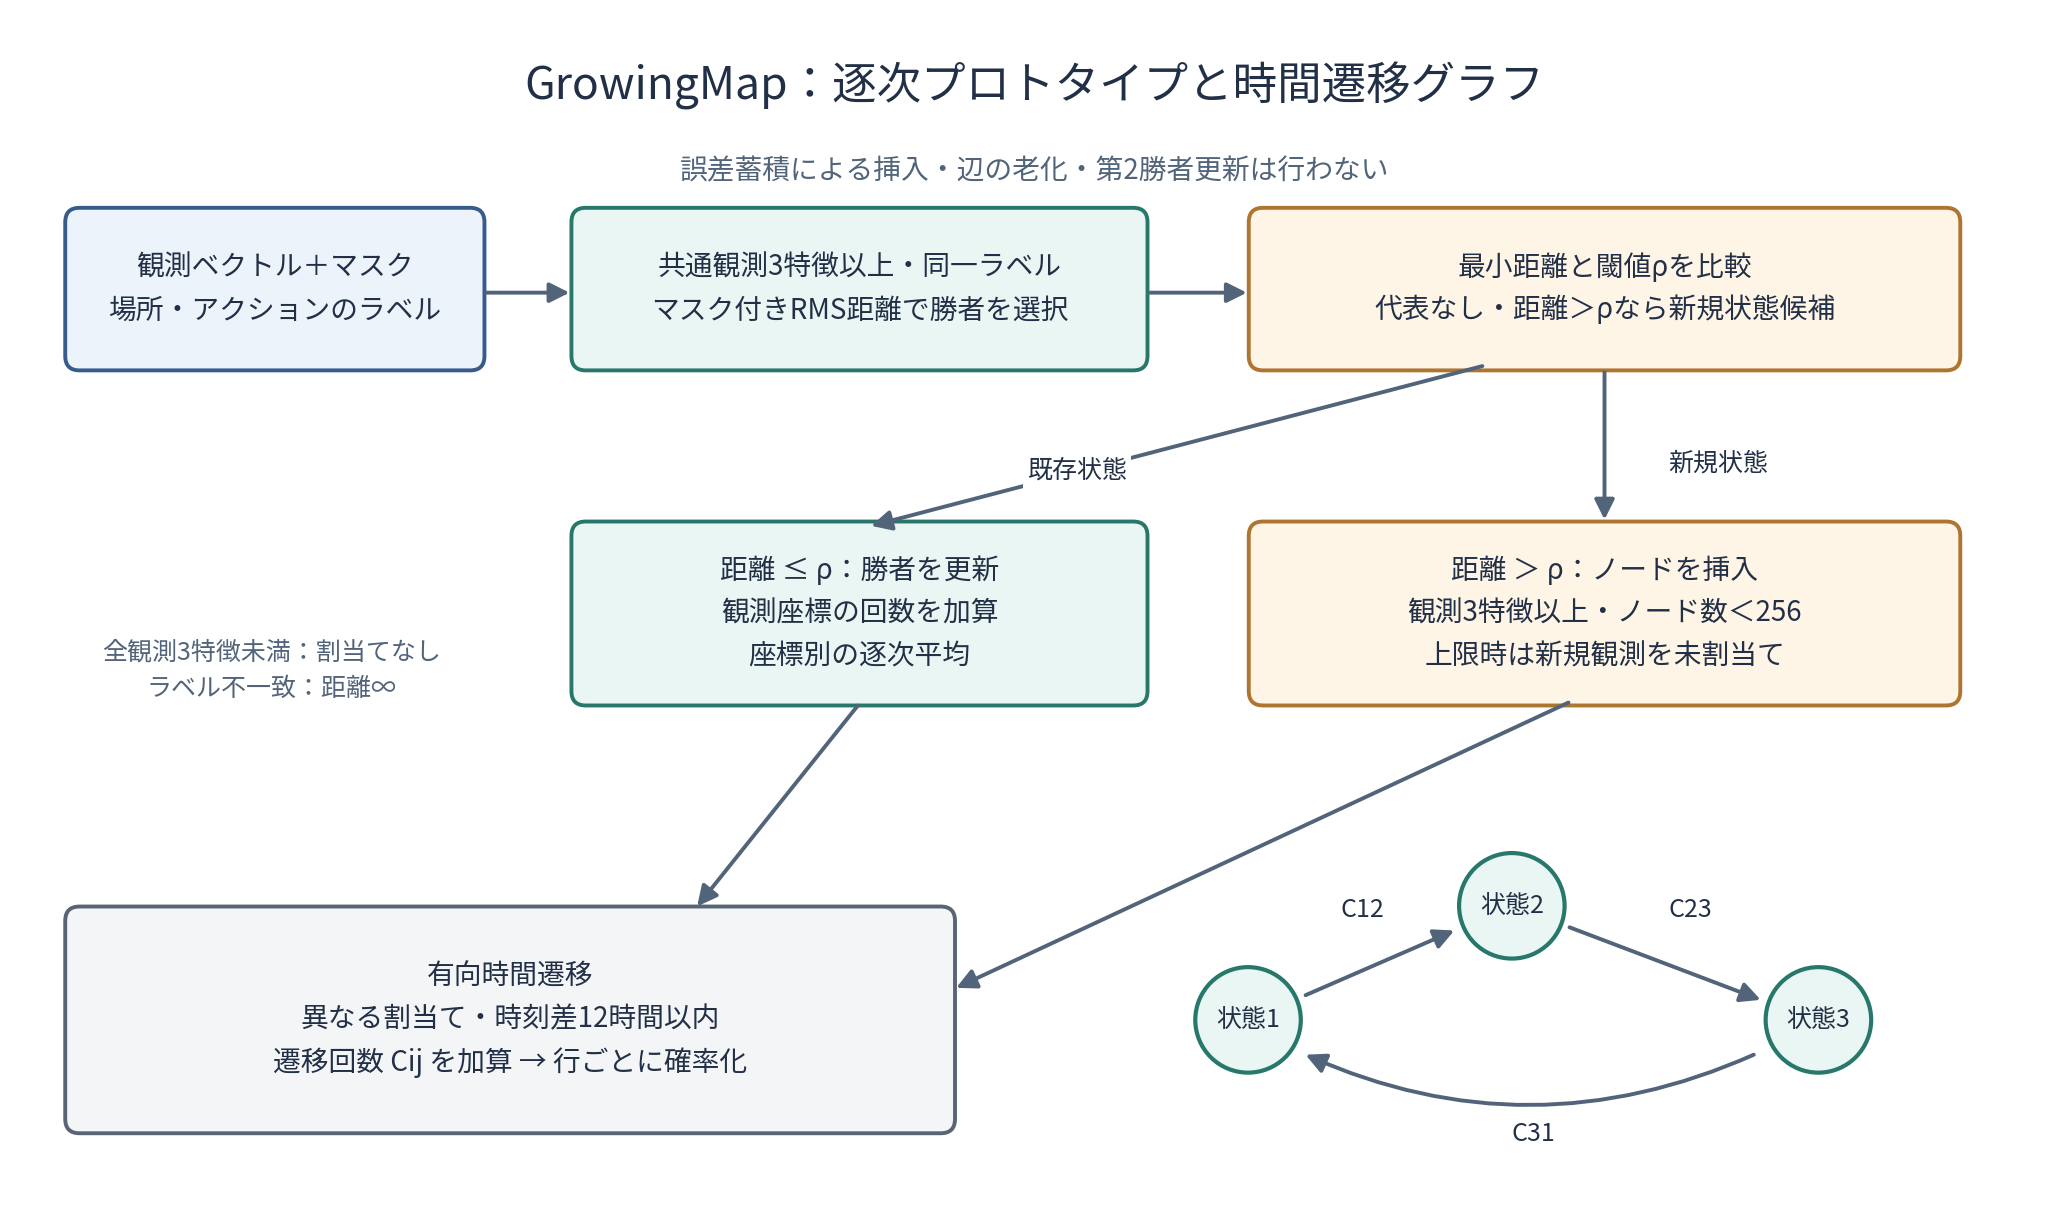
\includegraphics[width=\linewidth,height=180mm,keepaspectratio]{figures/fig_growingmap.png}
  \caption{従来構成のGrowingMapの処理フロー。観測マスクとラベルが一致する代表から勝者を選び、既存ノードの座標別逐次平均更新または閾値による新規ノード生成を行う。図中の矢印は処理順序を示す。状態ノード間の辺には条件を満たす状態変更回数を保存し、構成比は回数から導出する。新方式のDiscoveryMapを示す図ではない。}
  \label{fig:legacy-growingmap}
\end{figure}

\section{時系列推定と個人適応の基盤}

生活状態推定には、入力の時間依存性を表現する学習器と、欠測を除外した教師損失が必要である。本人の履歴による条件付け、逐次重み更新、部分プーリングは、従来構成または拡張比較に属する。表現の記憶、勾配の伝播、推定時に利用できる回答の範囲を別の条件として定義することで、各機構の効果を検証できる。

\subsection{LSTMのゲートとセル状態}

LSTMは、セル状態を通じて過去の情報を保持する再帰型モデルである \autocite{hochreiter1997lstm}。本研究が用いる忘却ゲートを含む形は、初期のLSTMに対する後の発展を含む \autocite{gers2000forget}。入力\(\boldsymbol{x}_t\)、前時点の隠れ状態\(\boldsymbol{h}_{t-1}\)、セル状態\(\boldsymbol{c}_{t-1}\)に対し、各ゲートと候補は

\[
\begin{aligned}
\boldsymbol{i}_t&=\sigma(W_i\boldsymbol{x}_t+U_i\boldsymbol{h}_{t-1}+\boldsymbol{b}_i),\\
\boldsymbol{f}_t&=\sigma(W_f\boldsymbol{x}_t+U_f\boldsymbol{h}_{t-1}+\boldsymbol{b}_f),\\
\boldsymbol{o}_t&=\sigma(W_o\boldsymbol{x}_t+U_o\boldsymbol{h}_{t-1}+\boldsymbol{b}_o),\\
\widetilde{\boldsymbol{c}}_t&=\tanh(W_g\boldsymbol{x}_t+U_g\boldsymbol{h}_{t-1}+\boldsymbol{b}_g),\\
\boldsymbol{c}_t&=\boldsymbol{f}_t\odot\boldsymbol{c}_{t-1}
+\boldsymbol{i}_t\odot\widetilde{\boldsymbol{c}}_t,\\
\boldsymbol{h}_t&=\boldsymbol{o}_t\odot\tanh(\boldsymbol{c}_t)
\end{aligned}
\]

となる。\(\sigma\)はシグモイド関数、\(\odot\)は要素積である。\(W\)は入力から、\(U\)は前の隠れ状態からの重みを表す。PyTorchでは入力側と再帰側に別々のバイアスを持つため、式の\(\boldsymbol{b}\)は両者の和と解釈できる。

入力ゲートは新しい候補を取り込む量、忘却ゲートは過去セルを残す量、出力ゲートはセルを隠れ状態へ読み出す量を制御する。各ゲートは学習されるため、時間が経過すれば必ず一定割合で忘れるという固定規則ではない。セルの加法的な更新経路は過去の情報を保持する助けとなるが、長い依存が常に正確に学習されることを保証しない。系列長、教師信号、最適化、入力の観測密度を併せて評価する必要がある。

\subsection{状態保持とTruncated BPTT}

系列を複数のチャンクへ分けると、順伝播の状態を引き継ぐか、逆伝播をどこまで行うかという二つの選択が生じる。Truncated Backpropagation Through Time（TBPTT）は、時間方向の勾配を有限の範囲へ制限する方法である \autocite{williams1990tbptt}。チャンク\(j\)の最終状態を\(\boldsymbol{s}_{j}^{\mathrm{end}}=(\boldsymbol{h},\boldsymbol{c})\)とし、次の初期状態を

\[
\boldsymbol{s}_{j+1}^{\mathrm{start}}
=\operatorname{sg}(\boldsymbol{s}_{j}^{\mathrm{end}}),\qquad
\frac{\partial\operatorname{sg}(\boldsymbol{s})}{\partial\boldsymbol{s}}=0
\]

とすると、値は保存されるが前チャンクへの勾配は切断される。チャンク損失\(\mathcal{L}_j\)に対する\(\nabla_\theta\mathcal{L}_j\)は、そのチャンク内の計算グラフから計算する。状態をゼロに戻す操作は、値の記憶も失うため、勾配だけを切る操作とは異なる。

従来の状態保持型拡張の比較計画では、Microは同じ作業区間、Mesoは同じ日内という条件下でのみ状態を保持する。参加者の切替え、意味単位の境界、長い欠測では初期化する。Macroは過去28日の明示的な入力窓が長期情報を担うため、チャンク間で状態を持ち越さない。区間・日・週の境界へチャンクを整列させ、境界を越えて異なる意味の状態を連結しない。この状態保持を\texttt{life-discovery-v1}の実装済み設計とは扱わない。

現行の運用コードは、学習例をシャッフルしたミニバッチによるバッチ学習であり、LSTMの初期状態を学習例間で引き継がない。TBPTTおよび逐次状態保持は未実装の比較計画として位置付ける。推論の反復実行、モデルの再学習、LSTM内部状態の持越しは、それぞれ別の処理である。

\subsection{自己報告による個人適応}

個人適応には、過去回答から作る特徴で予測を条件付ける方法と、回答を教師としてモデルの重みを更新する方法がある。従来構成の履歴条件付けは、全履歴、同じ時刻帯、同じ曜日、同じ活動における五尺度の平均と有効性マスクを利用する。特徴\(\boldsymbol{a}_{p,t}\)を変換して表現へ加える操作\(\boldsymbol{r}'_{p,t}=\boldsymbol{r}_{p,t}+g_\theta(\boldsymbol{a}_{p,t})\)は、推論時のパラメータ更新を伴わない。新方式ではこの回答履歴変換を持たず、観測を入力、本人確認と尺度回答を教師として分離する。

重みを更新する個人適応の比較はprequential評価として扱う。時点\(t\)で予測し、その後に受信された回答を将来の更新へ利用する。利用集合を\(\mathcal{A}_p(t)=\{a:t_a^{\mathrm{target}}<t,\ t_a^{\mathrm{received}}<t\}\)とし、同じ回答を繰り返して新規回答として扱わない。遅延回答は対象時点の後でしか利用できず、その回答で更新したモデルを対象時点へ遡って評価すると情報漏洩になる。新方式のライブ推論中にこの重み更新を行う実装はない。

従来構成の比較では、参加者内で学習したモデルを起点とする更新と、条件付けの有無を分ける。全参加者共通の事前学習済みグローバルモデルから個人へ転移する運用機構は存在しない。回答が少ない場合には、重み更新の自由度が高いほど過適合や変動が生じ得るため、凍結条件と更新範囲を制限した条件を同じ予測順序で比較する。

\subsection{自己教師あり学習による表現形成}

自己教師あり学習は、観測自体から学習対象を作り、本人回答がない区間も表現学習へ利用する方法である。BERTはマスクされたトークンの予測を通じて言語表現を学習し \autocite{devlin2019bert}、Masked Autoencodersは画像の一部を隠して再構成する学習を扱う \autocite{he2022mae}。SimCLRは変換した入力間の対比を用いる別の系列の方法である \autocite{chen2020simclr}。これらは自己教師信号の設計例であり、本研究の損失がトークン予測や画像再構成と同一であることを意味しない。

従来構成のSSL実験経路では、観測特徴のランダムマスク再構成と、5〜30分先の特徴予測を組み合わせる。再構成では未観測値を正解にせず、隠した観測座標だけへ誤差を与える。文章埋め込みは意味のまとまりとしてブロック全体を隠し、残った座標から隠れた座標を容易に復元することを抑える。将来予測では入力を時点\(t\)以前へ限定し、教師となる将来特徴を学習区間内から作る。

従来構成の比較計画には、SSL事前学習の後、活動分類と五尺度の教師損失でファインチューニングする二段階学習を含める。事前学習に使うのは対象の参加者データ系列であり、別に存在する全参加者共通モデルを前提にしない。検証・評価期間の未ラベル観測を事前学習へ入れることも、将来情報の利用として排除する。

提案方式では、最新ビンの観測済み特徴を確率0.2で隠す再構成、PlaceとBehaviorからの次1時間の観測予測、本人確認IDの関係損失、現在・日次尺度のHuber損失を同時に最適化する。各埋め込みには縮退を抑える分散項を加える。二段階の事前学習を必須とせず、24クラスの交差エントロピーを含めない。マスクや教師の有効性、係数を含む正確な損失構成は第\ref{chap:model}章\ref{sec:joint-learning}節で示す。

\subsection{階層モデルと部分プーリング}

参加者ごとに完全に別のモデルを学習する方法では、回答数の少ない参加者の推定が不安定になりやすい。一方、全参加者へ同一の平均を当てはめると、尺度の使い方などの個人差を表せない。部分プーリングは、共有構造と個別の効果を組み合わせ、個別効果を共通の中心へ収縮させる考え方である \autocite{gelman2007multilevel}。

五尺度の共有出力を\(f_\theta(\boldsymbol{x}_{p,t})\)、参加者別バイアスを\(\boldsymbol{b}_p\in\mathbb{R}^5\)とすると、

\[
\widehat{\boldsymbol{y}}_{p,t}
=f_\theta(\boldsymbol{x}_{p,t})+\boldsymbol{b}_p,\qquad
\mathcal{J}=\sum_{p,t}\mathcal{L}_{p,t}
+\lambda\sum_p\|\boldsymbol{b}_p\|_2^2
\]

と定式化できる。二乗罰則は、\(\boldsymbol{b}_p\sim\mathcal{N}(\boldsymbol{0},\tau^2I)\)のガウス事前分布に対応するMAP推定の解釈を持つ。従来構成の部分プーリング実験経路では、共有出力と個人バイアスに対する二乗誤差と収縮罰則を用いる。従来基本モデルと提案方式の尺度出力が用いるHuber損失とは区別し、完全な階層ベイズ推論や不確実性の事後分布の計算は行わない。参加者間の部分プーリングは\texttt{life-discovery-v1}には実装されていない。

回答数が少ない個人のバイアスをゼロへ強く制約し、十分な回答がある場合に共有出力からの差を学習する。受信済み回答だけでバイアスを更新する条件、全層を更新する条件、凍結する条件を比較すれば、低い自由度の個人差モデルが逐次評価で安定するかを検討できる。共有エンコーダを実験内で共同学習する設計と、事前に完成したグローバルモデルの存在は区別する。

\section{本人の解釈を保持する情報モデル}

自己報告は、観測の正解を一度だけ付けて完了する操作とは限らない。本人が時間を置いて状態を捉え直したり、推定の誤りを訂正したりするため、記録の対象時点と追加された時点を分けて保持する必要がある。観測、機械推定、提示の根拠、本人の回答を混在させると、どの情報に依存した推定であるかを再現できなくなる。以下では、従来構成のナラティブ記録とPMTTを背景として整理する。情報の役割を分ける考え方は提案方式でも保持するが、PMTTを新しいパターン発見器の一部とはしない。

\subsection{お天気分とナラティブポートフォリオ}

お天気分は、本システムでは本人が主観的な気分を短い選択で表す入力として扱う。入力契約上の値はhappy、normal、sad、angryである。この分類は五尺度の数値回答と異なるため、「happyなら気分5」などの換算をせず、独立した本人の表現として保存する。表現が簡潔であることは、気分のすべての側面が区別されることを意味しない。

ナラティブポートフォリオは、本論文では本人の状態記述、回答、修正を時間順に蓄積し、振り返り可能にする考え方として扱う。特定の外部尺度や標準化された診断法との同等性は前提としない。自由な状態の表現、従来分類の活動カテゴリ、五尺度、提案方式の拠点・行動確認には、異なる情報の粒度がある。提案方式では本人確認と尺度回答を教師に用い、活動回答は事後注釈へ位置付ける。本人の自由な表現をいずれかの教師へ強制的に還元せず保持する。

この設計により、数値は似ていても本人が異なる意味を与えた記録を、同一の経験としてまとめずに済む。また、入力の訂正が増えた理由として誤入力、推敲、変換などを回答できる仕組みは、操作の変化を直ちに疲労と解釈することを避ける助けとなる。本人の解釈を観測値の代わりに用いるのではなく、観測の意味を確認する別の記録として対応付けることが重要である。

\subsection{従来構成のPMTTによる情報の分離}

従来構成のPMTTを記録の由来をたどるグラフ\(G=(V,E_G)\)とする。\(V\)は記録のノード集合、\(E_G\)は関係を表す有向辺集合である。情報の役割を\(\mathcal{O}\)（観測）、\(\mathcal{I}\)（推定）、\(\mathcal{E}\)（根拠）、\(\mathcal{R}\)（本人の回答・修正）で表し、第\ref{chap:model}章の役割表記へ統一する。概念上の対応は

\[
\mathcal{O}\xrightarrow{\mathrm{used\ by}}\mathcal{I},\qquad
\mathcal{E}\xrightarrow{\mathrm{supports}}\mathcal{I}\ \text{または提案},\qquad
\mathcal{R}\xrightarrow{\mathrm{targets}}\mathcal{I}\ \text{または対象区間}
\]

である。役割の分離は、保存上のすべての記録が四種類の専用ノード型を持つことを要求しない。従来APIでは観測、推定、narrative、correctionなどをObservation型で包み、source属性で区別する。これらを毎正時のStateEpisode、Day、月曜起点の固定週Patternへ関連付ける。運動提案はExerciseProposalとして根拠と対応付けられる。この保存の背景は、提案方式で新しい状態に基づく運動提案が実装・検証済みであることを意味しない。

修正記録\(r\in\mathcal R\)は、対象区間、追加時刻、参照ID、修正内容を持つ。元の観測\(o\in\mathcal O\)や推定\(i\in\mathcal I\)を削除して新しい値へ置き換えるのではなく、修正を追加して当時の推定を残す。学習データを作る際に利用可能な修正を選ぶ処理と、履歴の表示は分ける。このため、現在の本人回答と、過去の時点で利用できた本人回答の双方を再構成できる。

PMTTは時間枠に沿う由来の構造であり、未知の行動パターンを自動発見する学習器ではない。GrowingMapの状態ノードとPMTTの時間枠ノードを同一視せず、状態割当てを持つ観測記録を介して対応させる。由来グラフを保持しても、モデルの判断全体が因果的に説明されたことにはならず、どの入力と基準を用いたかという検証可能性を支える。

\section{既存研究の課題と本研究の位置付け}

先行研究から、本研究に関わる課題は三つに整理できる。第一に、異種ライフログの値を時間軸上で統合するだけでは、その値が当時利用できたかを保証できない。イベント時刻と受信時刻の双方を用いた因果カットオフ、任意同意と欠測の区別、ラベル対象区間の定義が必要である。第二に、操作、日内文脈、複数日の履歴を一つの表現へ単純に平均すると、順序と時間尺度の差が失われる。第三に、本人の回答を取得しても、それが推定の上書きとして保存されると、過去の予測と修正の関係を評価できない。

本研究は、研究用キーボードから得る操作特徴とローカル文章特徴を中心に、任意同意の生活情報を加える。文章表現にはSentence-BERTに基づく文埋め込みを利用し \autocite{reimers2019sentencebert}、小型言語モデルの基盤としてMiniLMを参照する \autocite{wang2020minilm}。主条件は研究サーバ上のローカルSentenceTransformerの\path{paraphrase-multilingual-MiniLM-L12-v2}であり、384次元の埋め込みを固定ランダム射影で32次元へ変換する。従来構成と新方式に共通する入力基盤であり、比較時は同一のモデルrevision・内容ハッシュ・射影を固定する。未指定時の文字n-gram経路は別条件である。原文を外部AIサービスへ送らない設計とするが、埋め込み化は個人情報の完全な匿名化を保証する操作ではない。

提案方式は、共有三階層LSTM、Place・Behaviorの独立射影、訓練側で構築するDiscoveryMap、現在・日次5尺度の回帰を主構成とする。自己教師ありの再構成・次1時間予測と本人確認・尺度教師を同時に用い、推論時には重みとマップを凍結する。\texttt{task}はBehaviorの保存・通信上の互換名であり、独立した第三の推定器ではない。

従来の固定24活動分類、独立ContextLSTM、生観測GrowingMap、PMTT、回答履歴条件付け、二段階SSLおよび部分プーリングは、背景・比較条件として保持する。本人平均・前回値などの基準予測との比較も、同じ時点と有効教師にそろえて行う。新方式は\texttt{research\_architecture=discovery}で明示選択し、サーバーの既定は\texttt{legacy}である。主構成の更新と既存運用の切替を区別する。

これらの統合が生活状態推定に有効であるかは、実験前には確定できない。少人数・短期間の予備研究では、取得の継続性と回答負担を主に検討し、推定性能は時間順分割と同一対象での比較により探索的に評価する。理論上の表現力、コードとして実装された処理、評価予定の処理を区別することが、本研究の検証可能な位置付けとなる。

\chapter{生活情報の観測と学習データ構築}
\label{chap:observations}

生活状態モデルが受け取るのは、状態そのものではなく、研究用キーボードや生活情報の取得系を通じた不完全な観測である。操作のない時間、収集が停止した時間、本人が提供を選ばなかった情報を区別しなければ、生活の変化と計測条件の変化が混同される。提案構成では、観測入力、本人確認、5尺度の教師、事後の活動注釈を分離して保存・処理する。

\section{観測過程と利用可能時刻}

参加者\(p\)の潜在的な生活状態を\(s_p(t)\)とすると、情報源\(a\)の観測は\(o^{(a)}_{p,i}=g_a(s_p(t_i),\eta_{p,i},c_{p,i})\)と表せる。\(\eta\)は計測誤差、\(c\)は端末利用・取得許可などの条件である。情報源ごとに観測写像が異なるため、入力回数の変化を疲労の変化と直接同一視しない。

論理的なイベント記録は、参加者、情報源、識別子、発生時刻、受信時刻、値、メタデータの組として表す。

\[
e_i=(p_i,a_i,\mathrm{id}_i,t_i^{\rm occ},t_i^{\rm recv},v_i,\kappa_i).
\]

\(p_i\)は参加者、\(a_i\)は情報源、\(\mathrm{id}_i\)は識別子、\(t_i^{\rm occ}\)は発生時刻、\(t_i^{\rm recv}\)は収集サーバの受信時刻、\(v_i\)は観測値、\(\kappa_i\)は同意や仕様を識別するメタデータである。推定時刻\(T\)で利用する観測には\(t_i^{\rm occ}\le T\)かつ\(t_i^{\rm recv}\le T\)を要求する。収集サーバと研究サーバを分ける場合も、元の受信時刻を保持して複製し、研究サーバの処理時刻に置き換えない。後から到着した記録を、過去の予測時点で既知だったものとして扱わない。

この因果的な利用条件を、時間窓\(B\)と参加者\(p\)に対する集合として明示する。\(\chi_i^{\rm obs}\)を、記録\(e_i\)が同意条件を満たす観測入力であり、質問回答やモデル推定ではない場合に1となる指示変数とすれば、

\[
\mathcal O_p(B;T)=
\left\{e_i:\ p_i=p,\ t_i^{\rm occ}\in B,\
t_i^{\rm occ}\le T,\ t_i^{\rm recv}\le T,\ \chi_i^{\rm obs}=1\right\}.
\]

\(\mathcal O_p(B;T)\)がその窓の特徴生成に利用できる記録の集合である。\(\mathbf1[\cdot]\)を条件が成立すると1、成立しなければ0となる指示関数とし、以後の存在指示にも用いる。同じ発生時刻の記録であっても受信時刻が異なれば、異なる推定時点で利用可能になる。したがって、窓の集約値は\(B\)だけでなく入力カットオフ\(T\)にも依存する。

Macを収集サーバ、Ubuntuを研究サーバとする構成では、このカットオフはMacで利用可能だった情報集合を表す。複製後の記録から特徴を再構成しても、Ubuntuへの転送遅延まで含めた当時の利用可能性を証明するものではない。収集サーバの受信時刻に基づく評価と、研究サーバでの実際の到着・処理・端末表示までを含む評価を分ける。

\subsection{同意と欠測}

研究用キーボードの入力・削除・確定操作を主な観測とし、歩数、予定、開閉センサは任意同意の補助情報とする。情報源の利用許可\(c_{p,a}\)と、許可下での観測存在\(r_{p,a}\)を分け、観測可能性を\(m_{p,a}=c_{p,a}r_{p,a}\)で表す。presenceだけでは未同意と通信障害の原因を判別できないため、設定・収集状態も保存する。

歩数の提供と運動提案の有効化は別の同意・設定である。入力原文の取得経路と、モデルへ数値特徴を渡す経路も区別する。ローカル文章処理は外部サービスへの原文送信を避けるが、特徴ベクトルの匿名性や無制限利用を保証するものではない。

\subsection{時間単位と回答対象}

時刻にはタイムゾーンを要求し、日付境界は日本標準時の午前0時、週境界は月曜日の午前0時とする。質問の対象時刻\(t^{\rm target}\)、端末での回答完了\(t^{\rm ans}\)、受信\(t^{\rm recv}\)を分離する。回答が端末に存在しても、受信前のサーバ推定には使わない。

提案構成のMicro入力は5分ビン、区間は正時で分けた最大1時間である。Mesoは日内の区間列、Macroは当週の日表現と先行28日の日別観測を扱う。従来方式にあった活動回答・訂正による区間分割は、新しい観測入力には適用しない。本人確認時刻は教師例の追加に用いるが、その回答内容を観測系列へ入れない。

\section{キーボード由来の特徴}
\label{sec:keyboard-features}

研究用キーボードは他のキーボードや、入力しない活動を網羅しない。操作統計に加え、セッション、最終観測からの経過時間、heartbeat、収集有効状態を保持する。質問回答用操作は\texttt{purpose=assessment}によって通常の入力特徴から除外する。

heartbeatは、親アプリのcontext更新時と、Full Accessがあるキーボードの出題判定時に送信を試みる。親アプリは\texttt{source=parent\_app}と質問設定を報告し、キーボードの収集状態を推測しないため\texttt{logging\_enabled}を省略する。キーボードは\texttt{source=keyboard}として、プライベートモードを反映した収集設定と質問設定を報告する。質問機能がOFFでも動作時には報告を試みるが、Full Accessがないキーボードからは送らない。

このheartbeat送信は1回の通信であり、永続キュー・再送・応答による到達確認を行わない。セッションや回答の永続送信とは保存契約が異なる。heartbeatがない時間を、収集停止や無操作の確定として扱わず、アプリを閉じた後も定期報告が継続するとは仮定しない。

\subsection{操作統計と通常との差}

区間\(B=(u,v]\)に含まれ、推定時刻\(T\)までに受信された打鍵時刻を\(\tau_1<\cdots<\tau_n\)とする。打鍵数、削除数、確定文字数に\(\log(1+x)\)を適用して計数値の尺度を圧縮し、間隔\(\delta_j=\tau_j-\tau_{j-1}\)から次の統計を計算する。

\[
\bar\delta_B=\frac1{n-1}\sum_{j=2}^{n}\delta_j,\qquad
\delta_B^{\max}=\max_{2\le j\le n}\delta_j,\qquad
N_B^{\rm pause}=\sum_{j=2}^{n}\mathbf1[\delta_j>2\,\text{秒}].
\]

平均・最大間隔は分単位、休止数は対数変換した値とする。\(n<2\)では間隔を未観測とし、架空のゼロ秒を作らない。セッション、打鍵、または5分以内の収集中heartbeatによって観測範囲が確認できる場合に限り、打鍵ゼロを観測された無操作として表す。

訂正率の通常との差を検出する\texttt{typing\_change}は、LSTMとは別に固定10分窓を使う。\texttt{kana}・\texttt{text\_insert}の物理的挿入と本人の削除を対象とし、一般の\texttt{key}イベントをすべて挿入とはみなさない。質問回答操作を除外し、2秒以内の連続削除を一つの訂正バーストへまとめる。

端末・入力モードごとに日\(d\)の挿入数\(I_d\)、訂正バースト数\(B_d\)をプールし、\(R_d=B_d/I_d\)を得る。\(I_d\ge50\)を有効日とし、過去3〜4有効日は暫定、5有効日以上は正式とする。当日を\(d_0\)、有効日の訂正率の99パーセンタイルを返す演算を\(Q_{0.99}\)とすると、検出閾値\(\theta\)は

\[
\theta=\max\{Q_{0.99}(\{R_d\}_{d<d_0,\ I_d\ge50}),0.02\}
\]

である。当日と直前有効日の率がともに閾値を超えることを要求する。これは誤入力の確定でも、別の行動分類器でもない。

\subsection{ローカル文章表現}
\label{sec:sentence-encoder}

文章特徴には各窓の確定イベントから構成した文字列だけを使う。候補置換が観測済み接尾部に一致する場合は、その部分を新しい確定内容に置き換える。窓より前の文章を含む文書全体を復元する処理ではない。入力前後のcontext文字列は保存・エクスポートされても、重複や他者情報の混入を避けるためモデル特徴に含めない。入力文字列は末尾4096文字以内に制限し、採用モデルのtokenizerが最大128トークンへ切り詰める。4096文字すべての意味が保持されるとは限らない。

LocalEncoderは研究サーバ上のローカルSentenceTransformerを凍結して使用する。iOSは確定イベントを収集サーバへ送り、文章の埋め込み生成、生活状態モデルの学習・推論、候補マップの構築はサーバ側で行う。原文を外部AIサービスへ送らないことと、iPhoneから研究用のサーバへ収集記録を送ることは異なる通信条件である。採用するモデルとrevisionは以下である。

\begin{itemize}
\item
  モデル：\texttt{sentence-transformers/paraphrase-multilingual-MiniLM-L12-v2}
\item
  revision：\texttt{e8f8c211226b894fcb81acc59f3b34ba3efd5f42}
\end{itemize}

文単位の表現学習の基礎にはSentence-BERTがあり\autocite{reimers2019sentencebert}、採用モデルの基盤にはMiniLMがある\autocite{wang2020minilm}。使用する384次元の正規化済み埋め込み\(E(w)\)を、固定ランダム射影\(R\in\mathbb R^{384\times32}\)によって32次元へ変換する。

\[
e(w)=\frac{E(w)R}{\max(\lVert E(w)R\rVert_2,10^{-8})},\qquad
R_{jk}\sim\mathcal N(0,1/32).
\]

ここで\(w\)は窓内で構成した入力文字列、\(E(w)\in\mathbb R^{1\times384}\)は行ベクトルとして表した文埋め込み、\(e(w)\in\mathbb R^{1\times32}\)は射影後の文章特徴である。\(R_{jk}\)の\(j=1,\ldots,384\)は入力座標、\(k=1,\ldots,32\)は射影先座標を表す。\(\mathcal N(0,1/32)\)は平均0・分散\(1/32\)の正規分布、\(\lVert\cdot\rVert_2\)はユークリッドノルムである。\(R\)と文エンコーダは時系列モデルの学習時にも更新しない。以下で特徴を列ベクトルとして連結するときには\(e(w)\)を転置して用いる。

射影seedは17で固定し、LocalEncoderのメタデータには入力・出力次元、射影seed、モデルファイルの内容ハッシュと、配置時に保存した出典情報を保持する。384次元は採用モデルの構成であり、実装は読み込んだモデルの埋め込み次元を取得して射影行列を作る。\texttt{local\_files\_only=True}、\texttt{trust\_remote\_code=False}で読み込み、推定時に原文を外部APIへ送信しない。新方式の学習記録にはローカルモデルのパスと内容に基づく\texttt{text\_identity}を保存し、推論時に同じ識別情報であることを確認する。

従来の通常・文脈・実験CLIとサーバー設定例では、同じローカルモデルを指定する。従来CLIの既定パスは\path{data/text-models/paraphrase-multilingual-MiniLM-L12-v2}であり、文字n-gramとの比較には\texttt{-\/-character-ngram}を明示する。一方、新方式の\path{research.discovery_cli}は\texttt{-\/-text-model}の既定値が未指定であるため、SentenceTransformerを主条件とする学習では同オプションにローカルモデルのパスを明示する。サーバーでも\texttt{text\_model}へ同じパスを設定する。指定したモデルが欠落・破損している場合はエラーとし、文字n-gramへ自動で切り替えない。

モデルを指定しないAPI・新方式CLI・未設定サーバーでは、文字1・2・3-gramの符号付きハッシュによる32次元表現を使う。この経路を事前学習言語モデルの意味理解と同一視しない。従来のSSL用系列でも、回答を除去したTimelineへ同じ文章モデルを渡す。文章エンコーダの変更後は時系列モデルを再学習し、旧重みをそのまま利用しない。導入したモデルと実データにおける精度改善は別の検証事項である。空文字列は零ベクトルで、文字数と観測範囲を併用する。

\section{任意同意の生活情報}

歩数の増加は身体活動の手がかりだが、その目的や集中度を確定しない。予定の存在と実行、開閉状態と本人の在室も一致するとは限らない。値と取得時刻・鮮度を保持し、情報源が直接示す範囲を超えて教師を生成しない。

\subsection{歩数・健康指標・予定}

HealthKitと予定は親アプリで取得し、App Groupのcontextに保存してキーボードのセッション送信へ添付する。歩数・歩行距離・階段・活動エネルギーは日本時間の当日午前0時から取得時点までの合計、歩行速度・歩幅・左右非対称性は直近1時間の平均である。HealthKitのバックグラウンド更新は毎時の頻度で登録するが、実行時刻はiOSに依存し、正確な1時間間隔の観測を保証しない。

LSTM特徴の\texttt{steps}は、新鮮な日累積値\(P_i\)に対する\(\log(1+P_i)\)である。一方、従来の状態内歩数の集計には同一参加者・端末・日の差分\(\Delta P_i=\max(0,P_i-P_{i-1})\)を使い、前観測なし、累積値減少、観測間隔900秒超、日跨ぎを除外する。従来の提案用歩数保存では15分以内の鮮度も要求する。これらは長い欠落中の歩数を後側の状態へ誤帰属させないための条件である。区間増分と累積値、および学習特徴と提案用の鮮度基準を同じ量・条件として説明しない。新方式の行動IDに基づく歩数基準は未検証であり、その提案経路は停止する。

歩行距離、階段、活動エネルギー、歩行速度、歩幅、左右非対称性も取得可能な範囲で扱う。モデル特徴では項目別更新時刻が2時間以内の有限値を使う。旧形式で項目別時刻がない場合は鮮度を確認できないため、観測値として利用しない。

項目別の取得時刻は\texttt{measurement\_updated\_at}に保持し、別項目の更新でcontext全体の\texttt{updated\_at}が新しくなっても、古い値の取得時刻は更新しない。電池残量と電池状態は同じ取得時刻を付ける。親アプリのheartbeat自体にはこれらの計測値を載せないため、heartbeatが届いたことだけで健康・予定の観測が新鮮になったとは扱わない。

予定は推定時刻が予定区間に含まれるかを示す\texttt{calendar\_busy}と、予定件数の対数値\texttt{calendar\_count}へ変換する。開始・終了を\(a_j,b_j\)とすれば、\(c_{\rm busy}(T)=\mathbf1[\exists j:a_j\le T<b_j]\)である。予定タイトルの埋め込みは98次元へ追加しない。予定ゼロも取得可否と鮮度が確認できる場合に限り観測とする。

\subsection{開閉センサと拠点}

玄関・寝室に対応するセンサ状態と経過時間を扱う。推定時刻までに利用できる最後の観測を\(j^*\)とすると、\(q(T)=q_{j^*}\)は状態の復元値である。長時間の状態保持には周期的なBLE観測が必要となる。特徴生成は変化イベントと周期観測の両方を受け入れ、最終観測から120秒以内の場合に状態を有効とする。\texttt{close}を0、\texttt{open}と\texttt{timeOutNotClose}を1とし、未知・鮮度不足ではpresenceを0にする。最終観測からの経過時間は別座標に保持する。センサ名は計測箇所の識別であり、本人の居場所の教師ラベルではない。

PlaceとBehaviorには第\ref{chap:model}章の共有エンコーダを使う。GPS、Wi-Fi識別子、RSSI、旧場所訪問イベントは観測入力に含めない。従来の独立ContextLSTMは比較条件であり、提案構成の一部として同時学習しない。

\section{本人回答と教師・注釈の役割}

Place・Behaviorの同一性確認、現在・日次5尺度、固定24活動の回答を区別する。Place・Behaviorの確認は各軸の関係学習に使い、尺度は回帰教師、24活動はモデル・マップを固定した後の説明注釈と旧分類器の教師に使う。本人確認なしのクラスタIDを正解として自己循環させない。

\subsection{場所・行動の確認と命名}
\label{sec:context-confirmations}

質問は\texttt{placeCheck}と\texttt{taskCheck}を維持する。新方式の\texttt{task}はBehaviorの互換名であり、24活動とは別の固定分類表を持たない。回答は質問発行時までの5分区間のラベルとして保存する。通信が遅れた回答を、回答受信時の新しい場所や作業の正解にしない。

両軸の確認質問は合計で1日1件まで発行し、直前に発行した確認質問の軸を基準に交互に選ぶ。選択には、当日終了したセッションが発行時刻から3時間以内にあり、発生・受信ともその時刻以前であることを要求する。確認質問の有効期限は発行から30分で、回答対象は発行前5分のままである。この3時間は質問選択だけの条件である。モデルの学習例・推論は、対象時刻から遡って1時間以内に終了し、その時刻までに受信されたセッションを要求する。質問に回答できても、その対象時刻が学習の鮮度条件を満たすとは限らない。

Web画面では軸ごとの区間訂正、分割、命名、統合を追記する。名前だけの変更は同一性の教師を増やさない。「わからない」と「移動中」は確定IDの学習対に含めない。場所を変えずに行動だけを訂正すること、およびその逆を可能にする。

\subsection{5尺度と固定活動注釈}
\label{sec:scales-and-activity-labels}

質問画面の尺度順序を気分・疲労・ストレス・集中度・眠気とし、選択肢は\(y_k\in\{1,2,3,4,5\}\)である。入力検証は範囲内の有限な数値を受け入れるため、画面の5段階選択とは区別する。全尺度を悪化方向へ一括変換しない。現在と日次のscopeを分け、有効性は\(m_k^y=\mathbf1[y_k\text{が有限で }1\le y_k\le5]\)とする。新方式は欠測を非有限値で保持し、有効座標だけを損失に用いる。従来方式の尺度損失で使用する補完値3も計算用であり、本人が3と答えたことを意味しない。自由記述から数値として検証できない内容や、全尺度が無効な回答を回帰教師にしない。

固定活動注釈は、デスクワーク、会議・打合せ、勉強・研究、料理、掃除、洗濯、買い物、食事、入浴、トイレ、身支度、くつろぎ、仮眠、就寝準備、テレビ・動画、ゲーム、読書、スマホ・SNS、散歩、通勤・通学、用事、家族と、友人と、通話の24種類である。この既存回答は保持するが、提案モデルの出力次元や損失、入力区間の分割に用いない。行動と社会的文脈が混在する分類体系であることも、事後の意味対応を解釈する際に考慮する。

現在・日次の尺度回答は\texttt{currentState}・\texttt{nightReflection}として別に保存し、回答ラベルは\texttt{current\_state}・\texttt{daily\_reflection}、有効な項目の値はJSONで保持する。親アプリの活動カタログ回答は、表示名とは別に\texttt{desk\_work}等の安定値を\texttt{answer.label}へ保存する。自由入力に含まれる内容を、そのまま新しい固定活動ラベルや尺度教師へ変換しない。

\subsection{対象時刻と受信時刻}

現在状態の入力カットオフは質問提示時刻を優先し、記録がなければ検出時刻を使う。回答完了までに生じた観測を、その質問時点の特徴へ遡って追加しない。対象時刻が利用可能時刻より未来である不整合な回答は利用しない。訂正では指定区間終端を対象時刻とし、受信を含む利用可能時刻を別に保持する。取得遅延は\(\Delta_i=t_i^{\rm available}-t_i^{\rm target}\ge0\)である。

訓練締切を\(T_1\)とする場合、教師の対象時刻と利用可能時刻の双方が\(T_1\)より前であることを要求する。検証にも検証締切を適用する。過去の対象時刻に対する遅延回答であっても、未受信の分割へ遡及させない。受信時刻を欠く旧記録の代替処理は、厳密な受信時刻評価と区別して記録する。

回答記録を\(\ell\)で添字付けし、参加者を\(p_\ell\)、対象時刻を\(t_\ell^{\rm target}\)、受信を含む利用可能時刻を\(t_\ell^{\rm available}\)とすると、締切\(T_1\)までに学習へ渡せる回答の添字集合は

\[
\mathcal Y_p(T_1)=
\left\{\ell:\ p_\ell=p,\
t_\ell^{\rm target}<T_1,\ t_\ell^{\rm available}<T_1\right\}
\]

である。各記録を関係学習または尺度回帰へ使うかは、さらに§\ref{sec:context-confirmations}・§\ref{sec:scales-and-activity-labels}の有効性で判定する。\(\mathcal O_p(B;T)\)が入力を作る集合であるのに対し、\(\mathcal Y_p(T_1)\)は教師を選ぶ集合である。両者の分離により、後から届いた本人確認を損失には利用しても、その回答を過去の観測入力へ混入させない。

\subsection{実質問の再表示とプレビュー}

サーバ接続が設定されている場合、実質問はサーバの共通キューから取得し、取得失敗を契機に競合するローカル質問を生成しない。キーボードでは回答保存が成功した後に質問IDをApp Groupの履歴へ追加し、直近200件を保持する。通信断で回答が送信待ちでも、保持中の回答済みIDは再出題しない。この履歴から外れた古いIDの抑止までは保証しない。

別IDの\texttt{currentState}は同種別の最終表示から3時間未満なら抑止する。直前の未回答IDであれば、当日の既存表示の続きとして再表示でき、表示予算を再消費しない。回答済みID、質問OFF、有効期限、種別ごとの30分延期は再表示にも適用する。ローカルの質問ポリシーも\texttt{currentState}を当日回答済みという理由だけでは止めないが、3時間の間隔と日次上限を維持する。テンプレートの\texttt{maxPerDay=2}は回数判定に使われず、1日2件の実発行を保証する値ではない。これらのID・間隔制御はキーボードの実質問経路に適用され、親アプリの回答画面や通知へ同じ制御が追加されたとは扱わない。

提案プレビューは、実参加者の履歴を使うサーバ側の予算・間隔判定を参照するが、質問を予約・保存しない。端末の実質問用の再表示ゲートを通さず、表示しても回答済みID・直前ID・最終表示時刻を更新しない。回答や延期操作も実回答として保存・送信しないため、回答率や実際の質問負担の集計へ混ぜない。

\section{特徴系列の構築と保存}

参加者とデータモードを選択し、重複を排除し、時刻を整列した後、各対象時刻の利用可能性に従って観測特徴と教師を別々に構築する。日・週の全記録を先に集約してから過去時点を切り出す方法では、未受信の情報が集約値に混ざり得る。このため、各学習例には入力カットオフを保持し、その時点で利用可能な観測から具体的なテンソルを生成する。

\subsection{入力次元と時間整列}

入力は33基礎量\(v\)、33個のpresence \(m\)、32次元文章特徴\(e\)の連結である。参加者\(p\)の日\(d\)・日内区間\(u\)・区間内ビン\(k\)に対応する時間窓を\(B_{d,u,k}=(a,b]\)とする。\(a,b\)は窓の開始・終了時刻である。窓内の操作集約と文章には\(\mathcal O_p(B_{d,u,k};T)\)を用い、最後のセッション・heartbeat、センサ状態、端末contextの復元と経過時間には、窓開始以前も含む\(\mathcal O_p((-\infty,b];T)\)を参照する。この因果的な特徴生成による値を\(v_{p,d,u,k}(T)\in\mathbb R^{33}\)、存在指示を\(m_{p,d,u,k}(T)\in\{0,1\}^{33}\)、文章特徴を\(e_{p,d,u,k}(T)\in\mathbb R^{32}\)とする。入力カットオフを省略して書く場合も、各成分はこの\(T\)までに利用できる記録だけに依存する。

\[
x_{p,d,u,k}^{\rm raw}(T)=
[v_{p,d,u,k}(T);m_{p,d,u,k}(T);e_{p,d,u,k}(T)]
\in\mathbb R^{98}.
\]

\([\cdot;\cdot]\)は特徴方向の連結、上付き\(\rm raw\)は§\ref{sec:missingness-and-normalization}の標準化前であることを表す。座標1〜33が基礎量、34〜66が対応する存在指示、67〜98が文章特徴となる。存在指示は座標ごとの同意・取得状態・鮮度を反映し、値が有限であっても鮮度条件を満たさなければ観測済みとはしない。33基礎量の内訳は操作・取得状態10、玄関・寝室4、健康・歩行8、予定・端末context5、時刻・区間長・文字数6である。時刻帯と曜日は正弦・余弦で表し、区間長も特徴化する。提案モデルは従来の40次元個人回答履歴を入力しない。

当週開始\(W(T)\)から推定時刻\(T\)までを日別・正時別・5分ビンへ分ける。末尾の短いビンも実際の長さで特徴化する。テンソルは当週7日、日内上限48区間、区間内上限12ビンを持ち、有効長\texttt{days}・\texttt{units}・\texttt{lengths}を別に保存する。上限を超える区間数はエラーとし、末尾の観測を黙って切り捨てない。午前0時ちょうどの推定では系列処理のために時間幅0のビンを一つ構成する。

単一参加者・単一推定時点について、§\ref{sec:missingness-and-normalization}の標準化後の入力を配置したテンソルを\(\mathsf X_p(T)\in\mathbb R^{7\times48\times12\times98}\)とする。当週の有効日数を\(n_p^{\rm day}(T)\le7\)、日\(d\)の有効区間数を\(U_{p,d}(T)\le48\)、区間\((d,u)\)の有効ビン数を\(K_{p,d,u}(T)\le12\)とすると、系列上の有効位置は

\[
\alpha_{p,d,u,k}(T)=
\mathbf1\left[
1\le d\le n_p^{\rm day}(T),\
1\le u\le U_{p,d}(T),\
1\le k\le K_{p,d,u}(T)
\right].
\]

\(\alpha\)は保存上のpaddingを区別する指示であり、個々の情報源の存在を示す\(m\)とは役割が異なる。\(\alpha=1\)かつ\(m_j=0\)は有効な時間ビンの未観測座標であるのに対し、\(\alpha=0\)の位置は系列に含めない。第\ref{chap:model}章のMicroは有効ビン列を、Mesoは有効区間の表現列を消費するため、テンソルの上限長をそのまま実測系列の長さとして扱わない。

履歴は\((W(T)-(i+1)\text{日},W(T)-i\text{日}]\)、\(i=27,\ldots,0\)の28窓を古い順に並べる。右閉窓なので週境界ちょうどのイベントは最後の履歴窓に入る。全窓で受信時刻は\(T\)以下に制限する。先行28日は保存済みのMeso隠れ状態ではなく日別観測特徴であり、観測のない日もpresence付きの固定窓を作る。階層別の符号化と融合は第\ref{chap:model}章で定義する。

古い順の履歴番号を\(\ell=1,\ldots,28\)とし、その日窓を\(B_\ell^{\rm hist}(T)=(W(T)-(29-\ell)\text{日},W(T)-(28-\ell)\text{日}]\)と書く。同じ98次元の特徴生成・標準化をこの窓へ適用した日別観測を\(r_{p,\ell}(T)\in\mathbb R^{98}\)とすれば、履歴テンソルは

\[
\mathsf X_p^{\rm hist}(T)=
[r_{p,1}(T)^\top;\ldots;r_{p,28}(T)^\top]
\in\mathbb R^{28\times98}
\]

となる。ここで\(\top\)は転置、行の連結は時間方向の整列を表す。先行日観測\(r\)と、当週の日内区間列からMesoが生成する日表現は、入力次元と生成過程が異なる。第\ref{chap:model}章のMacroでは前者を線形射影して後者と同じ次元へ揃えた後、時刻順に連結する。

\subsection{欠測と正規化}
\label{sec:missingness-and-normalization}

欠測は値0・presence0、観測ゼロは値0・presence1とする。文章には座標ごとの追加presenceを設けず、文字数・観測範囲・零ベクトルを併用する。訓練側の観測だけから平均\(\mu_j\)と標準偏差\(\sigma_j\)を求め、33基礎量を正規化する。

基礎量の座標を\(j=1,\ldots,33\)とし、訓練例に含まれる有効ビンのうち\(m_j=1\)かつ\(v_j\)が有限である位置の集合を\(\mathcal I_j^{\rm tr}\)とする。位置を\(\nu\)で添字付けし、そこでの値を\(v_{\nu j}\)、件数を\(n_j^{\rm tr}=|\mathcal I_j^{\rm tr}|\)とすると、\(n_j^{\rm tr}>0\)の座標について

\[
\mu_j=\frac1{n_j^{\rm tr}}\sum_{\nu\in\mathcal I_j^{\rm tr}}v_{\nu j},
\qquad
\sigma_j=
\sqrt{\frac1{n_j^{\rm tr}}
\sum_{\nu\in\mathcal I_j^{\rm tr}}(v_{\nu j}-\mu_j)^2}
\]

を求める。\(\mu_j\)は訓練側平均、\(\sigma_j\)は訓練側標準偏差であり、欠測を値0として統計へ加えない。観測件数0の座標には観測から推定した統計が存在しないため、計算用の既定値\(\mu_j=0,\sigma_j=1\)を保持する。これは本人の通常値を観測したという意味ではなく、その訓練入力は存在指示によってゼロになる。

\[
x_j^{\rm norm}=m_j\frac{v_j-\mu_j}{\max(\sigma_j,0.1)}.
\]

\(x_j^{\rm norm}\)は標準化後の基礎量座標であり、分母の下限0.1は小さい訓練側分散による極端な拡大を抑える。presenceと文章ベクトルはそのまま保持し、標準化後の入力を\(x=[x_{1:33}^{\rm norm};m;e]\in\mathbb R^{98}\)とする。\(x_{1:33}^{\rm norm}\)は33個の標準化基礎量をまとめたベクトルである。paddingは全座標を0とする。欠測を平均値の実測として扱わないため、正規化後にも存在マスクを掛ける。正規化統計は訓練例の有効ビンの観測済み座標から求め、将来予測教師や検証・テストの観測を混ぜない。先行28日の日別観測と将来予測教師にも同じ訓練側統計を適用し、それぞれから統計を再推定しない。自己教師ありマスクの対象と、元から未観測だった座標も区別する。観測マスクと本人回答の教師マスクは別であり、情報源の欠測によって教師の有効性まで消去しない。

\subsection{取得記録・推定・再解析}

収集記録は参加者、kind、イベントID、時刻、JSON payload、単調な保存順序番号を持ち、参加者・kind・IDの組で再送を冪等にする。受信時刻をサーバ側で付与し、保存順序は発生時刻が同じ記録の整列にも用いる。セッション内操作はセッション識別子と位置によって区別する。複製時は保存順序の上限を固定し、処理中に増えた記録が同じsnapshotへ混ざらないようにする。DB・原文・checkpointはGitへ保存しない。

重複排除、イベント整列、受信時刻の因果判定はイベントログを整える処理であり、LSTMのhidden・cell状態を保存する処理とは別である。学習例は固定Timelineから遅延生成して一度具体化し、同じ実行内で再利用する。遅延記録の到着によって、当時の推定を上書きしない。

提案構成は\texttt{life-discovery-v1}であり、\texttt{research\_architecture=discovery}を明示して選択する。サーバーの既定は\texttt{legacy}である。新方式のモデルは\path|{participant}/{data_mode}/discovery/|へ分離し、旧checkpointや本人確認記録を上書きしない。運用ループは60秒ごとに推論し、1時間ごとにバッチ再学習を呼び出してデータ指紋と構成の変化を確認する。推論は固定モデル・固定マップを用い、バッチ再学習では元観測からマップを再構築する。新方式のモデル選択と昇格は第\ref{chap:model}章\ref{sec:legacy-and-deployment}の検証目的関数に従い、テスト成績を使用しない。質問・確認の履歴と当時のライブ推定を保持し、後日の再解析は別のモデルID・再解析時刻を持つ記録として追加する。

親アプリの「くらしのログ」から「研究」を開くと、設定済みBackend URLの\path|research/{participantID}|を表示する。推定・検証状況、訂正、PMTT、エクスポートは接続先サーバの機能であり、アプリ更新だけで推定方式を切り替えるものではない。通常の画面遷移は初期接続先と同じホストまたはblob URLへ制限し、JSONダウンロードは一時保存後に本人が共有先を選ぶ。全種類のエクスポートが含むのはサーバDBの記録と機器メタデータであり、端末にだけ残る未送信記録やモデル重みは含まない。

従来構成では、固定24活動の分類、本人回答履歴による条件付け、PMTTへの由来の関連付け、状態内歩数に基づく運動提案を組み合わせていた。図\ref{fig:legacy-system}はその従来運用を示す資料である。受信時刻の保持や観測・推定・回答の区別は新方式にも引き継ぐが、図中の現在活動の分類、本人履歴特徴、提案経路を新方式の設計として適用しない。従来のモデル昇格では現在・日次尺度の有効MAE平均を使うため、新方式の将来予測・Huber損失による判定とは区別する。従来構成のモデルとPMTTの役割は第\ref{chap:related-work}章および第\ref{chap:model}章\ref{sec:legacy-and-deployment}に整理する。

\begin{figure}[tbp]
  \centering
  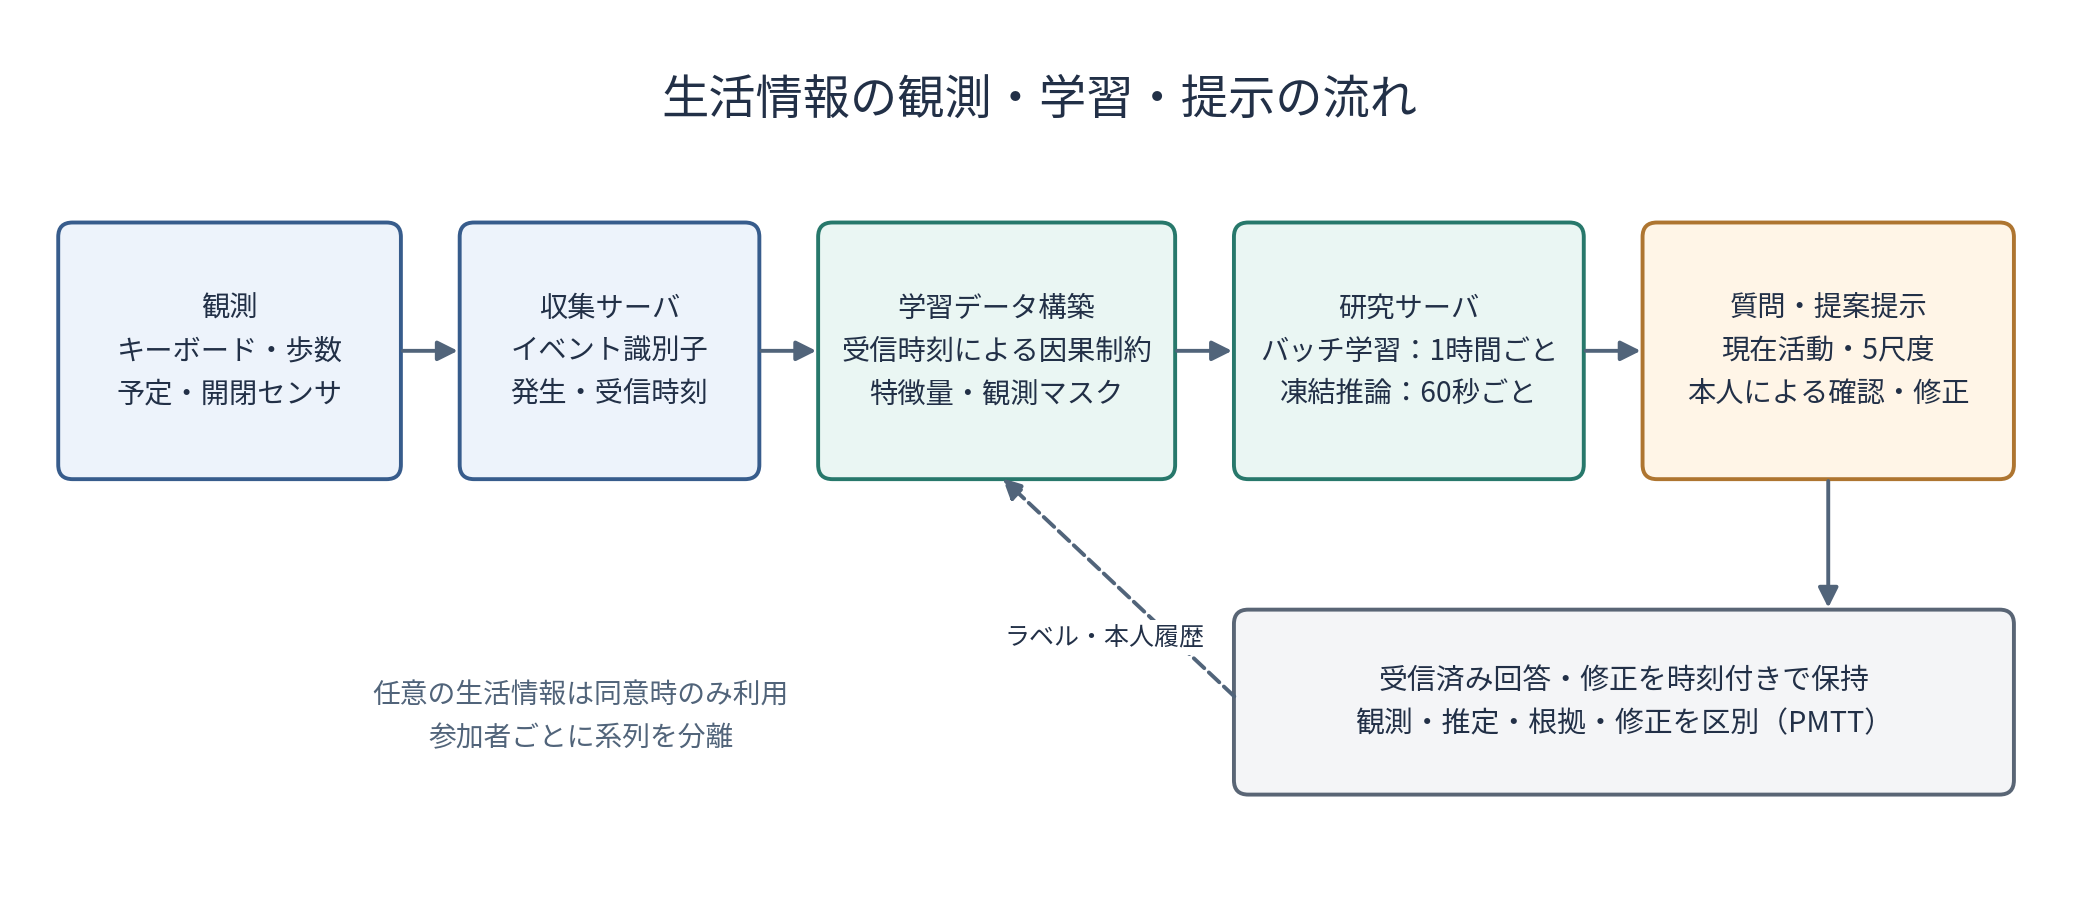
\includegraphics[width=\linewidth]{figures/fig_system_overview.png}
  \caption{従来構成の観測収集、受信時刻を保つ学習データ構築、固定活動・5尺度の推定と質問・提案提示、本人履歴とPMTTの対応。共有三階層LSTMによるPlace・Behaviorの発見を表す図ではない。}
  \label{fig:legacy-system}
\end{figure}

\chapter{共有三階層LSTMによる生活パターン発見と状態推定}
\label{chap:model}

同じ「勉強・研究」という活動名でも、文章を書く時間と実験装置を操作する時間では、観測される入力行動や生活情報が異なる。一方、場所が変わっただけで同じ作業を別の行動とみなすことも適切ではない。固定カテゴリによる活動分類と、個人固有のタスク推定を並行して行うと、何を別の状態として識別するかが二重に定義される。

本研究の提案構成では、活動の意味カテゴリをあらかじめ24個に固定せず、共有の時系列表現から拠点と行動パターンを扱う。現在・日次の5尺度も同じエンコーダから推定する。行動候補の発見、本人による同一性の確認、名前の付与は別の操作である。特徴が似た観測のまとまりが得られても、そのまとまりを直ちに「修論執筆」などの意味へ置き換えない。

対応する実装は\texttt{life-discovery-v1}である。24クラス分類を含む従来のHierarchicalLSTMと、独立したContextLSTMは比較条件として保持するが、提案構成と同時に二重の行動推定を行うものではない。実参加者における有効性は第\ref{chap:evaluation}章の評価課題であり、以下の数理的定義と実装の対応を、推定性能の検証とは分けて記述する。

\section{推定対象と観測情報}
\label{sec:prediction-targets}

参加者\(p\)について、イベント発生時刻と受信時刻の双方が推定時刻\(t\)以下である観測の集合を\(\mathcal H_p^{\rm obs}(t)\)とする。入力\(x_{p,d,u,k}\in\mathbb R^{98}\)は、33個の観測値、対応する33個の存在指示、32次元の文章特徴からなる。\(d\)は日、\(u\)は日内区間、\(k\)は区間内ビンを表す。観測値の欠測と実測ゼロを区別し、文章特徴はローカルで生成する。

本人の活動回答、拠点・行動確認、モデル推定を観測特徴にしない。24活動の回答は入力区間の境界にも用いない。入力系列を構成するTimelineには観測記録だけを渡し、質問の回答内容を変えただけで同じ観測系列の表現が変わることを防ぐ。

数式中の入力\(x\)は前処理後の特徴とする。33観測値の平均と標準偏差は訓練側の観測済み座標だけから求め、標準化後も欠測座標を存在指示でゼロ化する。存在指示と文章32座標は標準化しない。文章特徴はローカルSentenceTransformerで生成した文埋め込みを固定ランダム射影したものであり、エンコーダの同一性をcheckpointと照合する。文エンコーダの導入・比較条件は§\ref{sec:sentence-encoder}に示す。

共有エンコーダの出力を現在表現\(C_p(t)\in\mathbb R^{48}\)と日次表現\(D_p(t)\in\mathbb R^{48}\)とし、推定対象を次式で表す。

\[
\left(z_p^{P}(t),z_p^{B}(t),\hat y_p^{\rm cur}(t),\hat y_p^{\rm day}(t)\right)
=f_\theta\left(\mathcal H_p^{\rm obs}(t)\right).
\]

\(f_\theta\)はパラメータ集合\(\theta\)を持つ共有エンコーダと各出力層を合わせた写像である。\(z^P,z^B\in\mathbb R^{32}\)はそれぞれPlaceとBehaviorの表現であり、32種類の場所・行動を意味しない。\(\hat y^{\rm cur},\hat y^{\rm day}\in[1,5]^5\)は現在・日次の尺度予測ベクトルで、5尺度の順序は気分、疲労、ストレス、集中度、眠気に固定する。尺度は本人回答に対応する研究上の推定対象であり、診断や客観的な心理状態の測定ではない。

Placeは本人が区別する生活拠点、Behaviorは本人固有の行動パターンである。同一場所の別作業と、別場所の同じ作業を独立に確認できるよう、両軸のIDを分離する。既存APIの\texttt{task}および\texttt{taskCheck}はBehaviorの互換名として維持し、第三の推定対象は作らない。

\section{三階層の時間表現}

各階層には隠れ次元48の単方向LSTMを一つずつ用いる。LSTMの基本更新はゲートを介したセルの保持と更新である\autocite{hochreiter1997lstm}。本実装で用いる忘却ゲートはLSTMの後の発展に対応する\autocite{gers2000forget}。階層を\(\ell\in\{\mu,m,M\}\)とし、順にMicro、Meso、Macroを表す。階層内の時刻添字を\(j\)、入力を\(v_j^\ell\in\mathbb R^{d_\ell}\)、隠れ状態とセル状態を\(h_j^\ell,c_j^\ell\in\mathbb R^{48}\)とする。入力次元は\(d_\mu=98\)、\(d_m=d_M=48\)である。各階層のゲート更新を次式で定義する。

\[
\begin{aligned}
i_j^\ell&=\sigma(W_i^\ell v_j^\ell+U_i^\ell h_{j-1}^\ell+b_i^\ell),&
f_j^\ell&=\sigma(W_f^\ell v_j^\ell+U_f^\ell h_{j-1}^\ell+b_f^\ell),\\
o_j^\ell&=\sigma(W_o^\ell v_j^\ell+U_o^\ell h_{j-1}^\ell+b_o^\ell),&
g_j^\ell&=\tanh(W_g^\ell v_j^\ell+U_g^\ell h_{j-1}^\ell+b_g^\ell),\\
c_j^\ell&=f_j^\ell\odot c_{j-1}^\ell+i_j^\ell\odot g_j^\ell,&
h_j^\ell&=o_j^\ell\odot\tanh(c_j^\ell).
\end{aligned}
\]

\(i_j^\ell,f_j^\ell,o_j^\ell\in(0,1)^{48}\)は入力・忘却・出力ゲート、\(g_j^\ell\in(-1,1)^{48}\)はセルへ書き込む候補である。\(\sigma(a)=1/(1+\exp(-a))\)と\(\tanh\)は各座標へ適用し、\(\odot\)は要素積を表す。ゲート種別\(\gamma\in\{i,f,o,g\}\)ごとに、\(W_\gamma^\ell\in\mathbb R^{48\times d_\ell}\)は入力重み、\(U_\gamma^\ell\in\mathbb R^{48\times48}\)は再帰重み、\(b_\gamma^\ell\in\mathbb R^{48}\)はバイアスである。実装の入力側・再帰側バイアスは式の\(b_\gamma^\ell\)へ合算して表す。したがってMicroでは98次元の観測を、MesoとMacroでは48次元の下位表現を、同じ形式のゲートで48次元の記憶へ更新する。重みは階層別に持ち、PlaceとBehaviorごとに別の三階層を作るものではない。

入力ゲートは候補情報の書込み、忘却ゲートは過去セルの保持、出力ゲートは隠れ状態への読出しを制御する。これらのゲートは学習されるため、時間尺度ごとの固定平滑化係数ではない。セルの加法的経路は記憶の保持を助けるが、長期依存を常に学習できることを保証しない。

\subsection{MicroとMeso}

以下では同一参加者の推定を記述するため、参加者添字\(p\)と推定時刻\(t\)を必要な箇所以外で省略する。Microは正時境界で区切った最大1時間を、最大12個の5分ビンとして処理する。末尾の短いビンは実際の長さで構成し、推定時刻より後の観測を含めない。日\(d\)の区間\(u\)における有効ビン数を\(K_{d,u}\)とする。Microのゲート式に\(v_k^\mu=x_{d,u,k}\)を代入し、区間ごとの初期状態を\((h^\mu_{d,u,0},c^\mu_{d,u,0})=(0,0)\)として順に更新する。区間の最終隠れ状態\(w_{d,u}\in\mathbb R^{48}\)は

\[
w_{d,u}=h^\mu_{d,u,K_{d,u}}
=\operatorname{LastHidden}\left(\operatorname{LSTM}_{\mu}(x_{d,u,1:K_{d,u}})\right)
\]

である。\(\operatorname{LastHidden}\)はパディングを除いた系列の最終隠れ状態を返す操作、\(1:K_{d,u}\)は最初から有効長までの系列を表す。Mesoは日\(d\)の有効区間数\(U_d\)に対して\(v_u^m=w_{d,u}\)を入力し、\((h^m_{d,0},c^m_{d,0})=(0,0)\)から時間順に更新する。日表現\(q_d\in\mathbb R^{48}\)は

\[
q_d=h^m_{d,U_d}
=\operatorname{LastHidden}\left(\operatorname{LSTM}_{m}(w_{d,1:U_d})\right)
\]

である。保存テンソルは一日48区間を上限とし、有効長を別に保持する。提案構成では活動回答による追加分割を行わない。過去日はその日の終端まで、当日は推定時刻までの観測を使う。過去日の観測でも、受信が推定時刻に間に合っていることを要求する。

実装は有効長の系列をパックし、パディングを無操作の実測ビンとしてLSTMへ与えない。長さゼロの保存区間の表現はゼロとする。ちょうど日付が変わった時点には空の部分ビンを一つ設け、有効長を扱えるようにする。推定時刻が区間途中であれば、その時点までの部分系列の最終状態を使うため、区間終了後の情報を待ってから現在予測を行う構成ではない。

\subsection{Macroと融合}

当週は日本標準時の月曜日開始とする。当週開始前に対応する28個の日別観測特徴\(r_i\in\mathbb R^{98}\)を古い順に線形射影し、当週の日表現列へ時間方向に連結する。\(r_i\)にも第\ref{chap:observations}章の訓練側統計による前処理を適用する。過去28日は保存されたMesoの隠れ状態ではなく、日別観測を再集約した特徴である。当週開始を\(W\)とすると、履歴窓は\((W-(i+1)\text{日},W-i\text{日}]\)、\(i=27,\ldots,0\)である。下式の\(r_1\)は\(i=27\)の最古窓、\(r_{28}\)は\(i=0\)の最新窓に対応する。右閉区間であるため、\(W\)ちょうどのイベントは最後の履歴窓に含まれる。受信締切はいずれの窓でも推定時刻\(t\)である。

推定時刻が属する当週の日添字を\(d_*\)、当日の現在区間添字を\(u_*\)とする。当週の日は古い順に\(1,\ldots,d_*\)と数える。履歴の射影行列とバイアスを\(W_H\in\mathbb R^{48\times98}\)、\(b_H\in\mathbb R^{48}\)とし、Macroの入力\(v_j^M\)を次式で定義する。

\[
v_j^M=
\begin{cases}
W_Hr_j+b_H,&1\le j\le28,\\
q_{j-28},&29\le j\le28+d_*.
\end{cases}
\]

Macroは\((h^M_0,c^M_0)=(0,0)\)から上記のゲート式を\(28+d_*\)ステップ適用する。その最終隠れ状態\(H\in\mathbb R^{48}\)は

\[
H=h^M_{28+d_*}
=\operatorname{LastHidden}\left(\operatorname{LSTM}_{M}
\left([W_Hr_1+b_H,\ldots,W_Hr_{28}+b_H,q_1,\ldots,q_{d_*}]\right)\right).
\]

となる。日次表現\(D\in\mathbb R^{48}\)と現在表現\(C\in\mathbb R^{48}\)は次式で得る。

\[
D=\tanh(W_D[q_{d_*};H]+b_D),\qquad
C=\tanh(W_C[w_{d_*,u_*};D;H]+b_C).
\]

\(W_D\in\mathbb R^{48\times96}\)、\(W_C\in\mathbb R^{48\times144}\)は融合行列、\(b_D,b_C\in\mathbb R^{48}\)はバイアスである。\([\cdot;\cdot]\)は特徴方向の連結であり、Macro式中の列は時間方向の連結である。実装の\texttt{top\_day}が\(D\)、\texttt{top\_work}が\(C\)に対応する。

\subsection{階層間の状態の受渡し}

時間方向の状態更新と階層間の受渡しを区別するため、階層\(\ell\)のゲート式全体を写像\(\Phi_\ell\)と表す。下位の最終隠れ状態が上位の一入力となる関係は、次式にまとめられる。

\[
\begin{aligned}
(h^\mu_{d,u,k},c^\mu_{d,u,k})
&=\Phi_\mu(x_{d,u,k},h^\mu_{d,u,k-1},c^\mu_{d,u,k-1}),\\
(h^m_{d,u},c^m_{d,u})
&=\Phi_m(w_{d,u},h^m_{d,u-1},c^m_{d,u-1}),\\
(h^M_j,c^M_j)
&=\Phi_M(v_j^M,h^M_{j-1},c^M_{j-1}).
\end{aligned}
\]

Microのセル\(c^\mu\)は区間内の記憶であり、Mesoへ渡す\(w_{d,u}\)はその読出しである。同様に、Mesoのセル\(c^m\)をMacroへ移すのではなく、日表現\(q_d\)を入力する。したがって三階層のセルは互いに独立した48次元の記憶を持ち、下位の細かな系列を上位の時間単位へ要約する。逆方向には\(H\)と\(D\)を融合式へ渡し、現在表現\(C\)を文脈で条件付ける。上位の文脈はMicroのセルへ直接注入しない。

現行実装は各系列を初期状態から再計算する。推論間のhidden/cell持越しや、本番のTBPTTによる逐次重み更新は含まない。条件付き状態保持を行う比較計画の切断長と保存・復元規則は§\ref{sec:legacy-ssl-and-adaptation}で定義する。表現の受渡し、LSTM内部状態の持越し、離散状態IDの時間遷移はそれぞれ異なる操作であり、最後の時間遷移は§\ref{sec:pattern-discovery}のグラフとして扱う。

\section{拠点・行動・主観尺度の出力}

PlaceとBehaviorは共通の現在表現から別の射影を通して得る。\(W_P,W_B\in\mathbb R^{32\times48}\)は軸別の射影行列、\(b_P,b_B\in\mathbb R^{32}\)はそのバイアスである。任意のベクトル\(v\)について\(\operatorname{norm}(v)=v/\max(\lVert v\rVert_2,\epsilon)\)、\(\epsilon=10^{-12}\)とすれば、

\[
z^P=\operatorname{norm}\{\tanh(W_PC+b_P)\},\qquad
z^B=\operatorname{norm}\{\tanh(W_BC+b_B)\}.
\]

射影後の\(\tanh\)は座標の大きさを制限し、正規化前のノルムが\(\epsilon\)以上なら、正規化後の内積をコサイン類似度として比較できる。文章特徴の32次元化は凍結した固定射影であるのに対し、この二つの\(48\to32\)射影は共有エンコーダとともに学習する。入力文章の32次元と出力の32次元は、座標の意味や重みを共有しない。極小ノルムによる正規化の例外はマップ入力時に再検査する。

現在・日次の尺度は別の出力層で推定する。\(W_{\rm cur},W_{\rm day}\in\mathbb R^{5\times48}\)と\(b_{\rm cur},b_{\rm day}\in\mathbb R^5\)をそれぞれ尺度出力の重みとバイアスとすると、

\[
\hat y^{\rm cur}=1+4\sigma(W_{\rm cur}C+b_{\rm cur}),\qquad
\hat y^{\rm day}=1+4\sigma(W_{\rm day}D+b_{\rm day}).
\]

となる。右辺の定数1は5座標へ加え、各尺度の出力を本人回答の1〜5の範囲へ写す。Place・Behaviorは現在表現\(C\)から、日次尺度は日次表現\(D\)から得るため、日次尺度を現在尺度の単純平均として定義しない。

5尺度の予測値を行動クラスタリングの距離へ連結しない。この構成は、出力得点の変化だけによって直接別の行動ノードへ割り当てることを避ける。ただしエンコーダは共有されるため、行動表現から心理状態の影響が完全に除去されるわけではない。

同様に、射影を二つ設けるだけでは場所と行動の意味は分離されない。自宅でしか行わない作業は、自宅を示す観測と共起し続ける。両者を区別するための情報は、異なる場所で同じ行動を行った観測、同じ場所で別行動を行った観測、および独立した本人確認である。観測上区別できない状態は不明のまま残す。

\section{自己教師あり学習と本人確認の併用}
\label{sec:joint-learning}

学習は自己教師あり損失と本人回答の損失を同時に最適化する。別段階の事前学習を必須とする構成ではない。教師がない観測からも表現を学習するが、無回答を架空の正解として補わない。

\subsection{マスク再構成と将来予測}

非空のバッチを\(\mathcal B\)、その件数を\(n_{\mathcal B}=|\mathcal B|\)とし、例\(i\in\mathcal B\)の最新有効ビンを\(x_i\in\mathbb R^{98}\)とする。以下の添字\(j\)はこの最新ビンの特徴座標である。基礎量の座標集合を\(\mathcal J_v=\{1,\ldots,33\}\)、文章座標集合を\(\mathcal J_e=\{67,\ldots,98\}\)とする。基礎量のうち時間周期、区間長、heartbeat鮮度、収集設定の座標集合を\(\mathcal J_{\rm ex}\subset\mathcal J_v\)とし、これらは再構成対象から除外する。文章長\texttt{text\_chars}の基礎量座標を\(j_{\rm text}\in\mathcal J_v\)、基礎量\(j\)の元の存在指示を\(m_{i,j}\)とする。元の観測有効性\(\omega_{i,j}\)を

\[
\omega_{i,j}=
\begin{cases}
m_{i,j},&j\in\mathcal J_v\setminus\mathcal J_{\rm ex},\\
m_{i,j_{\rm text}},&j\in\mathcal J_e,\\
0,&\text{その他}
\end{cases}
\]

と定義する。座標34〜66のpresence自体は予測の正解にしない。観測済みの基礎量ごとに独立な選択変数\(\xi_{i,j}\sim\operatorname{Bernoulli}(0.2)\)を抽選し、文章には例ごとに一つの\(\xi_i^{\rm text}\sim\operatorname{Bernoulli}(0.2)\)を抽選する。\(\operatorname{Bernoulli}(0.2)\)は確率0.2で1、それ以外で0を返す分布である。\(j\in\mathcal J_e\)では\(\xi_{i,j}=\xi_i^{\rm text}\)とし、対象外の座標では\(\xi_{i,j}=0\)とする。選択された有効座標集合は

\[
\mathcal M=
\{(i,j):i\in\mathcal B,\ \omega_{i,j}=1,\
\xi_{i,j}=1,\ x_{i,j}\text{が有限}\}
\]

である。基礎量を隠すときは値\(x_{i,j}\)と対応するpresence \(x_{i,33+j}\)をともに0にする。文章は32座標全体を一つのブロックとして隠す。マスク後の現在表現から元の特徴を再構成し、\(\mathcal M\)だけに損失を適用する。

文章ブロック自体の選択確率も0.2であり、32座標を独立に抽選してからブロックへ拡張する旧SSLの方式とは異なる。文章を隠すときは\texttt{text\_chars}の値と存在指示も消す。ただし文章長座標を\(\mathcal M\)へ含めるかは、その基礎量自身の抽選による。非マスク入力の出力を将来予測・関係・尺度・分散損失に用い、再構成だけにはマスク入力からの別の順伝播を用いる。例\(i\)のマスク後の現在表現を\(C_i^{\rm mask}\in\mathbb R^{48}\)とし、\(W_{\rm rec}\in\mathbb R^{98\times48}\)と\(b_{\rm rec}\in\mathbb R^{98}\)を再構成ヘッドの重みとバイアスとすると、\(\hat x_i=W_{\rm rec}C_i^{\rm mask}+b_{\rm rec}\)である。

\[
\mathcal L_{\rm rec}=\frac{\sum_{(i,j)\in\mathcal M}(\hat x_{i,j}-x_{i,j})^2}{\max(1,|\mathcal M|)}.
\]

再構成の正解は標準化後の元の最新ビンである。\(|\mathcal M|\)は有効座標数であり、集合が空の場合は損失を0とする。将来予測は64次元の\([z^P;z^B]\)から次の1時間\((t,t+1\text{時間}]\)の観測特徴を推定する。例\(i\)の予測時刻を\(t_i\)、1時間後の終端を\(t_i^+=t_i+1\text{時間}\)、当該分割の教師締切を\(T_i^{\rm split}\)、データ取得締切を\(T_{\rm acq}\)とする。将来教師を利用できる指示を

\[
\gamma_i^+=\mathbf1\{t_i^+<T_i^{\rm split},\ t_i^+\le T_{\rm acq}\}
\]

と定義する。将来区間の生特徴を訓練側統計で変換した教師を\(\tilde x_i^+\in\mathbb R^{98}\)とし、その区間の観測有効性\(\omega_{i,j}^+\)を\(\omega_{i,j}\)と同じ座標規則で求める。将来教師マスクは\(m_{i,j}^+=\gamma_i^+\omega_{i,j}^+\mathbf1[\tilde x_{i,j}^+\text{が有限}]\)である。\(W_+\in\mathbb R^{98\times64}\)と\(b_+\in\mathbb R^{98}\)を将来予測ヘッドの重みとバイアスとして、

\[
\hat x_i^+=W_+[z_i^P;z_i^B]+b_+,\qquad
\mathcal L_{\rm future}=\frac{\sum_{i,j}m_{i,j}^+(\hat x_{i,j}^+-\tilde x_{i,j}^+)^2}{\max(1,\sum_{i,j}m_{i,j}^+)}
\]

とする。和は\(i\in\mathcal B\)と\(j=1,\ldots,98\)について取り、有効でない座標は和から除く。将来損失には隠す座標の抽選を行わず、予測対象として有効な観測座標すべてを用いる。各損失は例ごとの平均をさらに平均するのではなく、バッチ全体の有効座標で平均する。予測対象の1時間の終端が分割の締切以上、またはデータ取得締切より後である場合は、そのターゲットを使わない。将来特徴はその終端までに受信された観測から作る教師であり、現在入力へ渡すものではない。この条件により、再構成は現在の観測間の関係、将来予測は次の1時間に関わる表現を学習する。

\subsection{本人確認による関係学習}

軸\(a\in\{P,B\}\)ごとに、例\(i\)で本人が確認した正規IDを\(k_i^a\)とする。ここでの添字\(i,j\)はともにバッチ内の例であり、特徴座標ではない。別名解決後の本人確認IDを双方が持つペア集合\(\mathcal P_a=\{(i,j):i,j\in\mathcal B,\ j<i,\ k_i^a,k_j^a\text{が有効}\}\)を作る。\(j<i\)によって各組を一度だけ数える。正規化された埋め込みの内積\((z_i^a)^\top z_j^a\)を類似度とし、同一IDの表現は近づけ、異なるIDは類似度が0.3を超える場合に離す。

\[
\ell_a(i,j)=
\begin{cases}
1-(z_i^a)^\top z_j^a,& k_i^a=k_j^a,\\
\max\{0,(z_i^a)^\top z_j^a-0.3\},& k_i^a\ne k_j^a,
\end{cases}
\qquad
\mathcal L_{\rm rel}^{a}=\frac{\sum_{(i,j)\in\mathcal P_a}\ell_a(i,j)}{\max(1,|\mathcal P_a|)}.
\]

\(\ell_a(i,j)\)は一組の関係損失、\(\mathcal L_{\rm rel}^a\)は有効ペア間の平均である。同一IDの項は類似度1で0になり、異なるIDの項は類似度0.3以下では0になる。異なるIDをすべて反対方向へ押し離す制約ではない。Placeの正解をTaskの違いから生成することも、その逆も行わない。未確認、わからない、移動中には同一性ラベルを作らない。命名だけの操作も同一性の教師を追加しない。

\subsection{尺度損失と全体損失}
\label{sec:scale-and-total-loss}

現在・日次の尺度には回答済み有限値の座標だけのHuber損失を用いる\autocite{huber1964robust}。scopeを\(s\in\{\mathrm{cur},\mathrm{day}\}\)、尺度添字を\(j=1,\ldots,5\)、例\(i\)に対応する本人回答を\(y_{i,j}^s\)とする。有効回答マスクを\(m_{i,j}^{y,s}=\mathbf1[y_{i,j}^s\text{が回答済みの有限値で }1\le y_{i,j}^s\le5]\)とし、有効な例と尺度の組を\(\mathcal O_s=\{(i,j):i\in\mathcal B,\ m_{i,j}^{y,s}=1\}\)とする。残差を\(r=\hat y_{i,j}^{s}-y_{i,j}^{s}\)、閾値1のHuber関数を\(\rho_1\)とすれば、

\[
\mathcal L_s=\frac{\sum_{(i,j)\in\mathcal O_s}\rho_1(\hat y_{i,j}^{s}-y_{i,j}^{s})}{\max(1,|\mathcal O_s|)},\qquad
\rho_1(r)=\begin{cases}\tfrac12r^2,&|r|<1,\\|r|-\tfrac12,&|r|\ge1.\end{cases}
\]

となる。残差の絶対値が1未満では二乗誤差、1以上では線形に増えるため、大きい残差の寄与を二乗誤差より抑える。未回答座標は補完せず、分母にも含めない。

埋め込みが単一の値へ縮退することを抑えるため、各軸にバッチ内分散のペナルティも加える。軸\(a\)の埋め込み座標\(j=1,\ldots,32\)について、バッチ平均を\(\bar z_j^a\)、母分散を\(V_j^a\)とすると、

\[
\bar z_j^a=\frac1{n_{\mathcal B}}\sum_{i\in\mathcal B}z_{i,j}^a,\qquad
V_j^a=\frac1{n_{\mathcal B}}\sum_{i\in\mathcal B}
(z_{i,j}^a-\bar z_j^a)^2
\]

である。\(n_{\mathcal B}\ge2\)の場合、分散損失を

\[
\mathcal L_{\rm var}^{a}=\frac1{32}\sum_{j=1}^{32}
\max\{0,0.05-\sqrt{V_j^a+10^{-4}}\}
\]

とする。0.05は各座標の標準偏差に対する下限、\(10^{-4}\)は平方根内の安定化定数である。\(V_j^a\)はバッチ件数で除した分散であり、不偏分散ではない。バッチが一例の場合、\(\mathcal L_{\rm var}^a=0\)とする。回答のない尺度損失と有効ペアのない関係損失もゼロとし、欠測を架空の教師に置き換えない。尺度損失は現在・日次ごとに有効座標で平均するため、一方の回答数の多さだけで他方を希釈しない。全体は次式である。

\[
\mathcal L=\mathcal L_{\rm rec}+\mathcal L_{\rm future}
+\mathcal L_{\rm cur}+\mathcal L_{\rm day}
+0.1\sum_{a\in\{P,B\}}\mathcal L_{\rm rel}^{a}
+0.1\sum_{a\in\{P,B\}}\mathcal L_{\rm var}^{a}.
\]

24クラスの交差エントロピーは含めない。分散項や関係損失は表現の制約であり、意味の分離を保証する定理ではない。既定の最適化はAdamW\autocite{loshchilov2019adamw}、学習率0.001、weight decay0.001、バッチ8、12エポック、乱数seed37、勾配ノルム上限1である。AdamWのweight decayは損失への単純なL2項の加算と区別する。観測例は各エポックでシャッフルし、LSTMの状態は例間で引き継がない。

再構成、将来予測、現在尺度、日次尺度の係数は各1であり、関係損失と分散損失の係数0.1はPlace・Behaviorのそれぞれに掛かる。全体損失\(\mathcal L\)の勾配は共有エンコーダへ集まり、再構成ヘッドには再構成項、将来ヘッドには将来項、各尺度ヘッドには対応する尺度項が伝わる。この同時最適化によって、観測の構造と本人の確認・回答を共通の時系列表現へ反映する。

\section{カテゴリ数を固定しないパターン発見}
\label{sec:pattern-discovery}

DiscoveryMapは、閾値に基づく逐次プロトタイプマップに、有向の時間遷移グラフを付したものである。プロトタイプの幾何学的な近さと、時間的に隣接した状態への変更を別々に記録する。ノード数はデータと本人確認に応じて変わり、24活動の数に拘束されない。

\subsection{プロトタイプ割当てと更新アルゴリズム}

軸\(a\in\{P,B\}\)のノードID集合を\(\mathcal V^a\)とし、ノード\(j\in\mathcal V^a\)に、代表ベクトル\(c_j^a\in\mathbb R^{32}\)、割当て件数\(n_j^a\in\mathbb N_0\)、本人確認の有無\(b_j^a\in\{0,1\}\)を保持する。\(\mathbb N_0\)は0以上の整数の集合である。プロトタイプ集合は\(\mathcal C^a=\{c_j^a:j\in\mathcal V^a\}\)、全ノード数は\(K_a=|\mathcal V^a|\)である。別名から正規IDを返す写像を\(\operatorname{can}_a\)とし、未知または未確認IDの欠如を\(\bot\)で表す。未確認候補数とその容量を

\[
K_{\rm unc}^a=\sum_{j\in\mathcal V^a}(1-b_j^a),\qquad
B_{\max}=256
\]

と定義する。この上限は未確認候補に適用し、本人確認済みのIDを含む全ノード数の上限とはしない。

アルゴリズムの入力は、訓練側の観測から固定したモデルで得る時刻順の組\((t_\nu,z_\nu^a,k_\nu^a)\)である。\(\nu\)は観測の処理順、\(t_\nu\)は割当て対象時刻、\(z_\nu^a\)は軸別埋め込み、\(k_\nu^a\)は訓練締切までに利用できる本人確認IDであり、確認がなければ\(\bot\)とする。全座標が有限で\(\lVert z_\nu^a\rVert_2>10^{-8}\)であることを検査し、マップ内で再正規化した\(\zeta_\nu^a=z_\nu^a/\lVert z_\nu^a\rVert_2\)を用いる。零ベクトル・極小ノルム・非有限値はエラーとする。代表も単位長なので、コサイン類似度と勝者は

\[
s_{\nu j}^a=(\zeta_\nu^a)^\top c_j^a,\qquad
j_\nu^*=\operatorname*{arg\,max}_{j\in\mathcal V^a}s_{\nu j}^a,\qquad
s_\nu^*=s_{\nu j_\nu^*}^a
\]

である。同点の場合はIDの順で決定する。\(\mathcal V^a=\varnothing\)なら\(j_\nu^*=\bot\)、\(s_\nu^*=-\infty\)とする。受入れ閾値を\(\tau=0.88\)とし、割当てID\(a_\nu\)を次式で定める。

\[
a_\nu=
\begin{cases}
\operatorname{can}_a(k_\nu^a),&k_\nu^a\ne\bot,\\
j_\nu^*,&k_\nu^a=\bot,\ s_\nu^*\ge\tau,\\
\operatorname{newID}_a(t_\nu),&
k_\nu^a=\bot,\ s_\nu^*<\tau,\ K_{\rm unc}^a<B_{\max},\\
\bot,&\text{その他}.
\end{cases}
\]

\(\operatorname{newID}_a(t_\nu)\)は当該軸と時刻から新候補の識別子を作る操作であり、固定活動番号を返すものではない。本人確認IDへの割当てを類似度より優先する第1分岐は、訓練側のマップ構築にだけ用いる。これを含む構築手順は次のとおりである。

\begin{enumerate}
\def\labelenumi{\arabic{enumi}.}
\item
  同一モデルで再符号化した既知IDの元観測をアンカーとして読み込み、代表\(c_j^a\)を初期化する。アンカーはIDに対応する元観測であり、旧モデルの重心ではない。アンカーの件数は\(n_j^a=0\)とする。確認済みアンカーを先に確保し、未確認アンカーには候補容量を適用する。
\item
  各\(t_\nu\)を厳密な昇順で処理し、上の割当て式を適用する。\(a_\nu=\bot\)なら代表を更新せず、時間辺を作るための直前割当てを消去して次へ進む。
\item
  \(a_\nu\notin\mathcal V^a\)なら、\(c_{a_\nu}^a=\zeta_\nu^a\)、\(n_{a_\nu}^a=0\)でノードを作る。本人確認IDの新規作成では\(b_{a_\nu}^a=1\)、新候補では0とする。確認済みIDは未確認候補の容量によって拒否しない。
\item
  割当て先\(j=a_\nu\)に次の再帰更新を適用し、本人確認があれば\(b_j^a=1\)とする。観測日と確認日も区別して記録する。
\item
  §\ref{sec:transition-graph}の条件で時間辺の回数を更新し、現在の割当てを次の直前割当てとして保持する。
\end{enumerate}

手順4の更新で用いる中間ベクトルを\(v_j^a=n_j^ac_j^a+\zeta_\nu^a\)とすると、

\[
c_j^a\leftarrow
\begin{cases}
v_j^a/\lVert v_j^a\rVert_2,&\lVert v_j^a\rVert_2>10^{-8},\\
\zeta_\nu^a,&\text{その他},
\end{cases}
\qquad n_j^a\leftarrow n_j^a+1
\]

である。新規ノードおよびアンカーは件数0で初期化するため、最初の割当てで代表はその埋め込みへ更新される。更新ごとに正規化するため、全埋め込みの単純な算術平均と同一ではなく、従来GrowingMapの欠測に応じた座標別平均（§\ref{sec:legacy-growingmap}）とも異なる。

上限時に十分近い代表がない観測は\(\bot\)となり、最寄りへ強制割当しない。本人確認済みのIDを候補数の上限だけで削除しない。本方式は閾値型の逐次プロトタイプ法であり、関連研究としてのGrowing Neural Gasの誤差蓄積、第2勝者や近傍の更新、辺の加齢・削除、誤差に基づく挿入則を実装したものではない。GNGとの相違と従来マップの数理は§\ref{sec:legacy-growingmap}および§\ref{sec:legacy-transition-ratios}に整理する。

\subsection{時間遷移グラフと推論時の固定}
\label{sec:transition-graph}

ここでは軸を\(\alpha\in\{P,B\}\)、辺の始点・終点IDを\(a,b\)と書き、軸とノードの添字を区別する。時間遷移グラフを\(\mathcal G^\alpha=(\mathcal V^\alpha,\mathcal E^\alpha,N^\alpha)\)とし、\(N_{ab}^\alpha\in\mathbb N_0\)を状態変更回数、\(\mathcal E^\alpha=\{(a,b):a\ne b,\ N_{ab}^\alpha>0\}\)を有向辺集合とする。回数はマップ再構築時に0から集計する。実装はPlaceとBehaviorの両マップに辺を持つが、生活パターンの提示にはBehaviorのマップを用いる。

軸ごとの直前割当てを\(\pi^\alpha=(a,t_{\rm prev})\)または\(\bot\)とし、最初は\(\bot\)とする。現在の割当てが\(b\)、時刻が\(t_\nu\)で、\(\pi^\alpha\ne\bot\)の場合の時間差を\(\Delta t=t_\nu-t_{\rm prev}\)と定義する。隣接した有効割当ての増分条件は

\[
N_{ab}^{\alpha}\leftarrow N_{ab}^{\alpha}
+\mathbf1\{a\ne b,\ 0<\Delta t\le1\text{時間}\}
\]

である。現在が未知なら\(\pi^\alpha\leftarrow\bot\)とし、辺を加えない。有効割当てなら、時間差が1時間を超えて辺を加えない場合も含めて\(\pi^\alpha\leftarrow(b,t_\nu)\)とする。この手順によって、長い未観測区間や候補上限による未知区間を跨いで辺を作らない。自己遷移は数えず、同じノードが続く場合にも直前時刻を更新する。

保存・表示する辺の量は回数であり、同一状態への滞在を含む次観測の遷移確率ではない。例えば\(a,a,b\)という系列では、\(a\)での滞在は辺を増やさず、時間条件を満たす\(a\to b\)だけを1回数える。従来構成の状態変更率\(Q_{ab}\)（§\ref{sec:legacy-growingmap}）と同様に、仮に変更回数から構成比を導出しても「記録された状態変更の内訳」である。従来の12時間という接続条件は新方式に流用しない。

マップ全体の保存状態を\(\mathscr M^\alpha\)とし、プロトタイプ、件数、確認属性、別名、時間辺の回数を含める。検証・テスト・ライブ推論で埋め込み\(z^\alpha\)を受け取るときは、同じ正規化と順位付けによる勝者\(j^*\)と最大類似度\(s^*\)を求め、候補IDを

\[
\hat k^\alpha=
\begin{cases}
j^*,&\mathcal V^\alpha\ne\varnothing,\ s^*\ge0.88,\\
\bot,&\text{その他}
\end{cases},
\qquad
(\theta,\mathscr M^\alpha)_{\rm after}
=(\theta,\mathscr M^\alpha)_{\rm before}
\]

とする。下付き\(\rm before,after\)は一回の推論の前後を表す。本人確認IDによる優先割当てはこの推論式には入れず、候補IDと正解IDを独立に比較できるようにする。新ノード生成、代表更新、件数加算、時間辺加算を推論時には行わない。類似度が閾値を満たしても、モデル推定として表示するにはさらに§\ref{sec:confirmation-and-estimation}の支持条件を必要とする。

マップの構築は訓練側データだけで行い、新しい候補の反映は次回のバッチ再学習時である。埋め込みが変わったときには、既知IDの元観測を新モデルで再符号化し、古い重心を新しい特徴空間へ混ぜない。離散状態IDの系列とその時間辺は、三階層LSTMが生成した表現を事後に割り当てたものであり、上位LSTMのセル状態そのものではない。

\section{意味付けと候補・推定の区別}
\label{sec:confirmation-and-estimation}

24活動の本人回答は、モデルとマップを固定した後に、対応する行動ノードの説明件数として集計する。一つのノードに複数の活動名が対応してよく、活動名の追加でノード数や重心を変えない。この集計は提案モデルの学習損失でも、別の24クラス予測器でもない。評価区間の注釈を用いて事前の対応表を作ることは避ける。

意味の命名と機械の推定は分けて保存する。例えば未確認候補に「修論執筆」と本人が命名した場合、その名称は本人による解釈であり、クラスタリングだけで自動獲得した意味ではない。場所や文章特徴だけから実際の作業を確定しない。

本人が対象区間のIDを確認した記録は\texttt{confirmed}、\texttt{source=self\_report}として扱う。これと、モデルが凍結マップへ割り当てた\texttt{candidate}、割当てに至らない\texttt{unknown}、表示条件を満たすモデル推定\texttt{estimated}、\texttt{source=model}を区別する。候補ノードが本人確認を持つことと、新しい区間のIDを本人が確認したことも同一ではない。本人確認表示とモデル推定の一致は評価対象であり、一方を他方へ自動変換しない。

ライブでIDを推定表示する初期条件は、本人確認の支持が2日以上、軸の検証が2件以上かつID一致率0.5以上、最大類似度0.88以上、次候補との差0.08以上である。単一候補の場合や、本人確認・統合が更新されて未学習の場合は断定しない。閾値は探索的設定で、コサイン類似度を校正された確率と解釈しない。

各尺度は学習10回答・検証3回答に満たない項目の数値を表示しない。未学習、推定時刻から遡って1時間以内に終了してその時刻までに受信されたセッションがない場合、将来時点で学習されたモデル、異なる文章エンコーダの利用も推定停止条件とする。heartbeatや開閉センサの周期観測だけでは、このセッションの鮮度条件を満たさない。確認質問の選択に用いる同日3時間の条件（§\ref{sec:context-confirmations}）によって、推論の1時間条件が緩和されることもない。これらの下限は表示を抑制する条件であり、精度保証ではない。

\section{検証・運用と従来構成の位置付け}
\label{sec:legacy-and-deployment}

\subsection{時系列分割と候補モデルの検証}

直近28日の観測から最大240時点を選び、最低12時点・3日を要求する。日単位の時系列順で約65\%を訓練、20\%を検証、15\%をテストとする。各分割にはその締切までに受信した教師だけを使う。本人回答時点の追加後に480時点を超える場合はエラーとし、黙って切り捨てない。正規化統計は訓練側だけで求める。

検証では将来特徴予測のマスク付き二乗誤差と、有効な現在・日次尺度のHuber損失の和を比較する。正規化が異なる候補モデルと現行モデルも、同じ検証時点・同じ誤差尺度へ戻して比較する。テスト成績をモデル昇格へ使わない。ID一致率や尺度別MAEも保存するが、提示された正解IDが少ないことを考慮して解釈する。

検証目的関数には再構成・関係・分散の各損失を加えない。各エポックの候補をこの目的関数で選び、適合する現行\texttt{life-discovery-v1}モデルがある場合には同じ検証集合で比較し、候補が悪化しない場合に昇格する。ここでの現行モデルとの比較は、従来の24活動分類器との研究上の比較とは異なる。テストは明示実行時だけ集計し、昇格へ用いない。

\subsection{方式選択と保存・提示}
\label{sec:runtime-selection}

新構成は\texttt{research\_architecture=discovery}として明示選択し、従来構成を\texttt{legacy}として保持する。現在・日次・拠点・行動を一つのcheckpointから推論し、独立ContextLSTMの学習ワーカーは起動しない。旧checkpoint、元データ、回答、命名を削除せず、保存先を分離する。後日の振り返りは再解析時刻とモデルIDを持つ別記録とし、当時のライブ推定を上書きしない。

サーバー設定の既定は\texttt{legacy}である。提案方式の学習では、従来方式とは別の\path{discovery/}保存先に候補・有効・旧版のcheckpointを保持する。CLIは単一参加者の完全なexportと、方式の由来を確認できる出力先を要求し、旧checkpointのディレクトリへ上書きしない。

新しい状態IDに基づく歩数基準と介入の検証は未完了である。このため、新構成では旧状態マップに依存する歩数保存・運動提案、および旧疲労推定に依存する提案判定を動かさない。5尺度の推定と候補の確認・命名・訂正は維持する。生活パターンが得られることと、それに基づく支援が有効であることは別の検証対象である。

% 追加: 従来breakCheckとlive時のDiscovery支援経路を区別する。
一方、LSTMとは別の\texttt{typing\_change}と本人の訂正理由を使う質問経路は新構成にも残る。質問予算を4枠より増やした場合、訂正率の変化に対する\texttt{typingReason}を選択できる。\texttt{discovery\_support\_mode}が\texttt{off}または\texttt{shadow}の場合、質問予算等の条件を満たすと、入力訂正の変化と直近2時間の\texttt{mistype}回答に基づく従来の\texttt{breakCheck}を選択できる。\texttt{live}ではこの従来提案を抑止し、Discoveryの支援判断と事前・事後評価を用いる別経路を選択する。既定4枠ではこれらのイベント質問を選択せず、22時以降は日次回答を優先する。この補助経路は新しいBehavior IDや5尺度推定の有効性に基づく支援ではなく、休憩提案がすべての設定で無効になったという説明とも区別する。

\subsection{従来構成：固定活動分類と個人履歴条件付け}

以下は\texttt{legacy}に属する従来構成と独立した比較・拡張の記述である。固定24活動分類、独立した拠点・Task推定、生観測GrowingMap、本人回答履歴の条件付けを、新方式の追加の推定器や入力経路として組み込まない。

従来HierarchicalLSTMは三階層表現から24活動の確率と、現在・日次5尺度を出力する。活動出力には履歴条件付け後の現在表現\(C'\in\mathbb R^{48}\)を用い、\(\pi=\operatorname{softmax}(W_AC'+b_A)\in\mathbb R^{24}\)とする。\(W_A\in\mathbb R^{24\times48}\)と\(b_A\in\mathbb R^{24}\)は活動出力層の重みとバイアスであり、\(\pi_c\)は活動\(c\)の出力確率である。

別のContextLSTMは拠点とTaskを推定し、その階層の隠れ次元の既定値は24である。提案する共有エンコーダの隠れ次元48と混同しない。従来のTaskは独立モデルの対象であり、新方式におけるBehaviorの通信互換名\texttt{task}とはモデル上の役割が異なる。従来方式では活動回答・訂正の利用可能な境界で区間を追加分割するが、新方式の観測系列ではこれを行わない。

\begin{figure}[tbp]
  \centering
  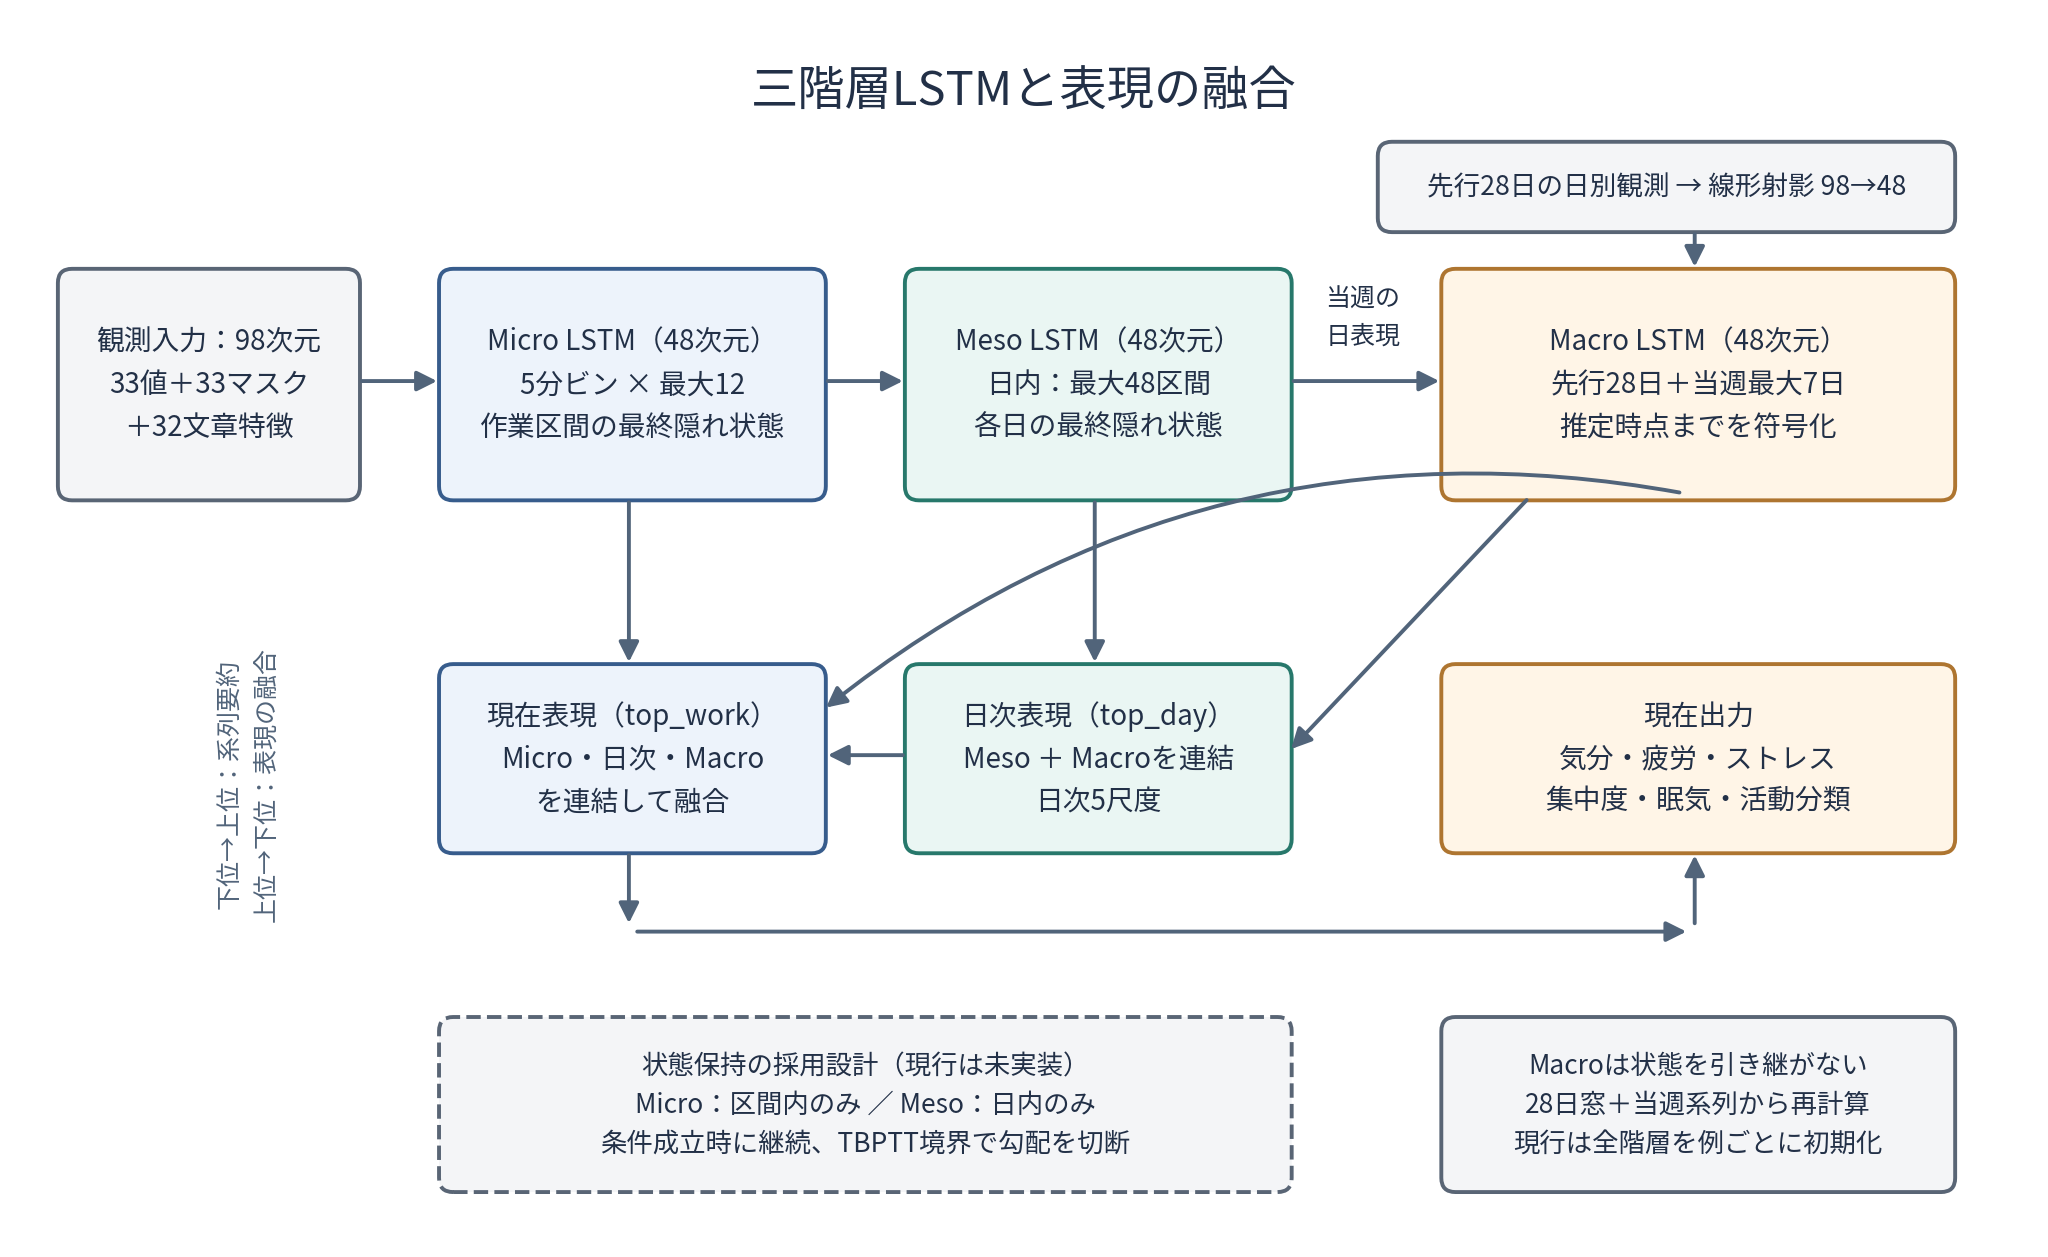
\includegraphics[width=\linewidth]{figures/fig_hierarchical_lstm.png}
  \caption{固定活動分類を持つ従来HierarchicalLSTMの図である。現在出力の「活動分類」は新方式には存在しない。下段の状態保持・TBPTTは従来の比較設計の注記であり、運用実装はいずれの方式でも系列ごとに初期化する。本図を新方式のPlace/Behavior射影と同時学習の検証資料として用いない。}
  \label{fig:legacy-lstm}
\end{figure}

従来の本人履歴条件付けは、本人の過去回答の平均を表現へ加える操作である。参加者\(p\)、予測時刻\(t\)、回答対象\(s\in\{\mathrm{cur},\mathrm{day}\}\)に対し、回答記録\(e\)の参加者を\(p_e\)、回答対象を\(s_e\)、対象時刻を\(t_e^{\rm target}\)、受信時刻を\(t_e^{\rm recv}\)、尺度\(j\)の回答を\(y_{ej}\)、有限かつ有効な回答が存在する指示を\(m_{ej}\in\{0,1\}\)とする。\(j=1,\ldots,5\)は§\ref{sec:prediction-targets}の尺度順序に対応する。全履歴、同時刻帯、同曜日、同活動の四群を表す群集合を\(\mathcal G\)とする。

\[
\mathcal G=\{\mathrm{all},\mathrm{hour},\mathrm{weekday},\mathrm{activity}\}.
\]

既存の群判定に従って回答\(e\)が時点\(t\)の群\(g\)に属するかを\(\chi_g(e;t)\in\{0,1\}\)とし、\(\chi_{\rm all}(e;t)=1\)とする。

同時刻帯は日本標準時の同じ時刻の「時」、同曜日は同じ曜日への一致である。\(\operatorname{hour}\)と\(\operatorname{weekday}\)をそれぞれ時と曜日を返す関数、\(a_e\)を回答\(e\)に対応する既存活動ID、\(a(t)\)を推定時刻までに利用可能な対象時点の既存活動IDとすると、

\[
\begin{aligned}
\chi_{\rm hour}(e;t)
&=\mathbf1\{\operatorname{hour}(t_e^{\rm target})=\operatorname{hour}(t)\},\\
\chi_{\rm weekday}(e;t)
&=\mathbf1\{\operatorname{weekday}(t_e^{\rm target})=\operatorname{weekday}(t)\},\\
\chi_{\rm activity}(e;t)
&=\mathbf1\{a(t)\text{が有効},\ a_e=a(t)\}.
\end{aligned}
\]

活動IDが未知のときは同活動群への一致を作らない。

\[
\begin{aligned}
\mathcal A_{pgj}^{s}(t)
&=\{e:p_e=p,\ s_e=s,\ t_e^{\rm target}<t,\
t_e^{\rm recv}<t,\ m_{ej}=1,\ \chi_g(e;t)=1\},\\
n_{pgj}^{s}(t)&=|\mathcal A_{pgj}^{s}(t)|,\qquad
\bar y_{pgj}^{s}(t)=
\frac1{n_{pgj}^{s}(t)}
\sum_{e\in\mathcal A_{pgj}^{s}(t)}y_{ej}
\quad\bigl(n_{pgj}^{s}(t)>0\bigr).
\end{aligned}
\]

四群は互いに排他的ではなく、一回答が複数群の平均に寄与してよい。件数が3件以上の群・尺度だけを有効とし、平均20個と存在指示20個を40次元特徴\(\phi_p^{s}(t)\)へまとめる。各群では5尺度の平均を先に、その後に5尺度の存在指示を並べ、四群をall、hour、weekday、activityの順に連結する。この順序は学習と推論で固定する。

\[
\begin{aligned}
v_{pgj}^{s}(t)&=\mathbf1\{n_{pgj}^{s}(t)\ge3\},\\
a_{pgj}^{s}(t)&=
\begin{cases}
\bar y_{pgj}^{s}(t),&v_{pgj}^{s}(t)=1,\\
3,&v_{pgj}^{s}(t)=0,
\end{cases}\\
\phi_p^{s}(t)&=
[a_{pg1}^{s}(t),\ldots,a_{pg5}^{s}(t),
v_{pg1}^{s}(t),\ldots,v_{pg5}^{s}(t)]_{g\in\mathcal G}
\in\mathbb R^{40},\\
P_p^{s}(t)&=\tanh(W_{\rm hist}\phi_p^{s}(t)+b_{\rm hist})
\in\mathbb R^{48},\\
C'^{\,s}&=C+P_p^{s}(t),\qquad D'^{\,s}=D+P_p^{s}(t).
\end{aligned}
\]

\(W_{\rm hist}\in\mathbb R^{48\times40}\)と\(b_{\rm hist}\in\mathbb R^{48}\)は履歴射影の学習パラメータであり、\(P_p^{s}(t)\)は履歴による条件付け表現である。補完値3は存在指示ゼロによって実測平均と区別する。current用とdaily用では利用する回答集合が異なるため、それぞれの履歴特徴を与えた順伝播から対応する出力層の値を採用する。一回の順伝播の内部では、同じ条件付け表現を現在・日次の双方へ加える。

同じ群判定の下で新たに利用可能となった回答値\(y\)を一件加えるとき、件数\(n\)と平均\(\bar y\)の更新は\(n^+=n+1\)、\(\bar y^+=\bar y+(y-\bar y)/n^+\)である。\(n=0\)なら\(\bar y^+=y\)で初期化する。ここで上付き\(+\)は追加後の統計を表す。この更新は回答統計の更新であり、モデル重みの更新ではない。予測時刻によって時刻帯等の群判定が変わる場合は、対象集合を選び直す。

条件付けは推論中の重み更新ではなく、過去56日の条件付きベースラインによる「普段との差」とも異なる。新方式ではこの40次元変換をモデルから除いている。従来基本モデルのパラメータ数86,050は固定24活動ヘッドと履歴条件付けを含む値であり、新方式のパラメータ数として用いない。

従来の教師損失は、活動例の交差エントロピーに係数0.2を掛け、現在または日次の尺度例には有効座標のHuber平均を用い、有効例間で平均する。活動例と尺度例を一例ごとに区別するこの集約は、§\ref{sec:joint-learning}の新方式で現在・日次の有効座標をそれぞれ平均する集約とは異なる。従来基本モデルはバッチ4、AdamW、学習率0.001・weight decay0.001、勾配ノルム上限1を用い、尺度の検証平均MAEで候補を選ぶ。

\subsection{従来構成：生観測GrowingMapと状態変更率}
\label{sec:legacy-transition-ratios}

従来GrowingMapはLSTMの隠れ状態をクラスタリングせず、10分の非重複打鍵窓から生観測特徴を作る。20 inserts以上の窓に対して挿入量の対数、訂正率、休止率、時刻の正弦・余弦を用いる。保存済み\texttt{context\_inference}のうち窓終端から10分以内で、受信が推定時刻に間に合い、拠点・Task両IDを持つ最も近い記録を対応させる。対応記録がなければラベルは未知とする。本人回答と文脈モデル推定の情報源を区別し、名称ではなく別名解決後の識別子で照合する。

観測座標集合\(O_z\)と中心\(i\)の観測座標集合\(O_i\)の共通部分\(J_i\)に対し、同じ拠点・Taskの識別子対を持ち、\(|J_i|\ge3\)の場合だけ

\[
d_i(z)=\sqrt{\frac1{|J_i|}\sum_{j\in J_i}(z_j-a_{ij})^2}
\]

を使い、それ以外は距離を\(+\infty\)とする。最小距離が半径\(\rho=0.35\)以内なら勝者へ割り当て、観測された座標だけを座標別回数\(n_{ij}\)による逐次平均で更新する。

\[
n'_{ij}=n_{ij}+1,\qquad
a'_{ij}=a_{ij}+\frac{z_j-a_{ij}}{n'_{ij}}\quad(j\in O_z).
\]

初めて観測した座標は回数1、値\(z_j\)とし、欠測座標は保持する。中心の接近による統合も座標別回数の加重平均で行い、同一ラベル・共通座標3以上・距離\(\rho/2\)以下を条件とする。古いIDを残し、削除IDを別名として解決し、端点を正規IDへ集約して自己辺を除く。これが従来構成の座標平均であり、新方式の正規化埋め込みの再帰更新とは異なる。

観測特徴が3以上で既存中心がないか距離が半径を超え、ノード数が256未満なら新ノードを生成する。上限到達後の遠い観測を最寄りへ強制割当しない。従来の状態変更回数と、その回数から導く構成比は

\[
\begin{aligned}
N_{ab}&\leftarrow N_{ab}+\mathbf1\{a\ne b,\ 0\le\Delta t\le12\text{時間}\},\\
Q_{ab}&=\frac{N_{ab}}{\sum_{c\ne a}N_{ac}}
\quad\left(b\ne a,\ \sum_{c\ne a}N_{ac}>0\right).
\end{aligned}
\]

である。\(Q_{ab}\)はAから記録された状態変更のうちBへ移った割合であり、Aへの滞在を含む次観測の遷移確率ではない。分母0なら未定義とし、保存対象は回数\(N_{ab}\)である。距離半径0.35と12時間の条件は新方式へ引き継がない。GrowingMapにも新方式にもGNGの誤差蓄積、第2勝者・近傍の更新、辺の加齢・削除則はなく、GNGの再現とは呼ばない\autocite{fritzke1995gng}。従来マップの処理図と詳細は§\ref{sec:legacy-growingmap}に示す。

\subsection{従来構成・比較計画：SSL、部分プーリングと逐次適応}
\label{sec:legacy-ssl-and-adaptation}

従来の\texttt{research/ssl.py}は、マスク再構成と5〜30分先の観測特徴予測で事前学習し、その後に固定活動分類・尺度の教師で微調整する二段階の実験経路である。マスク予測や再構成の一般的背景としてBERTとMasked Autoencodersを参照する\autocite{devlin2019bert,he2022mae}。従来SSLでは文章32座標のどれかを初期確率\(q=0.2\)で選んだ場合にブロック全体を隠すため、文章ブロックの選択確率は\(1-(1-q)^{32}\)である。新方式の最新ビンにおける文章ブロックの選択確率0.2とは異なる。

従来SSLは区間表現・日表現・Macro表現からの観測再構成、28日履歴再構成、将来予測のマスク付き二乗損失を係数1で合成する。将来教師のホライズンは5・10・15・20・25・30分から設定し、既定は5・15・30分である。SSL中は本人履歴をゼロ化し、固定活動・尺度ヘッド、履歴条件付け、個人バイアスを更新しない。事前学習後に補助ヘッドを外し教師付き学習へ進む。訓練カットオフより前の将来教師だけを使い、入力側のみから正規化統計を求める。§\ref{sec:joint-learning}の最新ビン再構成と次1時間予測を教師損失と同時に学ぶ構成へ、この旧機構を流用しない。

部分プーリングの独立実験経路\texttt{ExperimentalModel}は、実験内の共有エンコーダと参加者別の5次元バイアス\(b_p\)を用い、現在・日次に同じバイアスを加える\autocite{gelman2007multilevel}。参加者\(p\)の例\(e\)の観測入力を\(x_e\)、回答対象を\(s_e\)、尺度\(j\)の回答値を\(y_{ej}\)、回答マスクを\(m_{ej}\)とする。\(f_\theta^s(x_e)\in\mathbb R^5\)は共有重み\(\theta\)による回答対象\(s\)の尺度出力、\(n_{pj}\)は初期訓練および当該逐次更新までに取り込んだ参加者\(p\)・尺度\(j\)の回答数である。\(\tau>0\)はガウス事前の標準偏差、\(I\)は5次元単位行列、\(\lambda_b=10\)は収縮係数を表す。

\[
\begin{aligned}
\hat y_{p,e}^{s}&=f_\theta^{s}(x_e)+b_p,\qquad
b_p\sim\mathcal N(0,\tau^2I),\\
\ell_e^{\rm pool}
&=\frac1{\sum_{j=1}^5m_{ej}}
\sum_{j=1}^5m_{ej}
\left[
(f_\theta^{s_e}(x_e)_j+b_{pj}-y_{ej})^2+
\frac{\lambda_b b_{pj}^2}{\max(n_{pj},1)}
\right],
\quad \sum_{j=1}^5m_{ej}>0.
\end{aligned}
\]

ガウス事前は収縮罰則の解釈であり、事後分布を計算する実装ではない。尺度損失はHuberではなく二乗誤差で、活動には係数0.2付き交差エントロピーを用いる。参加者バイアスへのAdamW weight decayはゼロとし、明示的な収縮を二重適用しない。シグモイド出力後にバイアスを加えるため、出力は1〜5を超え得て、現行実験ではクリップしない。未登録参加者のバイアスはゼロとする。全参加者共通の完成済みグローバルモデルが配布されていることを前提とせず、新方式へ部分プーリングを追加済みとも解釈しない。

prequential比較では、各参加者の予測値と更新に用いた回答数を、対象の回答を受信する前に保存し、その後届いた教師で採点する。参加者\(p\)の予測時刻列を\(t_1<t_2<\cdots\)、時刻\(t_k\)で過去回答による更新を行う前の参加者内モデル重みを\(\theta_{p,k,0}\)、観測入力を\(x_p(t_k)\)とする。\(\mathcal U_{p,k}\)はそれまでの逐次更新に使った回答ID集合であり、最初は空集合とする。参加者内モデルの初期訓練締切を\(T_p^{\rm tr}\)とし、初期訓練期間の回答を再び新規教師として使わない。更新用回答集合\(\mathcal A_{p,k}\)には、締切以後の対象時刻で、予測より厳密に前に対象時刻と受信時刻の双方があり、まだ更新に使っていない有効回答だけを含める。

\[
\begin{aligned}
\mathcal A_{p,k}
&=\{e:p_e=p,\ T_p^{\rm tr}\le t_e^{\rm target}<t_k,\ t_e^{\rm recv}<t_k,\
\mathrm{id}_e\notin\mathcal U_{p,k},\ e\text{が有効教師例}\}.
\end{aligned}
\]

ここで\(p_e\)、\(\mathrm{id}_e\)、\(t_e^{\rm target}\)、\(t_e^{\rm recv}\)は回答の参加者、識別子、対象時刻、受信時刻を表す。この集合を受信順に並べ、同時刻の場合は対象時刻等の保存キーで順序を固定して、回答を一件ずつ更新へ用いる。予測後に到着した回答は時刻\(t_k\)の更新集合へ遡って追加せず、以後の予測時点で条件を満たしたときに利用する。

従来参加者内モデルの全層微調整では、活動例と尺度例を区別した損失\(\ell_e^{\rm online}\)を用いる。活動例の正解カテゴリを\(a_e\in\{1,\ldots,24\}\)、予測確率を\(\pi_{e,a_e}\)、尺度例の回答対象を\(s_e\)、有効尺度数を\(M_e=\sum_{j=1}^5m_{ej}\)とする。\(\rho_1\)は§\ref{sec:scale-and-total-loss}の閾値1のHuber関数である。

\[
\ell_e^{\rm online}=
\begin{cases}
-\log\pi_{e,a_e},&e\text{が活動例},\\
\displaystyle\frac1{M_e}\sum_{j=1}^5
m_{ej}\rho_1(\hat y_{ej}^{s_e}-y_{ej}),
&e\text{が尺度例},\ M_e>0.
\end{cases}
\]

\(\mathcal A_{p,k}\)を並べた列を\((e_1,\ldots,e_{R_{p,k}})\)、その長さを\(R_{p,k}=|\mathcal A_{p,k}|\)とする。回答\(e_r\)を使う直前の重みは\(\theta_{p,k,r-1}\)である。勾配\(g_{p,k,r}=\nabla_{\theta_{p,k,r-1}}\ell_{e_r}^{\rm online}\)を計算する。勾配ノルムの上限1に合わせて\(\operatorname{clip}_1(g)=g/\max(1,\|g\|_2)\)と定義し、一件ごとの更新と予測保存を次式で表す。

\[
\begin{aligned}
\theta_{p,k,r}
&=\operatorname{AdamW}_{\eta}(\theta_{p,k,r-1},\operatorname{clip}_1(g_{p,k,r})),
\quad
\eta=0.0001,\quad r=1,\ldots,R_{p,k},\\
\hat y_{p,k}
&=f_{\theta_{p,k,R_{p,k}}}(x_p(t_k)),\qquad
\theta_{p,k+1,0}=\theta_{p,k,R_{p,k}},\\
\mathcal U_{p,k+1}
&=\mathcal U_{p,k}\cup\{\mathrm{id}_e:e\in\mathcal A_{p,k}\}.
\end{aligned}
\]

\(\operatorname{AdamW}_{\eta}\)は当該参加者の最適化状態を保持する学習率\(\eta\)のAdamW更新を表す。活動交差エントロピーには通常学習の係数0.2を掛けない。更新集合が空なら重みと使用済みID集合を保持する。保存した\(\hat y_{p,k}\)を後の重みで再計算しない。参加者\(p\)の回答で他参加者の従来参加者内モデルを更新しない。

この更新演算を明示するため、参加者\(p\)の通算更新番号を\(q\ge1\)とし、その更新に対応するノルム制限後の勾配を\(\bar g_{p,q}=\operatorname{clip}_1(g_{p,k,r})\)、更新後の重みを\(\theta_p^{(q)}\)と書く。勾配の一次・二次モーメントを\(m_{p,q}^{\rm opt},v_{p,q}^{\rm opt}\)とし、初期値はともに0である。\(\beta_1,\beta_2\in[0,1)\)はモーメントの減衰係数、\(\epsilon_{\rm opt}>0\)は分母の安定化定数、\(\lambda_{\rm wd}\ge0\)はweight decay係数であり、最適化の設定として記録する。AdamW演算は

\[
\begin{aligned}
m_{p,q}^{\rm opt}
&=\beta_1m_{p,q-1}^{\rm opt}+(1-\beta_1)\bar g_{p,q},\\
v_{p,q}^{\rm opt}
&=\beta_2v_{p,q-1}^{\rm opt}
+(1-\beta_2)(\bar g_{p,q}\odot\bar g_{p,q}),\\
\hat m_{p,q}^{\rm opt}
&=\frac{m_{p,q}^{\rm opt}}{1-\beta_1^q},\qquad
\hat v_{p,q}^{\rm opt}=\frac{v_{p,q}^{\rm opt}}{1-\beta_2^q},\\
\theta_p^{(q)}
&=(1-\eta\lambda_{\rm wd})\theta_p^{(q-1)}
-\eta\frac{\hat m_{p,q}^{\rm opt}}
{\sqrt{\hat v_{p,q}^{\rm opt}}+\epsilon_{\rm opt}}
\end{aligned}
\]

である。\(\hat m^{\rm opt},\hat v^{\rm opt}\)は初期値0による偏りを補正したモーメントであり、平方根とベクトル間の除算は座標ごとに行う。モーメントと通算番号\(q\)は予測時点が変わっても保持する。weight decayは適応的な勾配項と別に重みへ作用するため、損失へ二乗罰則を足す更新と区別する。

部分プーリングのFrozen・Biasのみ適応・全層適応の三条件は別経路である。比較条件ごとに共有重みと全参加者のバイアスを独立に複製し、そのパラメータを\(\psi=(\theta,\{b_p\}_p)\)とする。この経路では使用済み集合を初期訓練例のキーで初期化し、対象時刻・受信時刻が予測より厳密に前という条件と、未使用という条件で回答を選ぶ。参加者内モデルの対象時刻下限をそのまま追加せず、初期訓練で未使用の遅延回答も利用条件で判定する。共有モデルの比較では参加者ごとの回答を同じ受信順の列へまとめる。回答\(e\)による更新の直前と直後のパラメータを\(\psi^{-},\psi^{+}\)とする。更新目的\(\ell_e^{\rm comp}\)には、尺度例なら\(\ell_e^{\rm pool}\)、活動例なら係数0.2付き交差エントロピーを用いる。更新する座標を選ぶ指示ベクトル\(v_e\)を用いると、

\[
\psi^{+}
=\psi^{-}-\eta\,\operatorname{clip}_1
\left(v_e\odot\nabla_{\psi^{-}}\ell_e^{\rm comp}\right)
\]

である。Frozenでは\(v_e\)の全座標を0、Biasのみ適応では回答者\(p_e\)の\(b_{p_e}\)の座標のみ1、全層適応では全学習パラメータの座標を1とする。同一学習率のSGDを用い、momentumとweight decayは加えない。Biasのみ適応では他参加者のバイアス行を保持し、全層適応では共有重みも変化する。使用済み回答のキーは参加者、回答ID、回答対象の組とする。これらは評価用の逐次適応条件であり、ライブ推論のオンライン学習を実装したという主張ではない。

適応条件では尺度回答\(e\)を損失へ渡す前に、回答者の件数を\(n_{p_ej}^{+}=n_{p_ej}^{-}+m_{ej}\)と更新し、収縮項の分母には追加後の件数を使う。上付き\(-,+\)は当該回答を取り込む直前・直後を表す。Frozen条件の件数と重みは保持する。

状態保持型TBPTTは独立の比較計画である\autocite{williams1990tbptt}。階層\(\ell\in\{\mu,m\}\)の系列を、最大\(L_\ell\)ステップのチャンクへ分ける。\(L_\mu\)はMicroの5分ビン数、\(L_m\)はMesoの区間表現数による切断長であり、\(1\le L_\mu\le12\)、\(1\le L_m\le48\)の整数とする。これらの上限は既存の系列上限から与えるもので、固定の既定切断長は現行本文・実装で定められていないため、比較実験の条件として両値を記録する。

階層\(\ell\)の有効系列長を\(J_\ell>0\)、チャンク番号を\(r=1,\ldots,\lceil J_\ell/L_\ell\rceil\)とすると、チャンク\(r\)の実際の長さは\(\min\{L_\ell,J_\ell-(r-1)L_\ell\}\)である。末尾の短いチャンクでは、有効系列の残りだけを処理する。

チャンク\(r\)の最終隠れ状態と最終セル状態を\(h_{\ell,r}^{\rm end},c_{\ell,r}^{\rm end}\in\mathbb R^{48}\)とする。\(r\)はチャンク番号であり、次チャンク冒頭への引継ぎ指示\(\gamma_{\ell,r}\in\{0,1\}\)が1である場合だけ、値を保存して勾配を切る。

\[
\begin{aligned}
(h_{\ell,r+1}^{\rm init},c_{\ell,r+1}^{\rm init})
&=
\begin{cases}
(\operatorname{stopgrad}(h_{\ell,r}^{\rm end}),
\operatorname{stopgrad}(c_{\ell,r}^{\rm end})),
&\gamma_{\ell,r}=1,\\
(0,0),&\gamma_{\ell,r}=0,
\end{cases}\\
\frac{\partial h_{\ell,r+1}^{\rm init}}
{\partial h_{\ell,r}^{\rm end}}&=0,\qquad
\frac{\partial c_{\ell,r+1}^{\rm init}}
{\partial c_{\ell,r}^{\rm end}}=0.
\end{aligned}
\]

\(\operatorname{stopgrad}\)は数値を保持し、前チャンクへの勾配だけを遮断する演算である。Microでは同一参加者・モデル版・日・作業区間の連続処理、Mesoでは同一参加者・モデル版・日内の連続処理に限って\(\gamma_{\ell,r}=1\)とする。Microは作業区間を処理するセッションの境界で、Mesoは日付境界で初期化する。ここでセッションとはモデルが処理する同一作業区間を指し、端末から届く個々のキーボードsession記録の境界とは区別する。参加者変更、意味境界、長い欠測、モデル版変更、処理時刻の逆行ではいずれも初期化する。

チャンク終了時には、参加者、モデル版、階層、対象の日・区間等を識別するキー、最終処理時刻、隠れ状態、セル状態を組として保存する。モデル版を\(\nu_{\rm model}\)とし、キーを\(\kappa_\mu=(p,\nu_{\rm model},\mu,d,u)\)、\(\kappa_m=(p,\nu_{\rm model},m,d)\)とする。チャンク\(r\)の最終処理時刻を\(t_{\ell,r}^{\rm end}\)とすれば、保存記録は

\[
\mathsf S_{\ell,r}=
(\kappa_\ell,t_{\ell,r}^{\rm end},
\operatorname{stopgrad}(h_{\ell,r}^{\rm end}),
\operatorname{stopgrad}(c_{\ell,r}^{\rm end}))
\]

である。復元はキーの一致と最終時刻より後の連続処理を確認した場合に限り、同じ観測を再処理して状態へ二重に取り込まない。区間終端ではMicroの保存状態を、日付終端ではMicro・Meso双方の保存状態を破棄する。週境界も日付境界に含まれる。Macroは隠れ状態・セル状態を持ち越さず、先行28日と当週の日表現から各回再計算する。状態値の長い保持と、勾配を伝える長さ\(L_\ell\)は別の条件である。この設計は評価予定であり、現行のバッチ学習・凍結推論とは分ける。

\subsection{従来構成：ベースライン暫定推定と切替}

従来のコールドスタート対応は、受信済みの本人平均・前回値を暫定値として表示し、項目ごとの十分な検証を得た後でLSTMへ切り替える独立経路である。有効化設定は既定で無効であり、新方式の支持不足による尺度非表示に追加する機構ではない。項目\(j\)に対し、対象時刻\(t_e\)と受信時刻\(r_e\)が予測より厳密に前の有効回答集合\(A_j(t)\)から

\[
\begin{aligned}
B_j^{\rm mean}(t)&=\frac1{|A_j(t)|}\sum_{e\in A_j(t)}y_{ej},\qquad
B_j^{\rm last}(t)=y_{e^*j},\\
e^*&=\operatorname*{arg\,max}_{e\in A_j(t)}(t_e,r_e,\mathrm{id}_e).
\end{aligned}
\]

を求める。回答ゼロなら値を出さない。受信前に保存した予測の過去MAEで平均が厳密に優れるときだけ平均を使い、同点または採点不足なら前回値を使う。暫定値には\texttt{source=baseline}、\texttt{provisional=true}、予測方法と先行回答数を付す。

同じ時系列検証回答IDでLSTMと両基準を採点する。訓練数\(N_j^{\rm tr}\)、共通検証数\(N_j^v\)、検証日数\(D_j^v\)、LSTMのMAE\(L_j\)、本人平均・前回値のMAE\(M_j,P_j\)を使い、\(B_j=\min(M_j,P_j)\)とすると、

\[
Q_j=\mathbf1\{N_j^{\rm tr}\ge10,\ N_j^v\ge10,\ D_j^v\ge3\},\qquad
W_j=\mathbf1\{Q_j=1,\ L_j\le B_j-0.1,\ L_j\le0.9B_j\}
\]

である。新規回答を含む別日の適格勝利を3回連続して満たした場合に切り替え、同じ回答や同日の再評価では連続数を進めない。日付の隣接する3日を要求する規則ではない。切替後は受信前に保存した直近10件の表示予測と両基準を同一集合で比較し、LSTMが良い基準より0.1点以上悪いという新規回答を伴う別日の判定が2回連続した場合にベースラインへ復帰する。9件以下では復帰判定をしない。閾値は切替条件であり、改善結果ではない。

回答ID、モデル・分割ID、件数・日数、MAE、閾値、連続数、source変更と理由を監査ログへ追記する。過去の予測を現在の重みで再計算して採点を代用せず、同一予測への重複回答を件数へ加えない。候補モデルの昇格と表示の切替は別判断である。暫定疲労値は疲労増加判定・休憩提案の根拠から除く。

\subsection{従来構成：状態内歩数、支援提案とPMTT}

従来の運動提案は、累積歩数の差を後側観測のGrowingMap状態\(s\)へ帰属させ、同状態・同参加者・同端末の過去日と比較する。参加者と端末を固定し、観測\(i\)の累積歩数を\(P_i\)、観測時刻を\(t_i\)、割当て状態を\(z_i\)とする。利用集合\(V\)は同じ日の非減少累積値で、観測間隔\(t_i-t_{i-1}\)が900秒以下、前観測と保存済み状態の結合が有効な対の添字集合である。日\(d\)の状態\(s\)に属する歩数を\(S_{s,d}\)として、

\[
\Delta P_i=\max(0,P_i-P_{i-1}),\qquad
S_{s,d}=\sum_{\substack{i\in V:\\z_i=s,\ \operatorname{day}(t_i)=d}}
\Delta P_i
\]

と定義する。\(\operatorname{day}\)は日本標準時の日付を返す。長い欠測中の増分を最後の状態へ一括帰属しない。現在の計測・端末文脈にも900秒以内の鮮度を要求し、当日の正の歩数増分を携帯の根拠とする。

判定時刻\(t\)の当日を\(d_0=\operatorname{day}(t)\)とし、同じ参加者・端末・状態\(s\)・仕様版の有効基準日集合を\(\mathcal D_s(t)=\{d:d<d_0,\ d\text{が有効基準日}\}\)とする。対応する歩数の列を\(\mathcal B_s(t)=(S_{s,d})_{d\in\mathcal D_s(t)}\)とし、同じ歩数の日も日ごとに一件として保持する。状態の別名は正規IDへ解決してから集計する。\(n_s(t)=|\mathcal D_s(t)|\)は基準日数であり、零歩も有効に計測された日には値として保持する。中央値\(m_s(t)\)と25パーセンタイル\(q_s(t)\)を次式で定義する。

\[
m_s(t)=\operatorname{median}\mathcal B_s(t),\qquad
q_s(t)=Q_{0.25}(\mathcal B_s(t)).
\]

\(Q_{0.25}\)は実装と同じ線形補間による標本分位点演算であり、\(q_s\)は状態\(s\)の過去日の歩数の下位25\%に対応する基準である。具体的には、昇順に並べた\(n\)個の値を\(b_{(1)},\ldots,b_{(n)}\)、分位を\(\alpha\in[0,1]\)とし、\(\xi=(n-1)\alpha\)、\(j=\lfloor\xi\rfloor+1\)、\(\lambda=\xi-\lfloor\xi\rfloor\)とおけば、\(Q_\alpha=(1-\lambda)b_{(j)}+\lambda b_{(\min(j+1,n))}\)である。\(\lfloor\cdot\rfloor\)は床関数であり、中央値も\(Q_{0.5}\)と一致する。空の列では基準を定義しない。現在までに集計された当日の歩数\(S_{s,d_0}(t)\)から、整数へ丸めた不足歩数\(D_s(t)\)と不足判定\(\mathrm{low}_s(t)\in\{0,1\}\)を求める。

\[
\begin{aligned}
D_s(t)&=\operatorname{round}
\bigl(\max\{0,m_s(t)-S_{s,d_0}(t)\}\bigr),\\
\mathrm{low}_s(t)&=
\mathbf1\{S_{s,d_0}(t)<q_s(t),\
D_s(t)\ge500,\ D_s(t)\ge0.25m_s(t)\}.
\end{aligned}
\]

\(\operatorname{round}\)は最近接整数への丸めで、等距離の場合は偶数を選ぶ。\(\mathbf1\)は条件が真のとき1となる指示関数である。三条件はすべて同時に要求する。\(n_s(t)<3\)なら判定せず、3〜4日は暫定、5日以上を正式とする。同一時間帯まで揃えた比較ではなく、当日途中と過去日の値を比較する機構である。判定条件と、歩数・携帯根拠の鮮度条件を満たした場合にのみ換算へ進む。

不足歩数を100歩/分の仮定で歩行相当時間へ変換し、参照METsの比を用いて候補活動\(a\)の時間を求める\autocite{ainsworth2011compendium,tudorlocke2019cadence}。\(T_{\rm walk}\)は歩行相当時間、\(T_a\)は丸め前の活動時間、\(\tilde T_a\)は提示する活動時間であり、いずれも単位は分である。\(\mathrm{METs}_a>0\)は活動\(a\)の参照METs値、3.0は参照歩行のMETs値とする。

\[
\begin{aligned}
T_{\rm walk}&=\frac{D_s(t)}{100},\\
3.0\,T_{\rm walk}&=\mathrm{METs}_a\,T_a,\qquad
T_a=T_{\rm walk}\frac{3.0}{\mathrm{METs}_a},\\
\tilde T_a&=\max\left(5,5\left\lceil T_a/5\right\rceil\right).
\end{aligned}
\]

\(\lceil\cdot\rceil\)は天井関数であり、活動時間は最小5分、5分単位で切り上げる。第2式はMETsと時間の積を揃える換算の仮定を明示する。実装の参照表は歩行3.0、速歩4.3、階段上り8.0、自転車6.8、ジョギング7.0、ストレッチ2.3、ラジオ体操4.0であり、既定では先頭4件を最大4候補として返す。換算は本人固有の消費エネルギーを推定するものではない。状態統合の別名解決と仕様版を保持し、異なる版の基準を混ぜない。歩数取得への同意と運動提案の有効化は独立であり、運動提案は既定で無効である。

従来の休憩提案\texttt{breakCheck}は疲労の高さ・持続的増加、または入力訂正の変化と本人の「誤入力」という確認を候補根拠とする。訂正の増加だけで疲労と断定しない。運動・休憩提案には時間帯、予定中抑止、質問間隔、日上限、停止・延期の提示条件を適用し、受諾、実行、有用性を別に記録する。現行の共通キューでは、イベント提案の選択には質問予算を4枠より増やす必要があり、提案スイッチだけをONにしても既定4枠で自動発行されるわけではない。参加者内の提示・非提示の無作為割付は追加実装を必要とする評価計画である。

PMTTは観測、推定、根拠、本人修正を分離する従来の情報設計であり、発見モデル自体ではない。概念上の四要素を\(M_{p,t}=(O_{p,t},I_{p,t},E_{p,t},R_{p,t})\)とする。\(O\)は観測、\(I\)は当時のモデルによる推定、\(E\)は推定・提案を支持する根拠、\(R\)は本人の回答・修正を表す。これらの情報と時間枠を結ぶ有向グラフを\(\mathcal G_{\rm PMTT}=(\mathcal V_{\rm PMTT},\mathcal E_{\rm PMTT})\)とし、\(\mathcal V_{\rm PMTT}\)を記録・時間枠・提案の頂点集合、\(\mathcal E_{\rm PMTT}\)を関係型を持つ辺の集合とする。

観測記録の頂点を\(o\)、推定を\(i\)、根拠を\(e\)、本人回答・修正を\(r\)、提案を\(a\)とする。また、観測\(o\)の発生時刻を含む正時区間の頂点を\(u(o)\)、その日の頂点を\(d(o)\)、月曜起点の固定週の頂点を\(w(o)\)とする。概念上の主要な接続は、

\[
\begin{aligned}
o&\xrightarrow{\rm used\ by}i,\qquad
e\xrightarrow{\rm supports}i\ \text{または}\ a,\qquad
r\xrightarrow{\rm targets}i\ \text{または}\ u(o),\\
o&\longrightarrow u(o)\longrightarrow d(o)\longrightarrow w(o)
\end{aligned}
\]

である。第1行は推定・提案の由来と修正の対象を表し、第2行はObservation、StateEpisode、Day、固定週Patternという時間枠間の階層的な所属を表す。時間枠間の辺と、§\ref{sec:pattern-discovery}のBehaviorプロトタイプ間の時間遷移辺は役割が異なる。時間枠の頂点は観測を整理する区間であり、プロトタイプの頂点は類似した表現をまとめる状態である。

従来APIは\texttt{session}、\texttt{narrative}、\texttt{correction}、\texttt{inference}等を情報源属性の異なるObservationとして包む。運動提案はExerciseProposalと\texttt{supports}関係に状態ID・仕様版、通常値、今日値、不足、基準日数、観測ID、携帯根拠とMETs換算を保持する。四種の専用ノードと全推定の完全な依存グラフを実装したという意味ではない。

修正頂点\(r_{\rm new}\)と対象への辺を加える操作は、頂点・辺集合の追記\(\mathcal V_{\rm PMTT}^{+}=\mathcal V_{\rm PMTT}\cup\{r_{\rm new}\}\)、\(\mathcal E_{\rm PMTT}^{+}=\mathcal E_{\rm PMTT}\cup\{(r_{\rm new},{\rm targets},i)\}\)と表せる。上付き\(+\)は修正追加後を表し、対象が区間の場合は辺の終点\(i\)をその区間頂点へ置き換える。元観測と当時の推定は保持する。この役割分離は、新方式でも確認・命名・訂正と再解析の扱いに継承する。一方、従来の状態内歩数と介入の根拠を新しいBehavior IDへ検証なしに接続しない。PMTTの情報モデルを保持することと、新方式による支援効果の実証は別の課題である。

\chapter{探索的予備研究の評価計画と考察観点}
\label{chap:evaluation}

未知の行動パターンが増えたことだけでは、生活理解が改善したとはいえない。場所の違いを別行動として分割している場合や、観測の欠落を新状態として扱っている場合もある。評価では、データ取得の成立、本人による同一性確認、未知の扱い、主観尺度の誤差を分けて検討する。本章は実験前の計画であり、達成した性能や介入効果を記すものではない。

\section{目的と実験条件}

従来の予備研究計画を維持し、対象は最大5名、参加期間は各14日間とする。分析単位は参加者・日・情報源・質問項目であり、多数のイベントを独立した参加者の代わりに扱わない。日常生活の取得と回答の実現可能性・負担を主評価とし、行動パターン発見、拠点同定、5尺度推定は探索的に評価する。

開始前に研究用キーボード、回答画面、停止・再開、歩数・予定・センサの任意同意を確認する。未同意情報源を欠測率の分母に含めない。サーバの質問予算の既定は4枠/日、発行間隔は60分で、Place/Behavior確認は合計1件/日まで交互に選ぶ。既定では現在尺度、お天気分、夜の日次尺度も各1件を基本とし、22時前には夜用の1枠を残す。質問の選択・表示条件を満たさない場合、実表示は4件未満となる。表示確認も回答もないまま期限切れになった発行は予算から外れるため、発行数そのものが常に4件以内とは限らない。実際に採用した設定と変更履歴を記録し、合成データは実参加者の精度評価へ混ぜない。

% 追加: 従来breakCheckとlive時のDiscovery支援経路を区別する。
新構成では旧状態マップに依存する運動提案と、旧疲労推定に基づく休憩提案判定を停止する。\texttt{discovery\_support\_mode}が\texttt{off}または\texttt{shadow}の場合、質問予算等の条件を満たすと、入力訂正の変化と直近2時間の\texttt{mistype}回答に基づく従来の\texttt{breakCheck}を選択できる。\texttt{live}ではこの従来提案を抑止し、Discoveryの支援判断と事前・事後評価を用いる別経路を選択する。既定4枠ではイベント質問を選択しない（§\ref{sec:runtime-selection}）。質問予算を増やす場合はこの経路の有効化も実験条件の変更として記録する。この段階の主評価に介入効果を含めず、従来計画にあった休憩提案の無作為化は、新しい状態・尺度に対する適格性と安全な提示条件を実装・確認した後の別研究とする。現在のコードに無作為割付が実装済みであるとは扱わない。

\section{取得の成立と回答負担}

\subsection{観測被覆と系列構築}

参加者\(p\)、日\(d\)、情報源\(s\)について、取得を有効にした区間集合を\(E_{pds}\)、取得状態を確認できた区間を\(O_{pds}\)とし、被覆率を\(|O_{pds}|/|E_{pds}|\)で求める。無操作と収集障害を区別し、heartbeatや設定履歴を併用する。ただしheartbeatは動作時の1回送信で再送しないため、その欠如を収集停止の確定として分母・分子へ反映しない。親アプリとキーボードの報告を区別し、取得状態を確認できない区間も記録する。

回答の対象時刻から因果的な入力を構築できた割合、受信遅延、重複、時刻不備、古い観測による除外を記録する。階層別の有効ビン数、区間数、観測日数も集計する。テンソルに28日分の欄があることを、28日分の観測が得られたことと同一視しない。モデルの入力98次元・共有階層の隠れ48次元という既定構成に対して、実際の有効観測数と本人確認・尺度教師数を併記し、計算可能性と情報の十分性を分けて検討する。従来基本モデルの86,050パラメータを新方式の規模として流用しない。

\subsection{質問・本人確認}

質問の候補生成、サーバ発行、端末での表示、回答を分ける。実際に表示された異なる実質問ID数\(N^{\rm shown}\)に対する有効回答ID数\(N^{\rm answered}\)の比を回答率とし、表示確認のない質問を別に扱う。同じ未回答\texttt{currentState}の再表示は新しい質問として数えず、再表示回数を別に集計する。回答の端末保存とサーバ受信も区別し、未送信の回答済みIDが再出題を抑止する条件を記録する。実回答を保存しないプレビューを除外し、Place、Behavior、現在・日次尺度、既存活動注釈を区別する。

全項目回答、部分回答、わからない、未回答、期限切れ、延期・停止を集計する。元回答と訂正の識別子を保持し、訂正を独立した追加回答として水増ししない。確認済みID数、各IDの確認日数、同じ拠点の異なる行動、同じ行動の異なる拠点が得られた件数を記録する。

回答時間は表示または入力開始から送信操作までとし、通信時間を含む受信遅延とは分ける。開始時刻がない場合は算出不能とする。時間帯別・日別の回答率と終了時の負担評価を併記する。EMAの頻度・継続期間・負担を扱う知見を参照するが、少数例の相関を質問頻度の因果効果と解釈しない\autocite{shiffman2008ema,eisele2022burden}。

\section{情報漏洩を防ぐ時間順分割}

提案実装は、観測日を時間順に約65\%/20\%/15\%へ分け、日付境界\(T_1<T_2\)を記録する。教師の対象時刻を\(t_i\)、利用可能時刻を\(r_i\)、実行時点を\(T_{\rm run}\)とすると、

\[
\begin{aligned}
\mathcal D_{\rm tr}&=\{i:t_i<T_1,\ r_i<T_1\},\\
\mathcal D_{\rm va}&=\{i:T_1\le t_i<T_2,\ r_i<T_2\},\\
\mathcal D_{\rm te}&=\{i:T_2\le t_i\le T_{\rm run},\ r_i\le T_{\rm run}\}
\end{aligned}
\]

とする。推定入力には各予測時刻までの観測だけを使い、テスト教師の後日到着を入力へ戻さない。正規化、自己教師あり学習、プロトタイプ構築、24活動注釈との事前対応集計は訓練側だけで行う。次の1時間を予測する教師は、その終端が分割の締切より厳密に前であり、実行時点以下である場合だけ使う。終端が分割境界に一致する教師も除外する。

モデル選択は検証のみで行い、テストは明示した最終評価で使う。テスト中のマップと重みは凍結する。毎回の再学習を含む運用評価を追加する場合は、予測時点より前に学習完了したcheckpointだけを使い、固定分割評価と混ぜない。後日の振り返りは再解析であり、当時のオンライン精度ではない。

Macでの受信時刻を保持した複製データによる評価は、収集サーバで利用可能だった情報に基づく。Ubuntuへの転送遅延やiOSの表示遅延を含む運用評価と区別し、固定分割の誤差から端末までの応答時間や当時の表示精度を推測しない。

旧分類器の既定分割と新方式の既定分割は一致するとは限らない。従来の評価計画の約60\%/20\%/20\%は、提案実装の約65\%/20\%/15\%とは別の条件である。比較実験では提案方式の分割を基準に共通の\(T_1,T_2\)と対象回答を明示して揃える。これを自動化する比較実行器は追加の評価実装に含める。異なる既定分割で得た二つのレポートを、そのまま手法差として比較しない。参加者間で学習を共有する追加比較を行う場合は、全参加者共通の日本時間の日付境界を用い、他参加者の未来期間も訓練へ入れない。

\section{拠点と行動パターンの評価}

\subsection{既知IDの同定と表示範囲}

PlaceとBehaviorを独立に集計する。本人確認がある評価時点について、訓練側で固定したプロトタイプから得た候補IDと正解IDの一致率を求める。正解IDが訓練側に存在しない時点を黙って除かず、既知・未知に層別する。推定表示の条件を満たさない場合も評価対象として記録する。

候補IDを返す割合、\texttt{estimated}を返す割合、未知・観測不足・未学習による抑制率を併記する。表示された少数例だけの正解率と、全評価時点での性能は別である。本人が回答した後の\texttt{confirmed}表示をモデルの正解として数えない。

現行レポートが出力するのは軸別の確認件数・ID一致率・未知件数である。以下の詳細な集計と可視化は追加の評価処理として実施する。

\subsection{未知発見・過分割・混合}

新しい意味の行動と単なる特徴変化を区別するため、評価用の本人注釈を使って、再学習で新たに生成した候補のうち独立した行動として確認された割合を調べる。逆に、新しい行動が既知ノードへ誤って吸収された件数も集計する。特徴から候補が作られたこと自体を正解と定義しない。

同一行動に複数ノードが対応する過分割率と、一つのノードへ異なる行動が混在する率を確認する。ノード数、支持日数、上限到達数、未割当数、再学習前後のID対応を記録する。任意のクラスタ番号を直接24活動の番号と照合せず、必要な意味対応は訓練側の注釈だけで確定する。

モデルが提示した候補への回答だけでは評価が誘導される可能性がある。候補表示に依存しない追加の区間確認を行う場合は、負担と同意を確認した評価手順として別に記録し、既存の質問上限を無断で増やさない。独立注釈が不足する場合、意味発見性能の主張を限定する。

\subsection{PlaceとBehaviorの分離}

同一拠点・異なる行動、および異なる拠点・同一行動の確認済み組について、対応軸の類似度とIDを比較する。場所を移しただけでBehaviorが必ず変わっていないか、作業を替えただけでPlaceが変わっていないかを調べる。片方の組合せが観測されない参加者では、その方向の分離能力は評価不能である。

埋め込みに別の射影を置いたこと、損失が減ったこと、二つの出力が異なることを意味分離の証明にしない。特定の行動と拠点が完全に共起する場合、観測から区別できない可能性を限界として報告する。

\section{現在・日次5尺度の評価}

参加者\(p\)、尺度\(k\)の有効回答マスク\(m_{ik}\)について、

\[
\operatorname{MAE}_{pk}=
\frac{\sum_{i\in\mathcal D_{{\rm te},p}}m_{ik}|\hat y_{ik}-y_{ik}|}
{\sum_{i\in\mathcal D_{{\rm te},p}}m_{ik}},\qquad
\operatorname{MAE}_{\rm macro}=\frac1{|\mathcal P_*|}\sum_{p\in\mathcal P_*}
\frac1{|\mathcal K_p|}\sum_{k\in\mathcal K_p}\operatorname{MAE}_{pk}
\]

を主指標とする。\(\mathcal K_p\)は評価可能な尺度、\(\mathcal P_*\)は評価可能な参加者であり、分母ゼロは評価不能とする。現在・日次、尺度別の値と支持件数も示す。全回答をまとめた平均だけで、回答数の多い参加者を過大に重み付けしない。

提案CLIは参加者ごとの尺度別MAEを出力する。参加者を統合したmacro値は実験集計で求める。潜在的な数値出力のオフライン誤差と、支持条件を満たして表示した時点の誤差・被覆率を区別する。14日・1日1回答程度では、学習10回答・検証3回答という表示条件へ達しないことがある。未表示を失敗として隠さず、少数データで成立する範囲の結果として記録する。

水準誤差に加え、変化方向の一致を補助的に調べる。同一参加者・同一scope（現在または日次）・同一尺度の有効回答対\(\mathcal Q_{pk}\)について、\(\operatorname{sgn}(\hat y_j-\hat y_i)=\operatorname{sgn}(y_j-y_i)\)の割合を順序一致と定義する。同値は符号0として扱い、正解の差が非0の対も別に集計する。回答対がない場合は評価不能とし、対を独立標本として有意性の標本数に用いない。この集計は追加の評価処理であり、現行CLIの自動出力とは区別する。

参照予測は訓練期間の本人平均、予測前に受信した直前回答、訓練期間の時間帯平均とする。参照予測と提案モデルを同じ時点・同じ有効マスクで比較する。自己教師あり学習の将来特徴誤差は表現学習の診断値であり、主観尺度の正確さの代替指標ではない。

\section{比較条件とアブレーション}

比較条件は、従来の24分類・5尺度モデルと独立ContextLSTM、生観測特徴を用いる旧GrowingMap、共有エンコーダと埋め込みマップを用いる提案方式とする。24分類のmacro-F1は固定分類器に対する指標である。提案方式のクラスタ番号にそのまま適用せず、事後の意味対応を評価する場合は、訓練側で固定した対応規則、未対応状態、被覆率を明示する。

従来の固定分類器については、参加者\(p\)の評価正解または予測に出現したクラス集合\(\mathcal C_p\)を用いて、

\[
\begin{aligned}
P_c &= \frac{TP_c}{TP_c+FP_c}, &
R_c &= \frac{TP_c}{TP_c+FN_c}, \\
F1_c &= \frac{2TP_c}{2TP_c+FP_c+FN_c}, &
\operatorname{macroF1}_p &= \frac1{|\mathcal C_p|}\sum_{c\in\mathcal C_p}F1_c
\end{aligned}
\]

とする。分母が0の適合率・再現率は0とし、\(\mathcal C_p\)が空なら評価不能とする。学習側に存在しなかったクラスも除外せず、混同行列、クラス別件数、accuracyを併記する。既存のaccuracyレポートからmacro-F1を推測せず、保存した予測と正解に対する追加集計として求める。

要素の寄与として、時間階層の削減、文章特徴の有無、自己教師あり再構成・将来予測の除去、本人確認による関係損失の有無を比較する計画とする。現行DiscoveryModelのCLIはこれらすべての切替を公開していないため、比較用実装と同条件の学習予算を追加してから評価する。単に旧コードにvariantが存在することを、新方式のアブレーションが完了したこととみなさない。

入力条件は、打鍵のみ、打鍵と文章特徴、打鍵・文章特徴・同意済み生活情報の三条件を基本とする。同意の異なる参加者間を直接比較せず、同一参加者内の共通時点と有効教師を使う。文章の主条件は第\ref{chap:observations}章\ref{sec:sentence-encoder}節のローカルSentenceTransformerとし、従来の基本・文脈・SSL・部分プーリングの経路と提案方式で同一のモデルrevision・内容ハッシュ・固定射影を用いる。

文字n-gramとSentenceTransformerは異なる条件として扱う。情報源を除く場合は値とpresenceの双方を無効にし、文章長などの代理特徴が残る比較と区別する。従来コードの文章ベクトルだけを0にする\texttt{no\_text}を、文章由来の全特徴を除く条件とはみなさない。乱数seed、最大エポック、時刻境界、モデル選択規則を記録し、テスト結果を見て有利な条件だけを選ばない。

状態保持型TBPTT、部分プーリング、prequentialな重み更新は別の拡張計画とする。今回の共有モデルは一参加者の系列を使ったバッチ学習であり、共通のエンコーダという語はPlace・Behavior・尺度間の共有を指す。参加者間で共同学習したモデルであるとは限らない。

従来構成の履歴条件付けの有無は重みを固定して比較し、prequential評価では予測後に受信された未使用回答だけを将来の更新へ利用する。部分プーリングの比較は凍結、個人バイアスのみ更新、全層更新を分け、加算後の尺度出力をクリップせずに誤差を求める。本人平均による暫定推定とモデルへの切替・復帰は、従来経路の監査対象として保存された回答前予測から確認する。これらを新方式のライブ推論の機構とは扱わない。

従来の二段階SSLを比較する場合は、事前学習なし、SSL後の出力層学習、上位層の微調整を、同じ実験経路の教師損失と学習予算でそろえる。新方式の再構成・次1時間予測の除去比較は同時学習に対するアブレーションであり、従来の5〜30分先予測と二段階学習をそのまま移植しない。

\section{解釈の範囲}

最大5名・14日間では、季節変化、長期習慣、未知参加者への一般化、介入効果を確証できない。Macroの28日履歴や56日を使う補助的な本人基準には観測不足が残る。質問の少なさ、選択的な回答、確認の誘導、文章入力の偏り、場所と作業の共起を併せて検討する。

検証の順序は、取得・因果処理の成立、未知と本人確認の区別、表現とパターンの意味、尺度誤差、支援への応用とする。合成データの自動テストは実装の回帰を検出するものであり、実参加者の分類精度や意味分離を示す実験結果ではない。研究の貢献は、固定カテゴリへ生活を押し込めない表現と、その限界を検証可能な手順を構成できたかによって検討する。

\chapter{結論}
\label{chap:conclusion}

本章は、モデル構成と実装上の到達点を整理する草稿である。実参加者による評価結果が未記載の段階であり、精度改善、意味分離、支援効果を実証した結論とはしない。

\section{本研究の総括}

研究用キーボードと任意同意の生活情報を用い、拠点、個人固有の行動パターン、現在・日次5尺度を区別する生活状態モデルを構成した。固定24活動分類と独立Task推定を重複させるのではなく、一つの三階層LSTMから各表現を得る。24活動の既存回答は削除せず、学習後の意味注釈と従来方式の比較へ役割を限定した。

観測、推定、本人確認、命名、訂正を別の記録として保持する。特徴が似たまとまりが得られたことと、そのまとまりの意味が分かったことを区別し、未確認候補は候補のまま扱う。

\section{数理モデルと実装の到達点}

Micro・Meso・Macroの時間表現を共有し、PlaceとBehaviorには独立した埋め込み射影、現在・日次尺度には別の回帰出力を用いる。自己教師ありの再構成・将来予測、本人確認による関係損失、尺度教師を同時に最適化する構成を定義した。

行動表現には閾値型のプロトタイプ生成と時間遷移を適用する。5尺度の予測値を行動の距離へ直接加えず、訓練側で作ったモデルとマップを推論時に固定する。再学習時に元観測を再埋め込みし、古い特徴空間の重心を新しいモデルへ混ぜない。

受信時刻による入力制限、分割を跨ぐ将来教師の除外、訓練側だけの正規化、旧checkpointの保持を実装上の条件とした。状態保持型TBPTT、オンライン重み更新、参加者間の部分プーリングを、この新構成で実装済みの機能とはしない。

\section{探索的評価の位置付け}

最大5名・各14日間の予備研究では、まず取得の実現可能性と回答負担を検討する。拠点・行動の本人確認IDとの一致、未知・抑制の割合、過分割・混合、5尺度の参加者別誤差を分けて評価する計画である。

自動テストは、固定分類の混入、情報漏洩、保存・推論の回帰を確認する。実生活における意味の分離や推定性能を証明するものではない。観測や回答が少なく評価条件へ到達しなかった場合も、その範囲を結果として記録する必要がある。

\section{今後の課題}

PlaceとBehaviorの共起を超えた分離、新たに生成した候補の意味的な妥当性、候補の安定性、少数ラベル下の尺度推定を実データで検証する。比較方式には同じ評価時点と境界を適用し、追加アブレーションと参加者単位の集計を実装する。モデル版ごとの候補・ID・本人訂正の対応も追跡する。

新しい状態IDに対応する歩数基準と運動・休憩提案の検証は残るため、現段階の新方式では状態別歩数と旧疲労推定による提案判定を停止する。入力訂正の変化と本人確認による補助的な休憩提案経路は残るが、質問予算等の条件を満たす場合だけ動作し、新しい生活状態モデルによる支援効果を示すものではない。生活状態の表現を得る段階と、本人に有益な支援へつなぐ段階を分け、同意、負担、提示条件を確認した上で後続研究へ進める。

\chapter*{謝辞}
\addcontentsline{toc}{chapter}{謝辞}

ここでは、指導教員、研究協力者、実験参加者をはじめ、本研究の遂行を支えた関係者への感謝を述べる。 研究指導、データ取得への協力、実験参加など、支援の内容に応じて簡潔に記す。


\printbibliography[heading=bibintoc,title={参考文献}]
\end{document}

